

%\renewcommand*{\bibname}{References}
%\renewcommand*{\thechapter}{B}  % use A, B, C for chapter numbers
%\renewcommand{\chaptername}{Paper} % A chapter is now called Paper
%\renewcommand\thesection{\arabic{section}}
%\renewcommand*{\thepage}{B\arabic{page}}
%\setcounter{page}{1}

%%% Paper content

\chapter{
	\centering{Using Variational Multi-View Learning for Classification of Grocery Items}
}\label{paperB}
\chaptermark{Variational Multi-View Learning for Grocery Classification}
\vspace{-5mm}
\begin{center}
	\large{\textbf{Marcus Klasson$^{*}$, Cheng Zhang$^{\dagger}$, Hedvig Kjellström$^{*}$}} \\[2mm]
	\small{$^{*}$KTH Royal Institute of Technology, Stockholm, Sweden} \\
	\small{$^{\dagger}$Microsoft Research, Cambridge, United Kingdom} \\
\end{center}


%%%%%%%%%%%%%%%%%%%%%%%%%%%%%%%%%%%%%%%%%%%%%%%%%%%%%%%%%%%%%%%%%%%%%%%%%%%%%%%%
%%%%%%%%%%%%%%%%%%%%%%%%%%%%%%%%%%%%%%%%%%%%%%%%%%%%%%%%%%%%%%%%%%%%%%%%%%%%%%%%
\begin{abstract}
	%\printinunitsof{in}\prntlen{\linewidth}
	\noindent An essential task for computer vision-based assistive technologies is to help visually impaired people to recognize objects in constrained environments, for instance, recognizing food items in grocery stores. In this paper, we introduce a novel dataset with natural images of groceries -- fruits, vegetables, and packaged products -- where all images have been taken inside grocery stores to resemble a shopping scenario. Additionally, we download iconic images and text descriptions for each item that can be utilized for better representation learning of groceries. We select a multi-view generative model, which can combine the different item information into lower-dimensional representations. The experiments show that utilizing the additional information yields higher accuracies on classifying grocery items over only using the natural images. We observe that iconic images help to construct representations separated by visual differences of the items, while text descriptions enable the model to distinguish between visually similar items by different ingredients.
\end{abstract}

%%% Contents
\section{Introduction}
\label{paperB:sec:introduction}

%\renewcommand{\thefootnote}{\fnsymbol{footnote}}
In recent years, computer vision-based assistive technologies have been developed for supporting people with visual impairments.
Such technologies exist in the form of mobile applications, e.g., Microsoft's Seeing AI~\citeB{B:seeingAImicrosoft} and Aipoly Vision~\citeB{B:aipolyvision}, and as wearable artificial vision devices, e.g., Orcam MyEye~\citeB{B:orcam}, Transsense~\citeB{B:transsense}, and the Sound of Vision system~\citeB{B:caraiman2017soundofvision}. These products can support people with visual impairments in many different situations, such as reading text documents, describing the user's environment, and recognizing people the user may know. 
%Such technologies exist in the form of mobile applications, e.g., Microsoft's Seeing AI ({\small \url{https://www.microsoft.com/en-us/seeing-ai/}}) and Aipoly Vision ({\small \url{https://www.aipoly.com/}}), and as wearable artificial vision devices, e.g., Orcam MyEye ({\small \url{https://www.orcam.com/en/}}), Transsense ({\small \url{https://www.transsense.ai/}}), and the Sound of Vision system~\citeB{caraiman2017soundofvision}. These products can support people with visual impairments in many different situations, such as reading text documents, describing the user's environment, and recognizing people the user may know. 
In this paper, we focus on an application that is essential for assistive vision, namely visual support when shopping for grocery items considering a large range of eatable objects, including fruits, vegetables, and refrigerated products, e.g., milk and juice packages.

Grocery shopping with low vision capabilities can be difficult for various reasons. For example, in grocery store sections for raw groceries, the items are often stacked in large bins as shown in Figure \ref{fig:dataset_figures}(a-f). Additionally, similar items are usually stacked next to each other, and therefore, items are can be misplaced into neighboring bins. Humans can distinguish between groceries without vision to some degree, e.g., by touch and smell, but it requires prior knowledge about texture and fragrance of food items. 
Furthermore, packaged items, e.g., milk, juice, and yoghurt cartons, can only be differentiated with the help of visual information (see Figure \ref{fig:dataset_figures}(g-i)). 
Such items usually have barcodes, that are readable using the existing assistive vision devices described above. 
Even if using a barcode detector is a clever solution, it can be inconvenient and exhausting always having to detect barcodes of packaged items.
Therefore, an assistive vision device that relies on natural images would be of significant value for a visually impaired person in a grocery store. 

%%% Figure 1 and 2


\begin{figure}[t] 
	\centering
	\begin{minipage}[b]{0.47\textwidth}
    	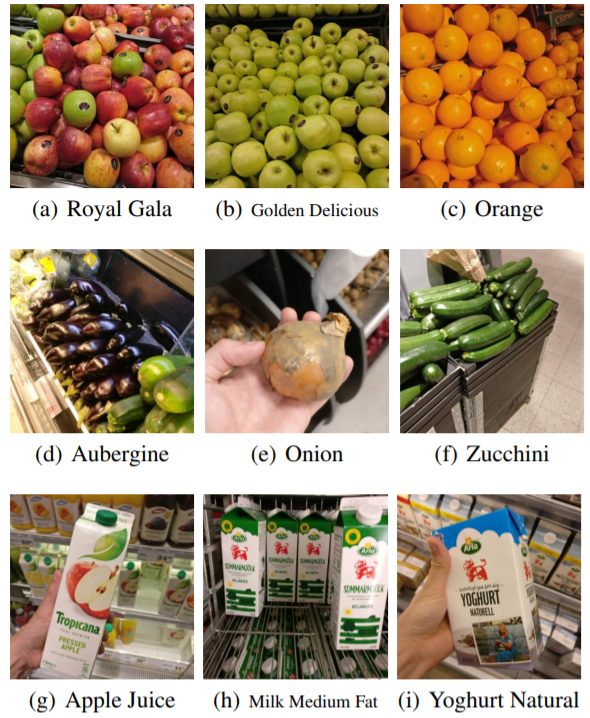
\includegraphics[scale=0.5]{PaperB/figures_and_tables/figure1.png}
		\caption{Examples of natural images in our dataset, where each image has been taken inside a grocery store. Image examples of fruits, vegetables, and refrigerated products are presented in each row respectively.}
		\label{fig:dataset_figures}
	\end{minipage}
	\hspace{10pt}
	%\vspace{-10mm}
	\begin{minipage}[b]{0.47\textwidth}
		\centering
	    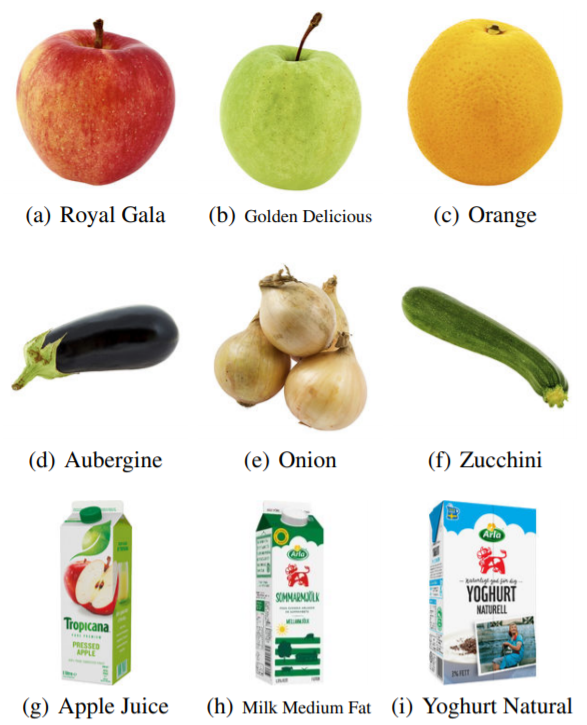
\includegraphics[scale=0.5]{PaperB/figures_and_tables/figure2.png}
		\caption{Examples of iconic images downloaded from a grocery shopping website, which corresponds to the target items in the images in Figure \ref{fig:dataset_figures}. \newline}
		\label{fig:iconic_image_figures}
	\end{minipage} 
	\vspace{-2mm}
\end{figure}



\begin{comment}

\begin{figure}
    \centering
    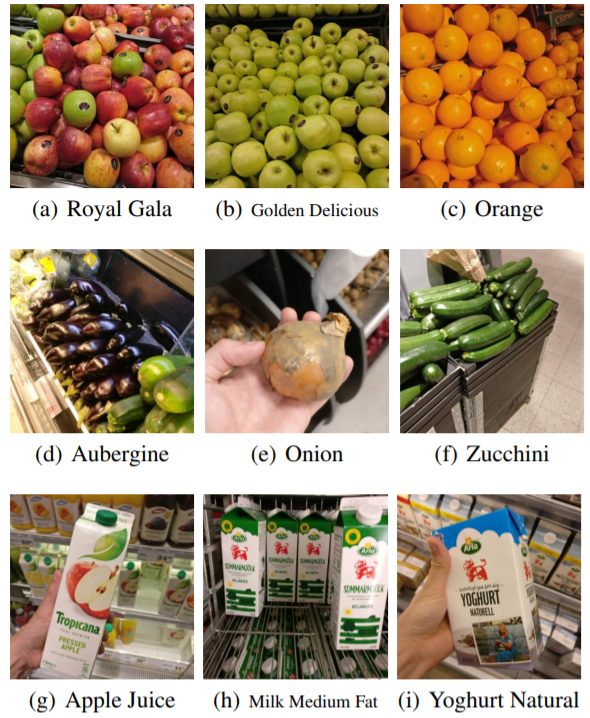
\includegraphics[scale=0.5]{PaperB/figures_and_tables/figure1.png}
    \caption{Examples of natural images in our dataset, where each image has been taken inside a grocery store. Image examples of fruits, vegetables, and refrigerated products are presented in each row respectively.}
    \label{fig:dataset_figures}
\end{figure}

\begin{figure}
    \centering
    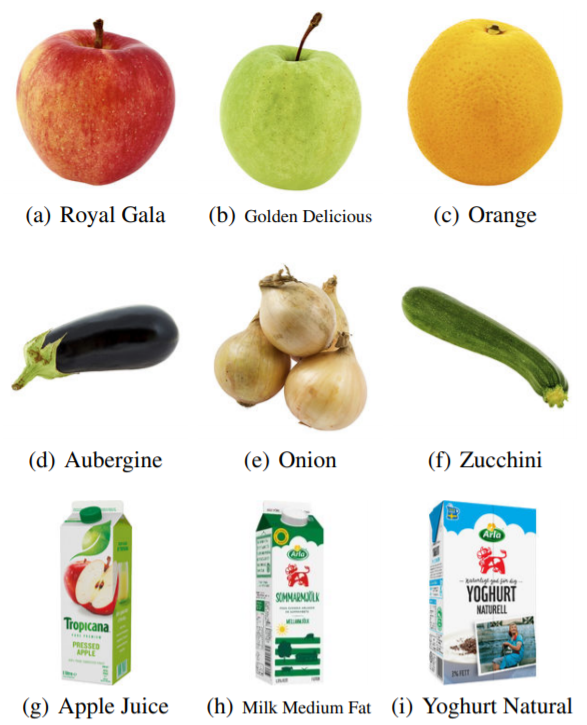
\includegraphics[scale=0.5]{PaperB/figures_and_tables/figure2.png}
    \caption{Examples of iconic images downloaded from a grocery shopping website, which corresponds to the target items in the images in Figure \ref{fig:dataset_figures}.}
    \label{fig:iconic_image_figures}
\end{figure}.
\end{comment}



For an image classification model to be capable of recognizing grocery items in the setting of grocery shopping, we need image data from grocery store environments. 
In our previous work~\citeB{B:klasson2019hierarchical}, we addressed this by collecting a novel dataset containing natural images of various raw grocery items and refrigerated products, where all images have been taken with a smartphone camera inside grocery stores to simulate a realistic shopping scenario.
In addition to the natural images, we also looked upon alternative types of grocery item data that could facilitate the classification task.
Grocery store chains commonly maintain websites where they store information about the grocery items they sell and are currently available in the store for online grocery shopping. 
For every item, there is usually an iconic image of the item with white background, a text description about the item, and also information about nutrition values, origin country, etc.
We downloaded such information from an online grocery shopping website to complement the natural images in the dataset.

To utilize the available information from the dataset for grocery item classification, we use a multi-view generative model Variational Canonical Correlation Analysis (VCCA)~\citeB{B:wang2016deep} that learns a shared representation of the natural images and the downloaded information. A view can be defined as any signal or data measured by some appropriate sensor and combining information from multiple views has previously been shown to be helpful for various image classification tasks~\citeB{B:donahue2015long-term, B:frome2013DeVISE, B:karpathy2015deep, B:kulkarni2013babytalk, B:lu2018neural, B:lu2016hierarchical, B:parikh2011relative, B:srivastava2014multimodal}. However, naively adding more additional information may not lead to improved results and even harm the performance of the model~\citeB{B:guler2014whats,B:ngiam2011multimodal}. We, therefore, perform an ablation study over the available views in the dataset with VCCA to gain insights into how each view can affect the classification performance. Moreover, VCCA allows separating the latent space into shared and private components, where the private latent spaces should hold information about a single view. This might prove useful for reducing view-specific noise in the shared latent space, which can ease the learning process of the representations we want to use for classification. We investigate the effects each view has on the learned representations of VCCA by measuring classification performances as well as visualizing the latent space for the different model settings. The contributions of this paper are the following:

\begin{itemize}[topsep=1pt, leftmargin=*] 
    \item We present a novel dataset with natural images of grocery items as well as iconic images and text descriptions for every item class (see Section 
    %subsection The Grocery Store Dataset in Results)~\citeB{B:klasson2019hierarchical}.
    \ref{paperB:sec:grocery_store_dataset})~\citeB{B:klasson2019hierarchical}.
    The natural images are taken in grocery stores in different lighting conditions and backgrounds that can be challenging settings for a computer vision-based assistive device. The additional iconic images and text descriptions make the dataset suitable for multi-view learning by combining the natural images with the extra information to obtain better classification performance.  
    
    \item We investigate how to use information from different views for the task of grocery item classification with the deep generative model VCCA (see Section \ref{paperB:sec:methods}). %subsection Methods in Experimental Procedures).
    %\ref{sec:methods}).
    This model combines information from multiple views into a low-dimensional latent representation that can be used for classification. We also select a variant of VCCA denoted VCCA-private that separates shared and private information about each view through factorization of the latent representation (see subsection Extracting Private Information of Views with VCCA-private in Experimental Procedures). 
    %\ref{sec:extracting_private_information}). 
    Furthermore, we use a standard multi-view autoencoder model called Split Autoencoder (SplitAE)~\citeB{B:ngiam2011multimodal, B:wang2015deep} for benchmarking against VCCA and VCCA-private on classification.
    
    \item We conduct experiments with SplitAE, VCCA, and VCCA-private on the task of grocery item classification with our dataset (Results).
    %Section \ref{sec:results}).
    We perform a thorough ablation study over all views in the dataset to demonstrate how each view contributes to enhancing the classification performance and conclude that utilizing the web-scraped views yields better classification results than only using the natural images (see subsection Classification Results in Results).
    % Section \ref{sec:classification_results}). 
    To gain further insights into the results, we visualize the learned latent representations of the VCCA models and discuss how the iconic images and textual descriptions impose different structures on the latent space that are beneficial for classification (see subsection Investigation of the Learned Representations in Results).
    %Section \ref{sec:investigation_of_the_learned_representations}). 
    
\end{itemize}
This work is an extended version of Klasson \etal~\citeB{B:klasson2019hierarchical}, where we first presented this dataset. In this paper, we have added a validation set of natural images from two stores that were not present in the training and test set splits from \citeB{B:klasson2019hierarchical} to avoid overfitting effects. We also demonstrate how the text descriptions can be utilized alone and along with the iconic images in a multi-view setting, while \citeB{B:klasson2019hierarchical} only experimented with the combination of natural and iconic images to build better representations of grocery items. Finally, we decode iconic images from unseen natural images as an alternative to evaluate the usefulness of the latent representations (see subsection Decoding Iconic Images from Unseen Natural Images in Results).
%(see Section \ref{sec:decoding_iconic_images}). 
As we only evaluated the decoded iconic images qualitatively in Klasson \etal~\citeB{B:klasson2019hierarchical}, we have extended the assessment by comparing the quality of the decoded images from different VCCA models with multiple image similarity metrics. 

%% RELATED WORK
Next, we discuss image datasets, food datasets, and multi-view models related to our work:

\vspace{-3mm}
\paragraph{Image Datasets} Many image datasets used in computer vision have been collected by downloading images from the web \citeB{B:deng2009imagenet, B:everingham2010pascal, B:gebru2017finegrained, B:griffin2007caltech256, B:krishna2016visualgenome, B:Krizhevsky2009cifar100, B:Lin2014MicrosoftCoco, B:nilsback2008flowers, B:song2016deep, B:WahCUB_200_2011, B:xiao2010sundatabase, B:young2014flickr30k}. 
Some datasets~\citeB{B:deng2009imagenet, B:griffin2007caltech256, B:Krizhevsky2009cifar100, B:nilsback2008flowers, B:WahCUB_200_2011} use search words with the object category in isolation, which typically returns high-quality images where the searched object is large and centered. To collect images from more real-world scenarios, searching for combinations of object categories usually returns images of two searched categories but also numerous other categories~\citeB{B:Lin2014MicrosoftCoco, B:young2014flickr30k}. 
The simplest annotation of these images is to provide a class label for the present objects. Occasionally, the dataset can use a hierarchical labeling structure and provide a fine- and coarse-grained label to objects where it is applicable. 
The annotators can also be asked to increase the possible level of supervision for the objects by, for instance, providing bounding boxes, segmentation masks, keypoints, text captions that describe the scene, and reference images of the objects~\citeB{B:gebru2017finegrained, B:krishna2016visualgenome, B:Lin2014MicrosoftCoco, B:nilsback2008flowers, B:WahCUB_200_2011, B:young2014flickr30k}. Our dataset includes reference (iconic) images of the objects that were web-scraped from a grocery store website. We also downloaded text descriptions that describe general attributes of the grocery items, such as flavor and texture, rather than the whole visual scene. The grocery items have also been labeled hierarchically in a fine- and coarse-grained manner if there exist multiple variants of specific items. For example, fine-grained classes of apples such as \textit{Golden Delicious} or \textit{Royal Gala} belongs to the coarse-grained class \textit{apple}.

\vspace{-3mm}
\paragraph{Food Datasets} 
Recognizing grocery items in their natural environments, such as grocery stores, shelves, and kitchens, have been addressed in plenty of previous works \citeB{B:geng2018fine, B:george2014recognizing, B:hsiao2010making, B:jund2016freiburg, B:klasson2019hierarchical, B:lai2011large, B:merler2007recognizing, B:singh2014bigbird, B:waltner2015mango, B:wei2019rpc, B:winlock2010toward, B:yu2018take}. The addressed tasks range from hierarchical classification, object detection, segmentation, and 3D model generation. Most of these works collect a dataset that resembles shopping or cooking scenarios, where the datasets vary in the degree of labeling, different camera views, and the data domain difference between the training and test set. 
The training sets in GroZi-120~\citeB{B:merler2007recognizing}, Grocery Products~\citeB{B:george2014recognizing}, and CAPG-GP~\citeB{B:geng2018fine} datasets were obtained by web-scraping product images of single instances on grocery web stores, while the test sets were collected in grocery stores where there can be single and multiple instances of the same item and other different items.
The RPC~\citeB{B:wei2019rpc} and TGFS~\citeB{B:yu2018take} datasets are used for object detection and classification of grocery products, where RPC is targeted for automatic checkout systems and TGFS is for the task of recognizing items purchased from self-service vending machines.
The BigBIRD~\citeB{B:singh2014bigbird} dataset and datasets from~\citeB{B:hsiao2010making, lai2011large} contain images of grocery items from multiple camera views, segmentation masks, and depth maps for 3D reconstruction of various items. 
The Freiburg Groceries~\citeB{B:jund2016freiburg} dataset contains images taken with smartphone cameras of items inside grocery stores, while its test set consists of smartphone photos in home environments with single or multiple instances from different kinds of items. The dataset presented in~\citeB{B:waltner2015mango} also contains images taken with smartphone cameras inside grocery stores to develop a mobile application for recognizing raw food items and provide details about the item, such as nutrition values and recommendations of similar items. Other works that collected datasets of raw food items, such as fruits and vegetables, focused on the standard image classification task~\citeB{B:muresan2017fruit, B:marko2013fids30} and on detecting fruits in orchards for robotic harvesting~\citeB{B:bargoti2017deepfruitdetection, B:sa2016deepfruits}. Our dataset -- the Grocery Store dataset -- shares many similarities with the mentioned works above, for instance, that all images of groceries are taken in their natural environment, the hierarchical labeling of the classes, and the iconic product images for each item in the dataset. Additionally, we have provided a text description for each item that was web-scraped along with the iconic image. As most grocery item datasets only include packaged products, we have also collected images of different fruit and vegetable classes along with packages in our dataset. 

Other examples of food datasets are those with images of food dishes, where \citeB{B:min2019survey} provides a summary of existing benchmark food datasets. The contents of these datasets range from images of food dishes~\citeB{B:bossard2014food101, B:kawano2014automatic, B:min2019ingredient, B:rich2016towards}, cooking videos~\citeB{B:damen2018scaling}, recipes~\citeB{B:marin2019learning, B:salvador2017learning, B:yagcioglu2018recipeqa}, and also restaurant-oriented information~\citeB{B:beijbom2015menu, B:xu2015geolocalized}. One major difference between recognizing groceries and food dishes is the appearance of the object categories in the images. For instance, a fruit or vegetable is usually intact and present in the image, while ingredients that are significant for recognizing a food dish may not be visible at all depending on the recipe. However, recognizing raw food items and dishes share similarities since they can appear with many different visual features in the images compared to packaged groceries, e.g., carton boxes, cans, and bottles, where the object classes have identical shape and texture. 
Another key difference is the natural environments and scenes where the images of grocery items and food dishes have been taken. Food dish images usually show the food on a plate placed on a table and, occasionally, with cutlery and a glass next to the plate. Images taken in grocery stores can cover many instances of the same item stacked close to each other in shelves, baskets, and refrigerators, while there can be multiple different kinds of items next to each other in a kitchen environment. 
To summarize, recognizing grocery items and food dishes are both challenging tasks because examples from the same category can look very different and also appear in various realistic settings in images.

\vspace{-3mm}
\paragraph{Multi-View Learning Models} There exist lots of multi-view learning approaches for data fusion of multiple features~\citeB{B:baltruvsaitis2018multimodal, B:cremer2018importance, B:frome2013DeVISE, B:fu2016semi, B:karpathy2015deep, B:ngiam2011multimodal, B:pieropan2014audio,  B:salzmann2010factorized, B:shi2019variational, B:suzuki2016joint, B:tsai2018learning, B:vedantam2017generative, B:wang2016deep, B:wu2018multimodal, B:xian2018zero, B:xu2013survey, B:zhang2016inter, B:zhao2017multi}. A common approach is to obtain a shared latent space for all views with the assumption that each view has been generated from this shared space~\citeB{B:xu2013survey}. A popular example of this is approach is Canonical Correlation Analysis (CCA)~\citeB{B:hotelling1936relations}, which aims to project two sets of variables (views) into a lower-dimensional space so that the correlation between the projections is maximized. Similar methods propose maximizing other alignment objectives for embedding the views, such as ranking losses~\citeB{B:frome2013DeVISE, B:fu2016semi, B:karpathy2015deep, B:xian2018zero}. 
There exist nonlinear extensions of CCA, e.g., Kernel CCA~\citeB{B:akaho2006kernel} and Deep CCA~\citeB{B:andrew2013deep}, that optimize their nonlinear feature mappings based on the CCA objective. 
Deep Canonically Correlated Autoencoders (DCCAE)~\citeB{B:wang2015deep} is a Deep CCA model with an autoencoding part, which aims to maximize the canonical correlation between the extracted features as well as reconstructing the input data. 
Removing the CCA objective reduces DCCAE to a standard multi-view autoencoder, e.g., Bimodal Autoencoders and Split Autoencoders (SplitAEs)~\citeB{B:ngiam2011multimodal, B:wang2015deep}, that only aim to learn a representation that best reconstructs the input data. SplitAEs aim to reconstruct two views from a representation encoded from one of the views. This approach was empirically shown to work better than Bimodal Autoencoders in \citeB{B:ngiam2011multimodal} in situations where only a single view is present at both training and test time.

Variational CCA (VCCA)~\citeB{B:wang2016deep} can be seen as an extension of CCA to deep generative models, but can also be described as a probabilistic version of SplitAEs.
VCCA uses the amortized inference procedure from Variational Autoencoders (VAEs)~\citeB{B:kingma2013auto, B:zhang2018advances} to learn the shared latent space by maximizing a lower bound on the data log-likelihood of the views. Succeeding works have proposed new learning objectives and inference methods for enabling conditional generation of views, e.g., generating an image conditioned on some text and vice versa~\citeB{B:cremer2018importance, B:shi2019variational, B:suzuki2016joint, B:vedantam2017generative, B:wu2018multimodal}. These approaches rely on fusing the views into the shared latent space as the inference procedure, which often requires tailored training and testing paradigms when views are missing. However, adding information from multiple views may not lead to improved results and can even make the model perform worse on the targeted task~\citeB{B:guler2014whats, B:ngiam2011multimodal}. This is especially the case when views have noisy observations, which complicates learning a shared latent space that combines the commonalities between the views. To avoid disturbing the shared latent space with noise from single views, some works design models which extend the shared latent space with private latent spaces for each view that should contain the view-specific variations to make learning the shared variations easier~\citeB{B:hyvarinen2000independent, B:salzmann2010factorized, B:tsai2018learning, B:wang2016deep, B:zhang2016inter}. VCCA can be extended to extract shared and private information between different views through factorization of the latent space into shared and private parts. In this paper, we investigate if the classification performance of grocery items in natural images can be improved by extracting the view-specific variations in the additional views (iconic images and product descriptions) from the shared latent space with this variant of VCCA called VCCA-private. We will experiment with treating each data point as pairs of natural images and either iconic images or text descriptions as well as triplets of natural images, iconic images, and text descriptions.
A difference between how we apply VCCA to our dataset compared to the works above is that the iconic image and text description are the same for every natural image of a specific class.  




\section{Results}\label{paperB:sec:results}

In this section, we begin by providing the details about the collected dataset, which we have named the Grocery Store dataset. Furthermore, we illustrate the utility of the additional information in the Grocery Store dataset to classify grocery items in the experiments. We compare SplitAE, VCCA, and VCCA-private with different combinations of views against two standard image classifiers. Additionally, we experiment with a vanilla autoencoder (denoted as AE) and a VAE that post-processes the natural image features to train a linear classifier cheaper and compare the performance against the multi-view models. We measure the classification performance on the test set for every model and also compare the classification accuracies when the number of words in the text description varies for the models concerned (see subsection Classification Results in Results).
%(Section \ref{sec:classification_results}).
To gain insights on how the additional views affect the learned representations, we visualize the latent spaces of VCCA and VCCA-private with PCA and discuss how different views changes the structure of the latent space (see subsection Investigation of the Learned Representations in Results).
%(Section \ref{sec:investigation_of_the_learned_representations}).
Finally, we show how iconic images can be used for enhancing the interpretability of the classification (see subsection Decoding Iconic Images from Unseen Natural Images in Results),
%(Section \ref{sec:decoding_iconic_images}), 
which was also illustrated by Klasson \etal~\citeB{B:klasson2019hierarchical}.


\subsection{The Grocery Store Dataset}
\label{paperB:sec:grocery_store_dataset}

%%% Figure 3

\begin{figure}[t]
    \centering
    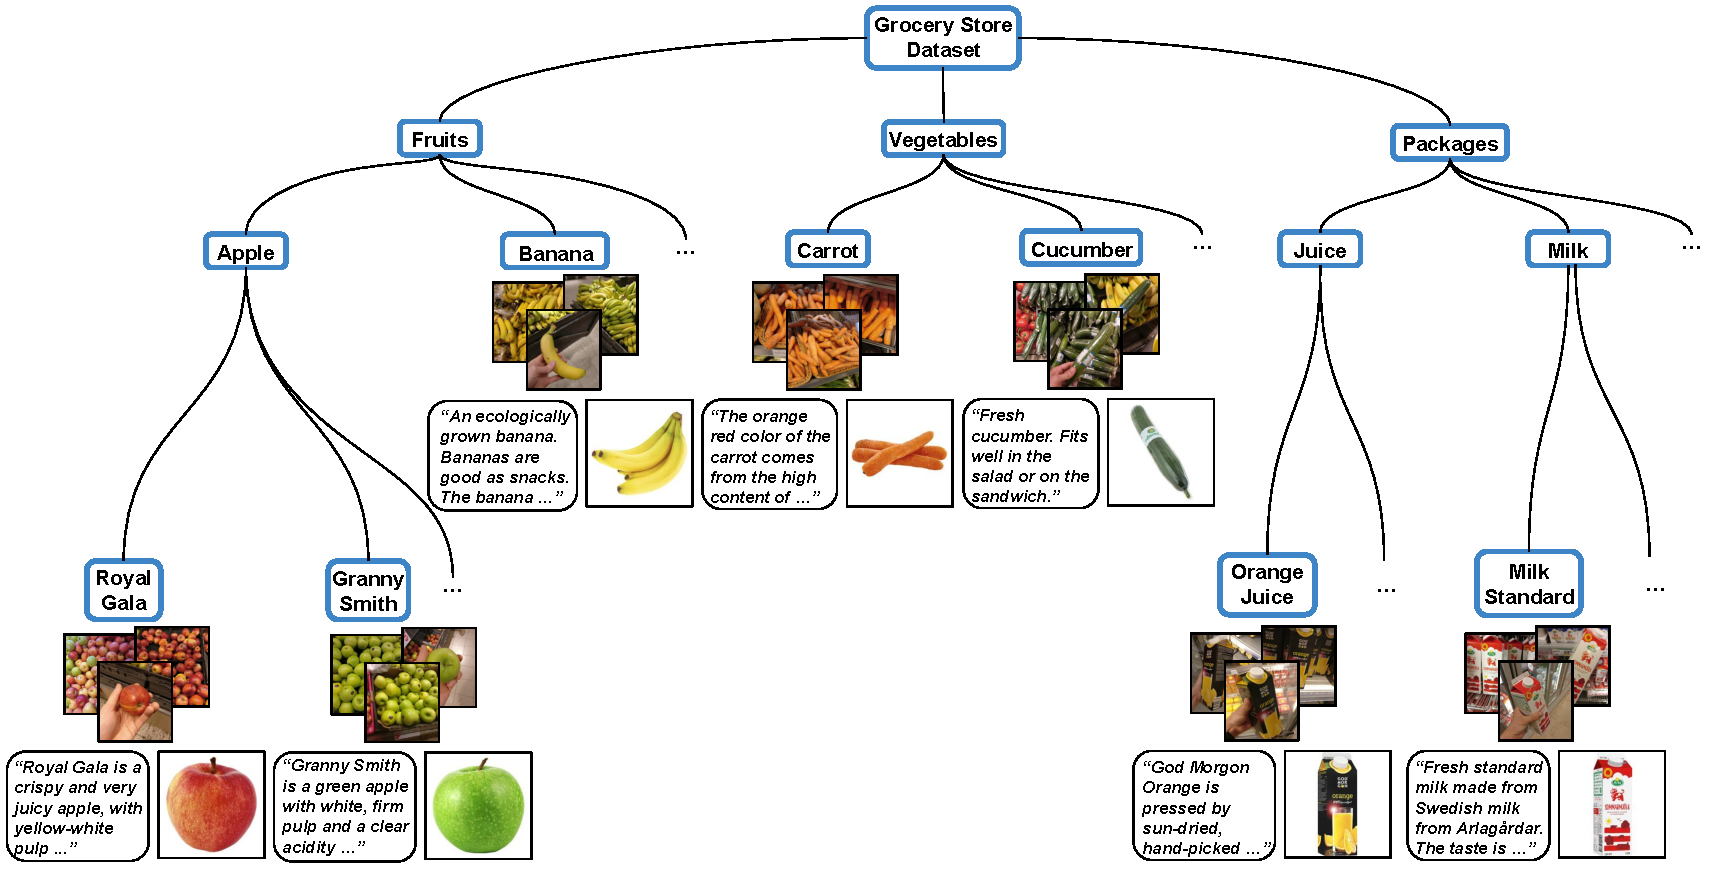
\includegraphics[width=\textwidth]{PaperB/figures_and_tables/dataset_figures/dataset_figure_new.pdf} %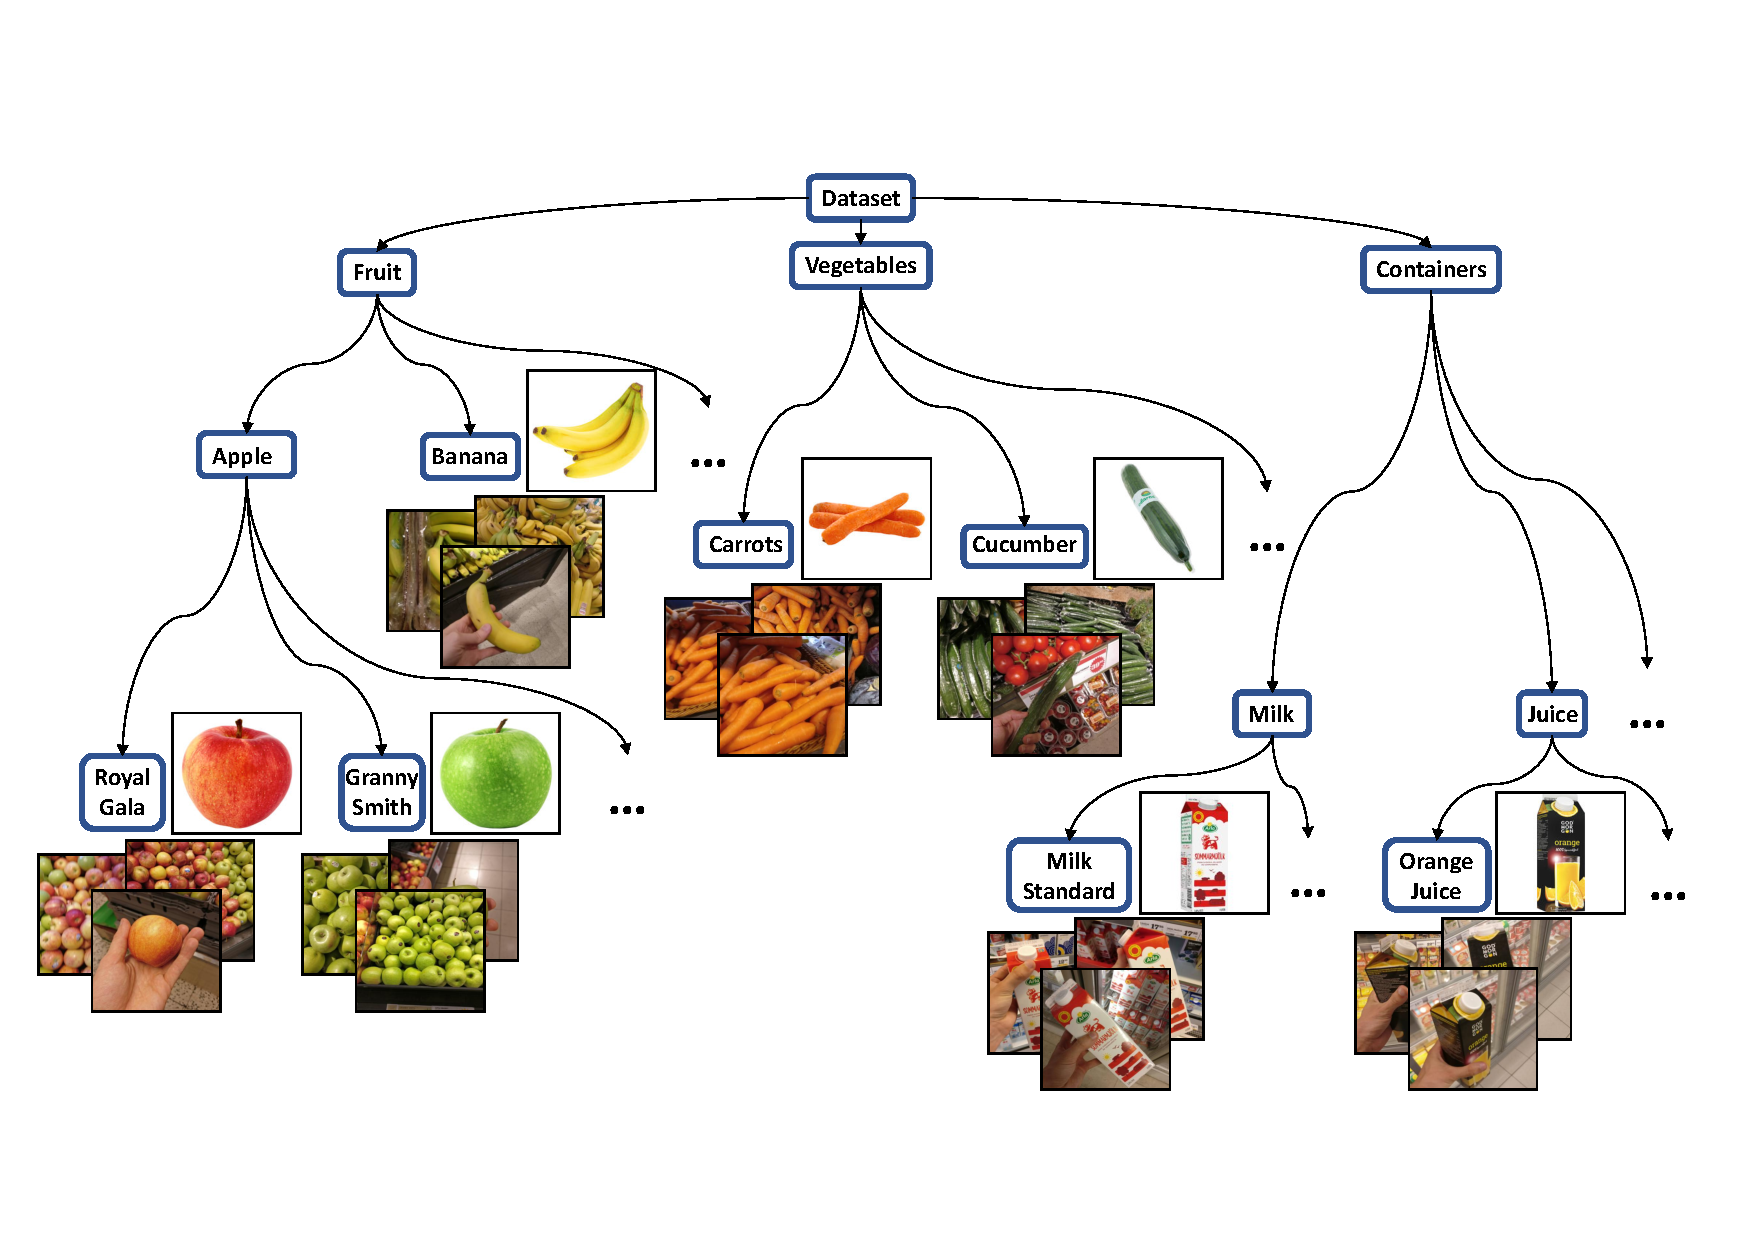
\includegraphics[width=0.95\textwidth]{dataset_figures/intro.pdf}
    \vspace{-2mm}
    \caption{Illustration of the hierarchical class structure of the dataset. First, the classes are divided by their grocery item type, i.e., \textit{Fruits}, \textit{Vegetables}, and \textit{Packages}, followed by a separating the items into coarse-grained classes, e.g., \textit{Apple}, \textit{Carrot}, and \textit{Milk}, and then into fine-grained classes. There are 81 fine-grained classes in total and 46 coarse-grained classes. The figure also shows the iconic image and text description of the items next to the class label.
   }
    \label{fig:examples} 
\end{figure}

In Klasson \etal~\citeB{B:klasson2019hierarchical}, we collected images from fruit, vegetable, and refrigerated sections with dairy and juice products in 20 different grocery stores.
The dataset consists of 5421 images from 81 different classes. For each class, we have downloaded an iconic image of the item, a text description, and information including origin country, appreciated weight and nutrient values of the item from a grocery store website. Some examples of natural images and downloaded iconic images can be seen in Figure \ref{fig:dataset_figures} and \ref{fig:iconic_image_figures} respectively. Furthermore, Table S1 displays a selection of text descriptions with their corresponding iconic image. 
The text description length varies between 6 and 91 words with an average of 36 words. 
We also structure that classes hierarchically with three levels as illustrated in Figure \ref{fig:examples_paperB}. The first level divides the items into three categories; \textit{Fruits}, \textit{Vegetables}, and \textit{Packages}. The next level consists of 46 coarse-grained classes which divides the items into groups contain groups of items types, e.g., \textit{Apple}, \textit{Carrot}, \textit{Milk}. The bottom level consists of the 81 fine-grained classes, where the items are completely separated. Note that a coarse-grained class without any fine-grained classes in the dataset, e.g., \textit{Banana} and \textit{Carrot}, is considered as a fine-grained class in the classification experiments (see subsection Classification Results in Results),
%(see Section \ref{sec:classification_results}), 
where we report both fine-grained and coarse-grained classification performance of the models.

We aimed to collect the natural images under similar conditions as if they would be taken with an assistive mobile application. 
All images have been taken with a 16-megapixel Android smartphone camera from different distances and angles. 
Occasionally, the images include other items in the background or even items that have been misplaced in incorrect shelves along with the targeted item.
The lighting conditions in the images can also vary depending on where the items are located in the store. Sometimes the images are taken while the photographer is holding the item in the hand. This is often the case for refrigerated products since these containers are usually stacked compactly in the refrigerators. For these images, we have consciously varied the position of the object, such that the item is not always centered in the image or present in its entirety. We split the natural images into a training set and test set based on the application need. Since the images have been taken in several different stores at specific days and time stamps, parts of the data will have similar lighting conditions and backgrounds for each photo occasion. To remove any such biasing correlations, all images of a certain class taken at a certain store are assigned to either the training set, validation set, or test set. In the first version of the dataset~\citeB{B:klasson2019hierarchical}, we balanced the class sizes to a large extent as possible in both the training and test set, which resulted in a training and test set containing 2640 and 2485 images respectively. In this paper, we have extended the dataset with a validation set containing 296 images taken with the same smartphone camera as before. The validation set was collected from two different grocery stores than the ones in the first version to avoid the biasing correlations described above. 
Initially, we experimented with grabbing a validation set from the current training set and noticed that the trained classifiers performed exceptionally well on the validation set. However, the classifiers generalized poorly to images from the test set that were taken in other stores and therefore decided to collect the validation set in two unseen stores to avoid the biases from the training set. We show histograms representing the class distributions for the training, validation, and test splits in Figure S1.

The scenario that we wanted to depict with the dataset was using a mobile device to classify natural images visually impaired people with grocery shopping. The additional information such as the iconic images, text descriptions, and hierarchical structure of the class labels can be used to enhance the performance of the computer vision system. Since every class label is associated with a text description, the description itself can be part of the output for visually impaired persons as they may not be able to read what is printed on a carton box or a label tag on a fruit bin in the store. 

\subsection{Models}

In this section, we briefly describe the models that we apply to grocery classification. The notation of the views that are available in the Grocery Store dataset are the following:
\begin{itemize}[topsep=1pt, noitemsep]%leftmargin=*] 
    \item $x$: Natural image encoded into image feature space with an off-the-shelf convolutional neural network.
    \item $i$: Iconic image of the object class in the natural image.
    \item $w$: Text description of the object class in the natural image.
    \item $y$: Class label of the natural image.
\end{itemize}
We mainly focus on analyzing VCCA~\citeB{B:wang2016deep} for utilizing different combinations of the views and investigate how each view contributes to the classification performance of grocery items. Our primary baseline model is the SplitAE which extracts shared representations by reconstructing all views, while VCCA aims to maximize a lower bound on the data log-likelihood for all views. We also study a variant of VCCA called VCCA-private~\citeB{B:wang2016deep}, which is used for extracting private information about each view in addition to shared information across all views by factorizing the latent space. 

We compare the multi-view models against single-view methods only using the natural images for classification. As our first single-view baseline, we customize the output layer of DenseNet169~\citeB{B:huang2017densely} to %our 
the Grocery Store dataset and train it from scratch to classify the natural images, which we refer to as DenseNet-scratch in the experiments. The second baseline called Softmax is a Softmax classifier trained on the off-the-shelf features from DenseNet169 pre-trained on the ImageNet dataset~\citeB{B:deng2009imagenet}, where we extract 1664-dimensional from the average pooling layer before the classification layer in the architecture. We also experiment with AEs and VAEs for post-processing the off-the-shelf features and use a linear classifier to evaluate the models on classification. See Section \ref{paperB:sec:methods} %subsection Methods in Experimental Procedures
%See Section \ref{sec:methods} 
for a thorough description of the single- and multi-view autoencoders used in this paper. We name the single- and multi-view autoencoders using subscripts to denote the views utilized for learning the shared latent representations. For example, VCCA$_{x i}$ utilizes natural image features $x$ and iconic images $i$, while VCCA$_{x i w y}$ uses natural image features $x$ and iconic images $i$, text descriptions $w$, and class labels $y$.


\subsection{Classification Results}
\label{paperB:sec:classification_results}

We evaluated the classification accuracy on the test set for each model. We also calculate the accuracy for the coarse-grained classes with the following method: Let the input $x^{(i)}$ have a fine-grained class $y_{fg}^{(i)}$ and a coarse-grained class $y_{cg}^{(i)}$. Each fine-grained class can be mapped to its corresponding coarse-grained class using $\parents(y_{fg}^{(i)}) = y_{cg}^{(i)}$, where $\parents(\cdot)$ stands for "parent". Then we compute the coarse-grained accuracy using  
\begin{align}\label{eq:coarse_accuracy}
    \begin{split}
        \text{coarse accuracy} & = \frac{1}{N} \sum_{i=1}^{N} \left[ \parents(\hat{y}_{fg}^{(i)}) = y_{cg}^{(i)} \right], \\ 
        \hat{y}_{fg}^{(i)} & = \argmax_{y} p(y | x^{(i)}),
    \end{split}
\end{align}
where $\left[ \parents(\hat{y}_{fg}^{(i)}) = y_{cg}^{(i)} \right] = 1$ when the condition is true and $\hat{y}_{fg}^{(i)}$ is the predicted fine-grained class from the selected classifier. The classification results for all models are shown in Table \ref{tab:classification_results_on_test_set}. We group the results in the table according to the utilized views and classifier. We see that Softmax trained on off-the-shelf features outperforms DenseNet-scratch by 4\%. This result is common when applying deep learning to small image datasets, where pre-trained deep networks are transferred to a new dataset usually performs well compared to training neural networks on the dataset from scratch. Therefore, we present results using the off-the-shelf features for all other models. 


\renewcommand{\arraystretch}{1.05}
\begin{table}[th!]
\centering
\caption{Classification accuracies on the test set for all models in percentage (\%) along for each model. The subscript letters in the model names indicate the data views used in the model. The column Accuracy corresponds to the fine-grained classification accuracy. The column Coarse Accuracy corresponds to the classifying a class within the correct parent class. Results are averaged using 10 different random seeds and we report both means and standard deviations. Abbreviations: AE, Autoencoder; VAE, Variational Autoencoder; SplitAE, Split Autoencoder; VCCA, Variational Canonical Correlation Analysis.
}
\begin{tabular}{l c c} 
    \hline 
    Model & Accuracy (\%) & Coarse Accuracy (\%) \\ 
    \hline
    DenseNet-scratch & $67.33 \pm \, 1.35$ & $75.67 \pm \, 1.15$ \\ 
    \rowcolor{gray!30}
    Softmax & $71.67 \pm 0.28$ & $83.34 \pm 0.32$ \\ 
    \hline
    AE$_{x}$+Softmax & $70.69 \pm 0.82$ & $82.42 \pm 0.58$ \\ 
    \rowcolor{gray!30}
    VAE$_{x}$+Softmax & $69.20 \pm 0.46$ & $81.24 \pm 0.63$ \\ 
    \hline
    SplitAE$_{x y}$ & $70.34 \pm 0.56$ & $82.11 \pm 0.38$ \\ 
    \rowcolor{gray!30}   
    VCCA$_{x y}$ & $70.72 \pm 0.56$ & $82.12 \pm 0.61$ \\ 
    \hline
    SplitAE$_{x i}$+Softmax & $77.68 \pm 0.69$ & $87.09 \pm 0.53$ \\ 
    \rowcolor{gray!30}  
    VCCA$_{x i}$+Softmax & $77.02 \pm 0.51$ & $86.46 \pm 0.42$ \\ 
    VCCA-private$_{x i}$+Softmax & $73.04 \pm 0.56$ & $84.16 \pm 0.51$ \\ \hline 
    \rowcolor{gray!30}
    SplitAE$_{x i y}$ & $77.43 \pm 0.80$ & $87.14 \pm 0.57$ \\ 
    VCCA$_{x i y}$ &  $77.22 \pm 0.55$ & $86.54 \pm 0.51$ \\ 
    \rowcolor{gray!30}  
    VCCA-private$_{x i y}$ & $74.04 \pm 0.83$ & $84.59 \pm 0.83$ \\
    \hline
    SplitAE$_{x w}$+Softmax & $76.27 \pm 0.66$ & $86.45 \pm 0.56$ \\
    \rowcolor{gray!30}  
    VCCA$_{x w}$+Softmax & $75.37 \pm 0.46$ & $86.00 \pm 0.32$\\
    VCCA-private$_{x w}$+Softmax & $75.11 \pm 0.81$ & $85.91 \pm 0.55$ \\ \hline
    \rowcolor{gray!30} 
    SplitAE$_{x w y}$ & $75.78 \pm 0.84$ & $86.13 \pm 0.63$ \\ 
    VCCA$_{x w y}$ & $74.72 \pm 0.85$ & $85.59 \pm 0.78$ \\ 
    \rowcolor{gray!30}  
    VCCA-private$_{x w y}$ & $74.92 \pm 0.74$ & $85.59 \pm 0.67$ \\
    \hline
    SplitAE$_{x i w}$+Softmax & $77.79 \pm 0.48$ & $87.12 \pm 0.62$ \\
    \rowcolor{gray!30}  
    VCCA$_{x i w}$+Softmax & $77.51 \pm \, 0.51$ & $86.69 \pm 0.41$ \\   
    \hline
    SplitAE$_{x i w y}$  & $78.18 \pm 0.53$ & $87.26 \pm 0.46$ \\ 
    \rowcolor{gray!30}
    VCCA$_{x i w y}$ &  $77.78 \pm 0.45$ & $86.88 \pm 0.47$ \\
    \hline 
\end{tabular}
\label{tab:classification_results_on_test_set}
\end{table}

The SplitAE and VCCA models surpass the Softmax baseline in classification performance when incorporating either the iconic image or text description view. 
We believe that the models using the iconic images achieve better classification accuracy over models using the text description because the iconic images contain visual features, e.g., color and shape of items, that are more useful for the image classification task. The text descriptions include more often information about the flavor, origin, and cooking details rather than describing visual features of the item, which can be less informative when classifying items from images. In most cases, the corresponding SplitAE and VCCA models perform on par for classification performance. However, VCCA-private with iconic images results in a significant drop in accuracy compared to its counterpart. We observed that the private latent variable simply models noise since there is only a single iconic image (and text description) for each class. We provide a further explanation of this phenomenon in Section \ref{paperB:sec:investigation_of_the_learned_representations}. 
%subsection Investigation of the Learned Representations in Results.
%Section \ref{sec:investigation_of_the_learned_representations}. 

%%% Figure 4

\begin{figure}[t]
     \centering
     \begin{subfigure}[b]{0.45\textwidth}
         \centering
         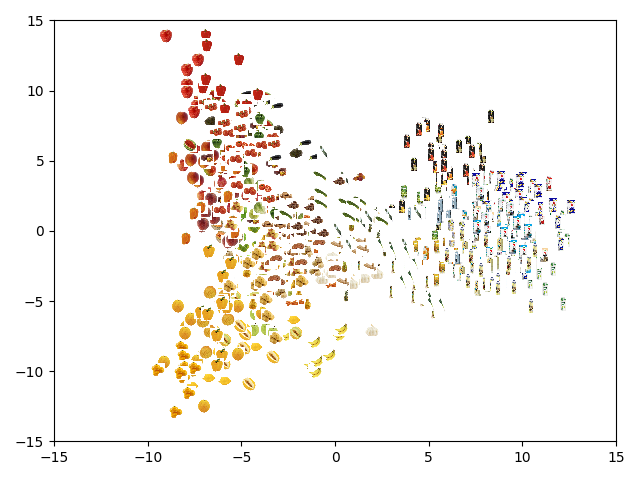
\includegraphics[width=\textwidth]{PaperB/figures_and_tables/latent_space_visualizations/splitae_vcca_comparison/pca_latents_splitae_xiwy_seed2.png}
         \caption{SplitAE$_{xiwy}$}
         \label{fig:splitae_xiwy_comparison}
     \end{subfigure}
     %\hfill
     \begin{subfigure}[b]{0.45\textwidth}
         \centering
         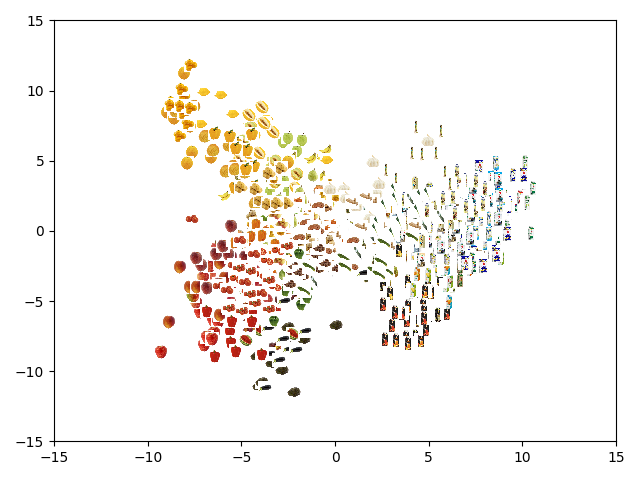
\includegraphics[width=\textwidth]{PaperB/figures_and_tables/latent_space_visualizations/splitae_vcca_comparison/pca_latents_vcca_xiwy_seed2.png}
         \caption{VCCA$_{xiwy}$}
         \label{fig:vcca_xiwy_comparison}
     \end{subfigure} \\
     %\hfill
     \begin{subfigure}[b]{0.45\textwidth}
         \centering
         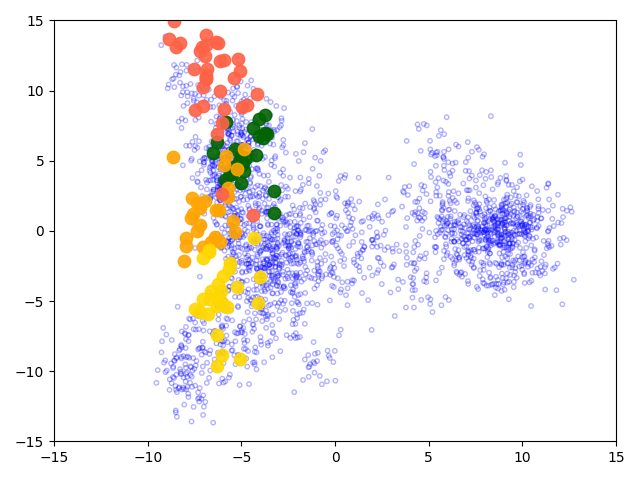
\includegraphics[width=\textwidth]{PaperB/figures_and_tables/latent_space_visualizations/splitae_vcca_comparison/pca_latent_peppers_splitae_xiwy_seed2.png}
         \caption{SplitAE$_{xiwy}$}
         \label{fig:splitae_xiwy_bell_peppers_comparison}
     \end{subfigure}
     \begin{subfigure}[b]{0.45\textwidth}
         \centering
         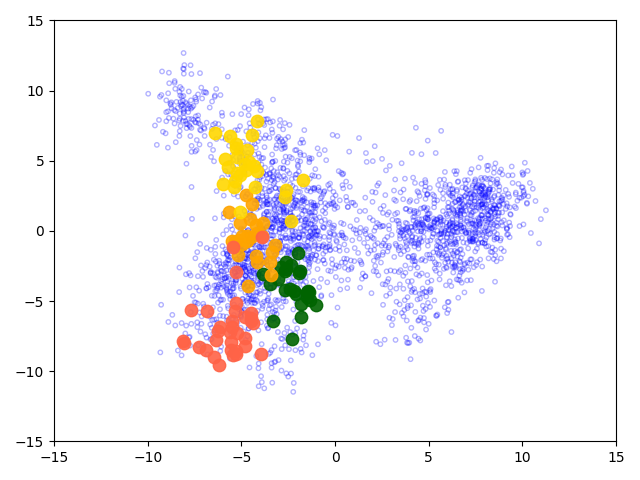
\includegraphics[width=\textwidth]{PaperB/figures_and_tables/latent_space_visualizations/splitae_vcca_comparison/pca_latent_peppers_vcca_xiwy_seed2.png}
         \caption{VCCA$_{xiwy}$}
         \label{fig:vcca_xiwy_bell_peppers_comparison}
     \end{subfigure}
        \caption{Visualizations of the latent representations of the test set from SplitAE$_{xiwy}$ and VCCA$_{xiwy}$. We plot the corresponding iconic image to each latent representation in Figure \ref{fig:splitae_xiwy_comparison} and \ref{fig:vcca_xiwy_comparison}. In Figure \ref{fig:splitae_xiwy_bell_peppers_comparison} and \ref{fig:vcca_xiwy_bell_peppers_comparison}, we plot the bell pepper representations according to the color of the class, while the blue points correspond to the other grocery items. Abbreviations: SplitAE, Split Autoencoder; VCCA, Variational Canonical Correlation Analysis.}
        \label{fig:2d_visualizations_pca_splitae_vcca_comparison}
\end{figure}

We observe that VCCA models compete with their corresponding SplitAE models in the classification task. The main difference between these models is the Kullback-Leibler (KL) divergence~\citeB{B:kullback1951information} term in the ELBO that encourages a smooth latent space for VCCA (see Section \ref{paperB:sec:experimental_procedures}). %Experimental Procedures). 
In contrast, SplitAE learns a latent space that best reconstructs the input data, which can result in parts of the space that does not represent the observed data. We showcase these differences by plotting the latent representations of SplitAE$_{x i w y}$ and VCCA$_{x i w y}$ using PCA in Figure \ref{fig:2d_visualizations_pca_splitae_vcca_comparison}. In Figure \ref{fig:splitae_xiwy_comparison} and \ref{fig:vcca_xiwy_comparison}, we have plotted the corresponding iconic image for the latent representations. We observe that VCCA$_{x i w y}$ tries to establish a smooth latent space by pushing visually similar items closer to each other, but at the same time prevent spreading out the representations too far from the origin. Figure \ref{fig:splitae_xiwy_bell_peppers_comparison} and \ref{fig:vcca_xiwy_bell_peppers_comparison} shows the positions of the bell peppers items in the latent spaces, where the color of the point corresponds to the specific bell pepper class. In Figure \ref{fig:splitae_xiwy_bell_peppers_comparison}, we observe that SplitAE$_{x i w y}$ has spread out the bell peppers across the space, while VCCA$_{x i w y}$ establishes shorter distances between them in Figure \ref{fig:vcca_xiwy_bell_peppers_comparison} due to the regularization.


%%% Figure 5

\begin{figure}[t]
    \centering
    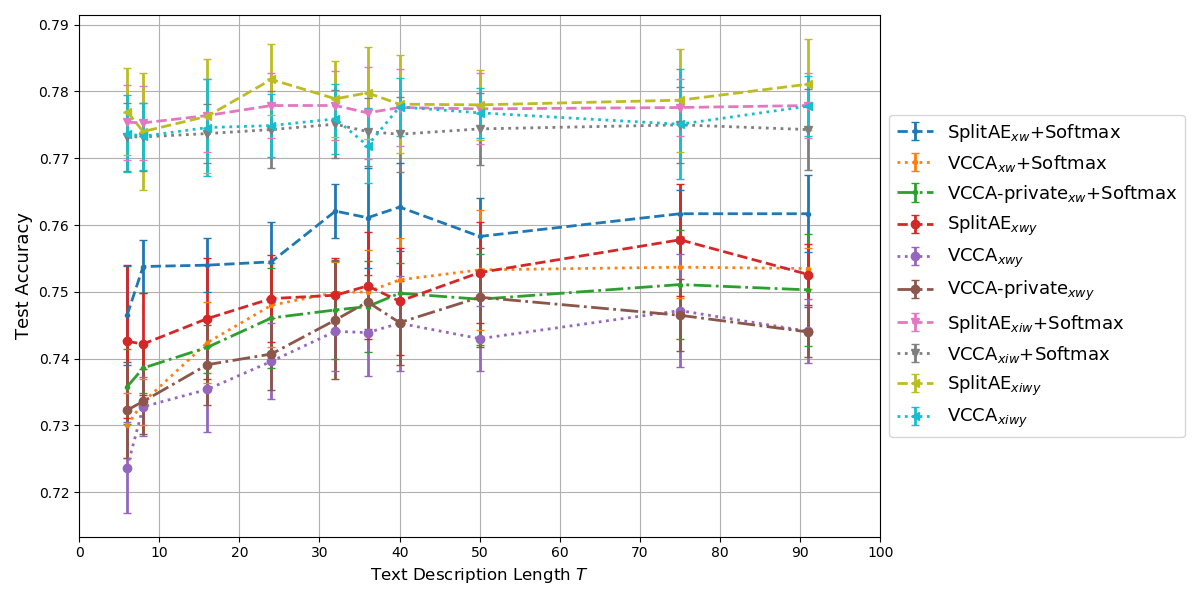
\includegraphics[width=0.95\textwidth]{PaperB/figures_and_tables/varying_t_NEW2.png}
    \caption{Test accuracy over the text description length $T$ for all SplitAE, VCCA, and VCCA-private models using the text description. We show the accuracy for the models trained with $T = 6, 8, 16, 24, 32, 36, 40, 50, 75$, and $91$ words. The results have been averaged for 10 different seeds and the error bars show the standard deviations for every setting of $T$. Abbreviations: SplitAE, Split Autoencoder; VCCA, Variational Canonical Correlation Analysis.}
    \label{fig:varying_t}
\end{figure}


We evaluated the classification performance achieved by each SplitAE, VCCA, and VCCA-private model using the text descriptions with different description lengths $T$. Figure \ref{fig:varying_t} shows the fine-grained classification accuracies for the concerned models. For models using only the text descriptions, the classification accuracies increase as $T$ increases in most cases. Setting $T \geq 32$ results in good classification performance, potentially since the models have learned to separate the grocery items based on that the text descriptions have become more dissimilar and unique. The classification accuracies are mostly stable as $T$ varies for the models with the additional iconic images. Since including iconic images significantly increases the classification performance over models only using text descriptions, we conclude that the iconic images are more helpful when we want to classify the grocery items from natural images. 





\begin{figure}[t]
     \centering
     \begin{subfigure}[b]{0.3\textwidth}
         \centering
         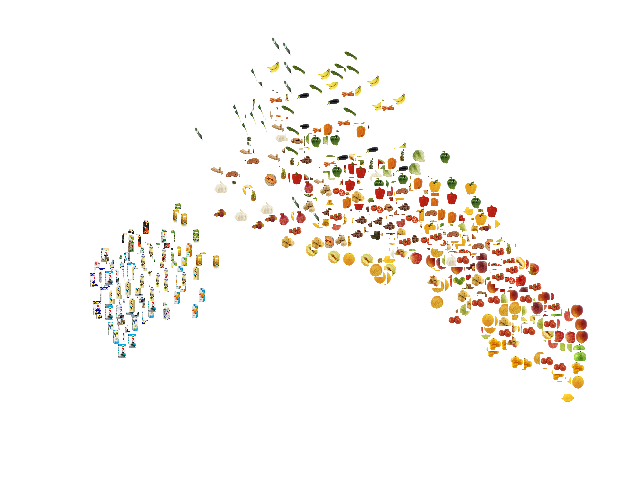
\includegraphics[width=\textwidth]{PaperB/figures_and_tables/latent_space_visualizations/pca_densenet.png}
         \caption{DenseNet169}
         \label{fig:pca_densenet}
     \end{subfigure}
     \begin{subfigure}[b]{0.3\textwidth}
         \centering
         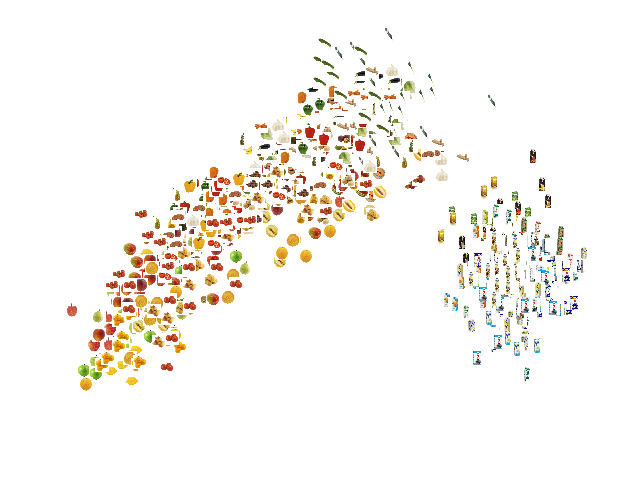
\includegraphics[width=\textwidth]{PaperB/figures_and_tables/latent_space_visualizations/pca_latents_vae_seed2.png}
         \caption{VAE$_{x}$}
         \label{fig:pca_vae_x}
     \end{subfigure} 
     \begin{subfigure}[b]{0.3\textwidth}
         \centering
         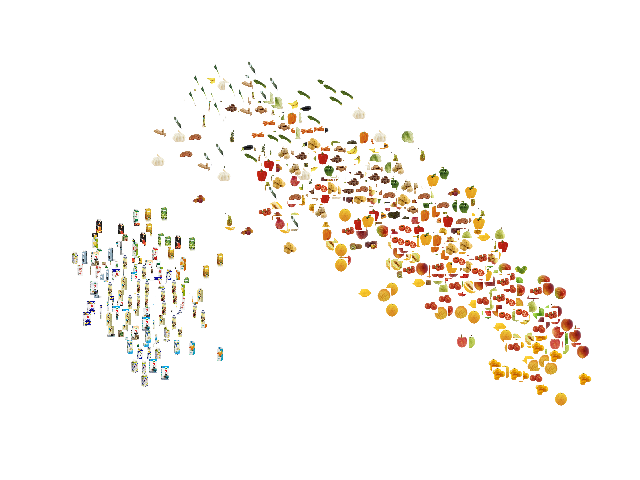
\includegraphics[width=\textwidth]{PaperB/figures_and_tables/latent_space_visualizations/pca_latents_vcca_xy_seed2.png}
         \caption{VCCA$_{x y}$}
         \label{fig:pca_vcca_xy}
     \end{subfigure} \\
     \begin{subfigure}[b]{0.3\textwidth}
         \centering
         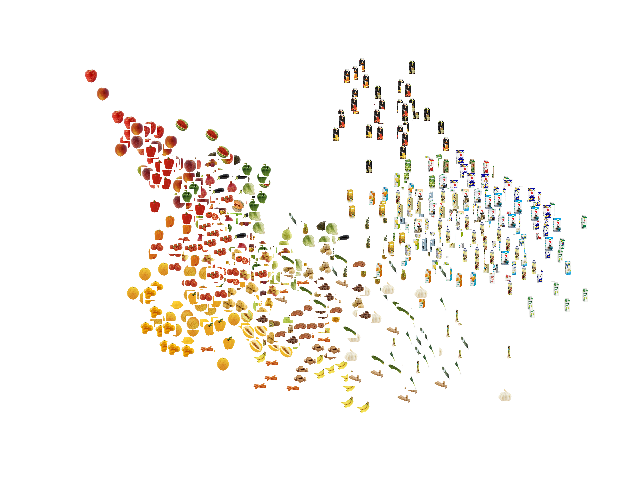
\includegraphics[width=\textwidth]{PaperB/figures_and_tables/latent_space_visualizations/pca_latents_vcca_xi_seed2.png}
         \caption{VCCA$_{x i}$}
         \label{fig:pca_vcca_xi}
     \end{subfigure} 
     \begin{subfigure}[b]{0.3\textwidth}
         \centering
         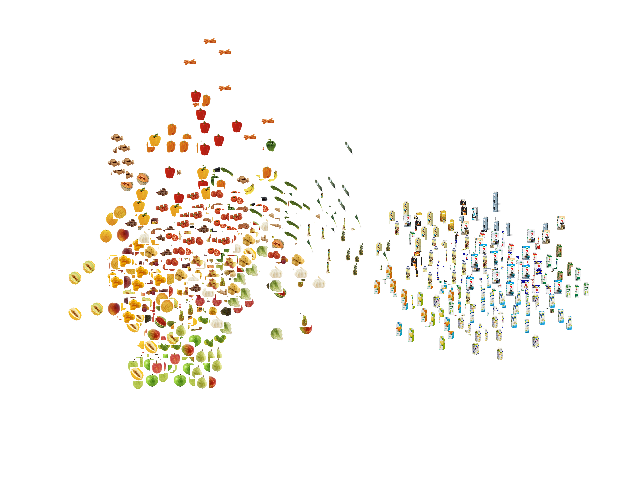
\includegraphics[width=\textwidth]{PaperB/figures_and_tables/latent_space_visualizations/pca_latents_vcca_xw_seed2.png}
         \caption{VCCA$_{x w}$}
         \label{fig:pca_vcca_xw}
     \end{subfigure} 
     \begin{subfigure}[b]{0.3\textwidth}
         \centering
         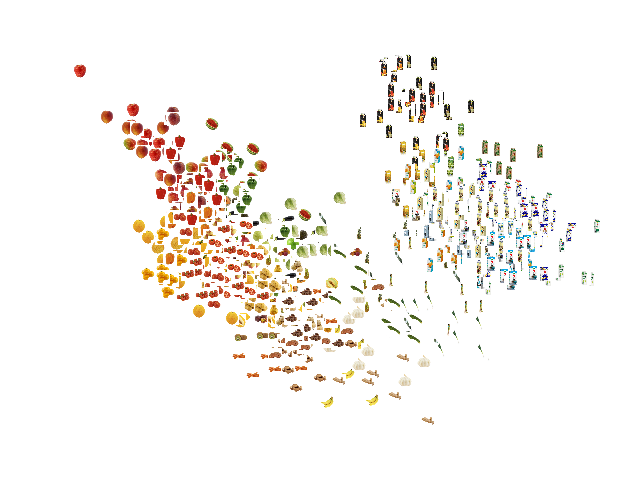
\includegraphics[width=\textwidth]{PaperB/figures_and_tables/latent_space_visualizations/pca_latents_vcca_xiw_seed2.png}
         \caption{VCCA$_{x i w}$}
         \label{fig:pca_vcca_xiw}
     \end{subfigure} \\
     \begin{subfigure}[b]{0.3\textwidth}
         \centering
         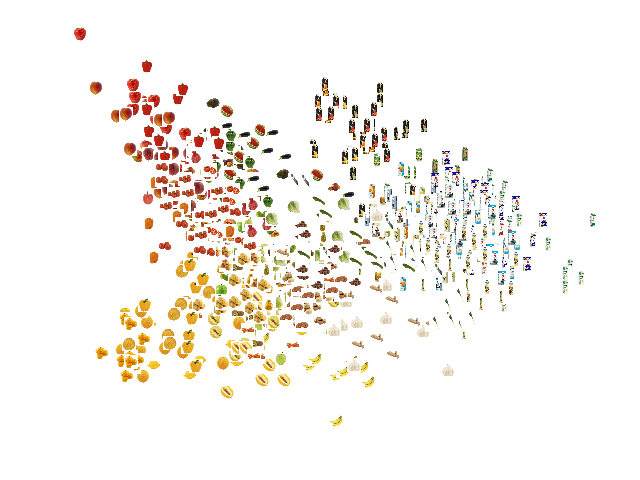
\includegraphics[width=\textwidth]{PaperB/figures_and_tables/latent_space_visualizations/pca_latents_vcca_xiy_seed2.png}
         \caption{VCCA$_{x i y}$}
         \label{fig:pca_vcca_xiy}
     \end{subfigure} 
     \begin{subfigure}[b]{0.3\textwidth}
         \centering
         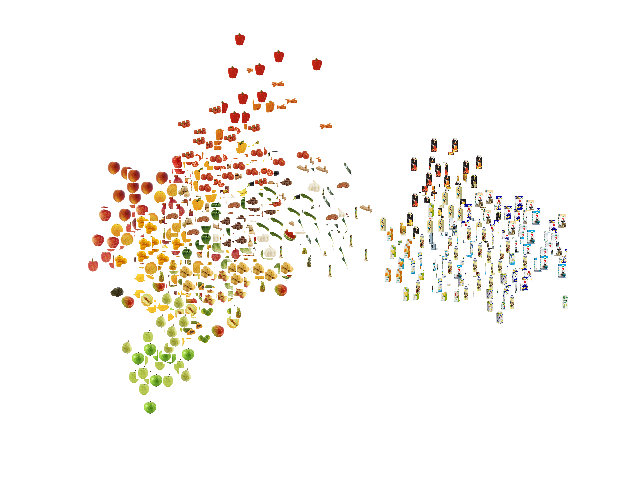
\includegraphics[width=\textwidth]{PaperB/figures_and_tables/latent_space_visualizations/pca_latents_vcca_xwy_seed2.png}
         \caption{VCCA$_{x w y}$}
         \label{fig:pca_vcca_xwy}
     \end{subfigure} 
     \begin{subfigure}[b]{0.3\textwidth}
         \centering
         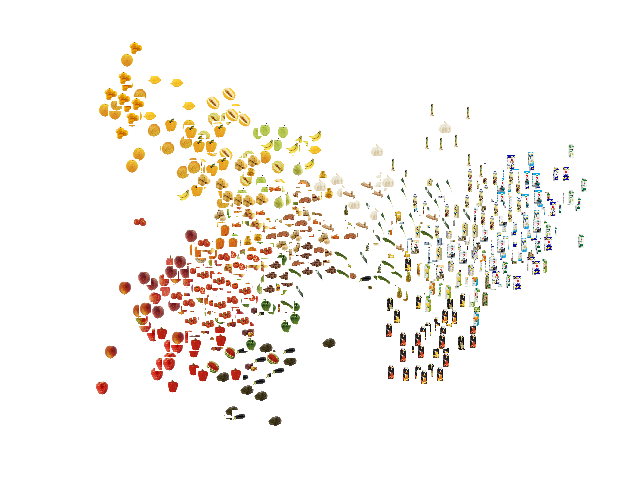
\includegraphics[width=\textwidth]{PaperB/figures_and_tables/latent_space_visualizations/pca_latents_vcca_xiwy_seed2.png}
         \caption{VCCA$_{x i w y}$}
         \label{fig:pca_vcca_xiwy}
     \end{subfigure} 
    \vspace{-2mm}
    \caption{Visualizations of the latent representations from the test set, where we plot the iconic image of the corresponding object classes. We also plot the PCA projection of the natural image features from the off-the-shelf DenseNet169 in Figure \ref{fig:pca_densenet}. All models have been initialized with the same random seed before training. %Abbreviations: VAE, Variational Autoencoder; VCCA, Variational Canonical Correlation Analysis.
    }
    \label{fig:2d_visualizations_pca}
    \vspace{-3mm}
\end{figure}


\subsection{Investigation of the Learned Representations}
\label{paperB:sec:investigation_of_the_learned_representations}

To gain insights about the effects that each view has on the classification performance, we visualize the latent space by plotting the latent representations using PCA. Utilizing the additional views showed to have similar effects on the structure of the latent spaces from SplitAE and VCCA. 
Since our main interest lies in representation learning with variational methods, we focus on studying the latent representations of VCCA and VCCA-private. 
Firstly, we use PCA to visualize the latent representations in 2D and plot the corresponding iconic images of the representations (see Figure \ref{fig:2d_visualizations_pca}). Secondly, to illustrate the effects that the iconic images and text descriptions have on the learned latent space, we focus on two cases of grocery items where one of the views helps to separate two different types of classes and the other one does not (see Figure \ref{fig:2d_visualizations_pca_apples} and \ref{fig:2d_visualizations_pca_juice_yoghurt}). Finally, we look into the shared and private latent spaces learned by VCCA-private$_{x w}$ and observe that variations in image backgrounds and structures of text sentences have been separated from the shared representations into the private ones. 

In Figure \ref{fig:2d_visualizations_pca}, we show the latent representations for the VCCA models that were used in Table \ref{tab:classification_results_on_test_set} (see subsection Classification Results in Results).
%(see Section \ref{sec:classification_results}). 
We also plot the PCA projections of the natural image features from the off-the-shelf DenseNet169 in Figure \ref{fig:pca_densenet} as a baseline. Figure \ref{fig:pca_vae_x} and \ref{fig:pca_vcca_xy} shows the latent space learned by n VAE$_{x}$ and VCCA$_{x y}$, which are similar to the DenseNet169 feature space since these models are performing compression of the natural image features into the learned latent space. We observe that these models have divided packages and raw food items into two separate clusters. However, the fruits and vegetables are scattered across their cluster and the packages have been grouped close to each other despite having different colors, e.g., black and white, on the cartons. 

The structure of the latent spaces becomes distinctly different for the VCCA models that use either iconic images or text descriptions as an additional view and we can observe the different structures that the views bring to the learned latent space. In Figure \ref{fig:pca_vcca_xi} and \ref{fig:pca_vcca_xiy}, we see that visually similar objects, in terms of color and shape, have moved closer together by utilizing iconic images in VCCA$_{x i}$ and VCCA$_{x i y}$. When using text descriptions in VCCA$_{x w}$ and VCCA$_{x w y}$, we also observe in the fruit and vegetable cluster that the items are more grouped based on their color in Figure \ref{fig:pca_vcca_xw} and \ref{fig:pca_vcca_xwy}. 
Figure \ref{fig:pca_vcca_xiw} and \ref{fig:pca_vcca_xiwy} shows the latent spaces in VCCA$_{x i w}$ and VCCA$_{x i w y}$ respectively. These latent spaces are similar to the ones learned by VCCA$_{x i}$ and VCCA$_{x i y}$ in the sense that these latent spaces also group items based on their color and shape. We believe that this structure imposed by the iconic images could be softened by reducing the scaling weight $\lambda_{i}$, which potentially could reduce the classification accuracy as a consequence. The difference between the latent spaces is not evident comparing the models using the class label.

\vspace{-3mm}
\paragraph{Red and Green Apples} To showcase how the iconic images help to learn good representations, we consider all of the apple classes in the dataset, namely the red apples \textit{Pink Lady}, \textit{Red Delicious} and \textit{Royal Gala}, and also the green apples \textit{Golden Delicious} and \textit{Granny Smith}. In Figure \ref{fig:2d_visualizations_pca_apples}, we group the red apple classes and visualize their latent representations by red points. The green apples are grouped similarly and we visualize their latent representations with green points. Latent representations of all other grocery items are visualized as blue points. The models using iconic images as one view in Figure \ref{fig:pca_vcca_xi_apples}, \ref{fig:pca_vcca_xiy_apples}, \ref{fig:pca_vcca_xiw_apples}, and \ref{fig:pca_vcca_xiwy_apples} have managed to separate the red and green apples based on their color differences. The models using text description have instead moved the apples closer together in one part of the latent space, possibly because of their similarities mentioned in the description. 

%%% Figure 7



\begin{figure}[t]
     \centering
     \begin{subfigure}[b]{0.3\textwidth}
         \centering
         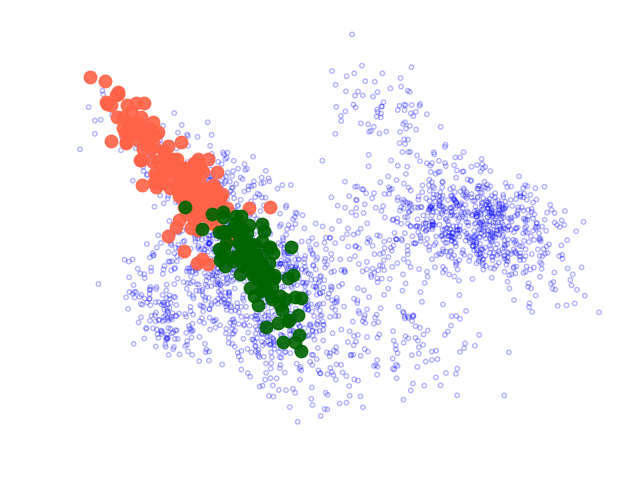
\includegraphics[width=\textwidth]{PaperB/figures_and_tables/latent_space_visualizations/apples_new/pca_latent_apples_vcca_xi_seed2.png}
         \caption{VCCA$_{x i}$}
         \label{fig:pca_vcca_xi_apples}
     \end{subfigure} 
     \begin{subfigure}[b]{0.3\textwidth}
         \centering
         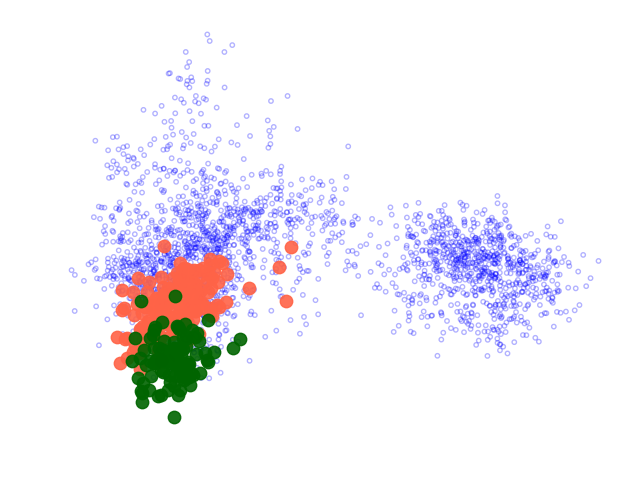
\includegraphics[width=\textwidth]{PaperB/figures_and_tables/latent_space_visualizations/apples_new/pca_latent_apples_vcca_xw_seed2.png}
         \caption{VCCA$_{x w}$}
         \label{fig:pca_vcca_xw_apples}
     \end{subfigure} 
     \begin{subfigure}[b]{0.3\textwidth}
         \centering
         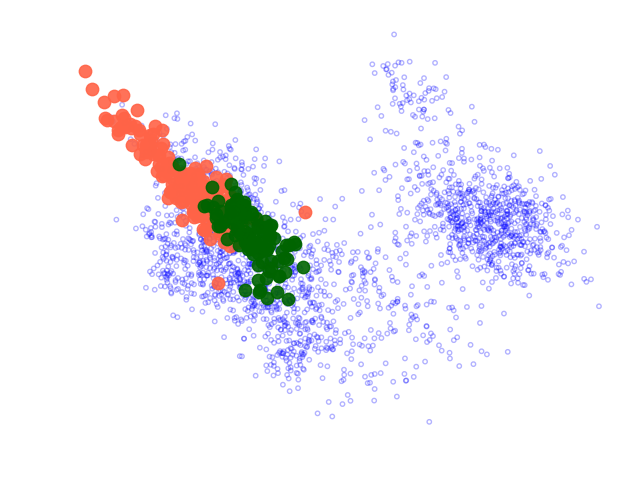
\includegraphics[width=\textwidth]{PaperB/figures_and_tables/latent_space_visualizations/apples_new/pca_latent_apples_vcca_xiw_seed2.png}
         \caption{VCCA$_{x i w}$}
         \label{fig:pca_vcca_xiw_apples}
     \end{subfigure} \\
     \begin{subfigure}[b]{0.3\textwidth}
         \centering
         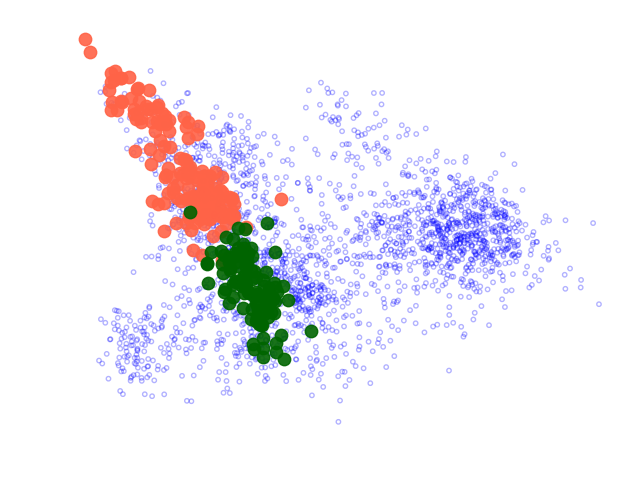
\includegraphics[width=\textwidth]{PaperB/figures_and_tables/latent_space_visualizations/apples_new/pca_latent_apples_vcca_xiy_seed2.png}
         \caption{VCCA$_{x i y}$}
         \label{fig:pca_vcca_xiy_apples}
     \end{subfigure} 
     \begin{subfigure}[b]{0.3\textwidth}
         \centering
         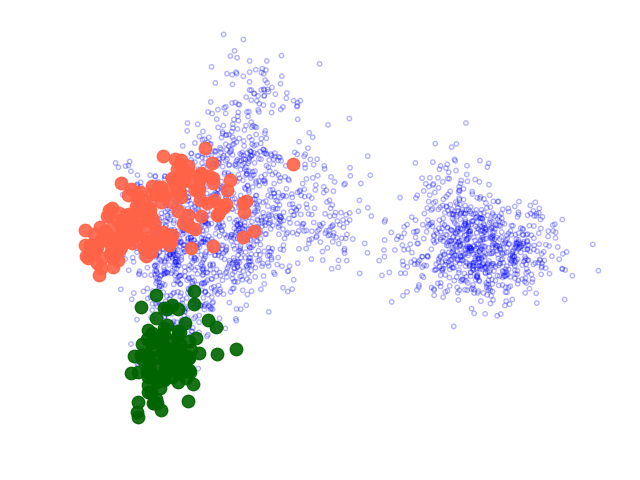
\includegraphics[width=\textwidth]{PaperB/figures_and_tables/latent_space_visualizations/apples_new/pca_latent_apples_vcca_xwy_seed2.png}
         \caption{VCCA$_{x w y}$}
         \label{fig:pca_vcca_xwy_apples}
     \end{subfigure} 
     \begin{subfigure}[b]{0.3\textwidth}
         \centering
         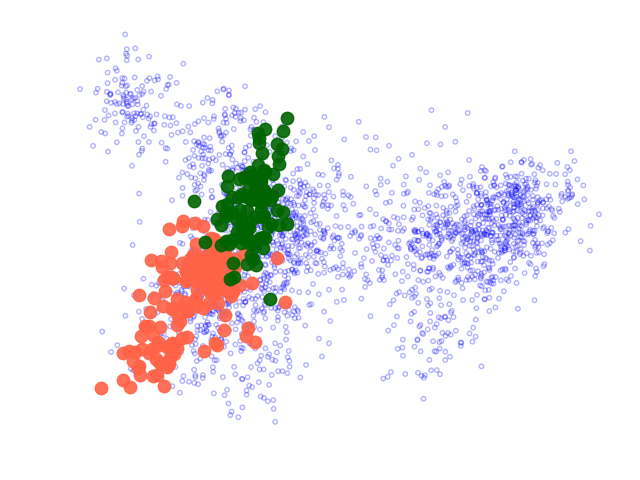
\includegraphics[width=\textwidth]{PaperB/figures_and_tables/latent_space_visualizations/apples_new/pca_latent_apples_vcca_xiwy_seed2.png}
         \caption{VCCA$_{x i w y}$}
         \label{fig:pca_vcca_xiwy_apples}
     \end{subfigure}
    \vspace{-2mm} 
    \caption{Visualizations of the latent representations $\mu_{z}$ of the red and green apples in the Grocery Store dataset. The red points correspond to the red apple classes, while the green points correspond to the green apple. The blue points correspond to the other grocery items. 
    %Abbreviations: VCCA, Variational Canonical Correlation Analysis.
    }
    \label{fig:2d_visualizations_pca_apples}
    \vspace{-3mm}
\end{figure}


\vspace{-3mm}
\paragraph{Juice and Yoghurt Packages} To illustrate how the text descriptions can establish more useful latent representations, we consider a selection of juice and yoghurt classes. These packaged items have similar shapes and colors, which makes it difficult for a classifier to distinguish their content differences using only visual input. In Figure \ref{fig:2d_visualizations_pca_juice_yoghurt}, we visualize the latent representations of the juice and yoghurt packages using yellow and green points respectively. We observe that only VCCA$_{x w}$ and VCCA$_{x w y}$ manages to separate the packages in Figure \ref{fig:pca_vcca_xw_juice_yoghurt} and \ref{fig:pca_vcca_xwy_juice_yoghurt} due to their different text descriptions. Since the iconic images of the packages are visually similar, adding this information is insufficient for separating these packages in the latent space. This indicates that we gain different benefits from the iconic images and text descriptions when it comes to classifying grocery items.

%%% Figure 8


\begin{figure}[t]
     \centering
     \begin{subfigure}[b]{0.3\textwidth}
         \centering
         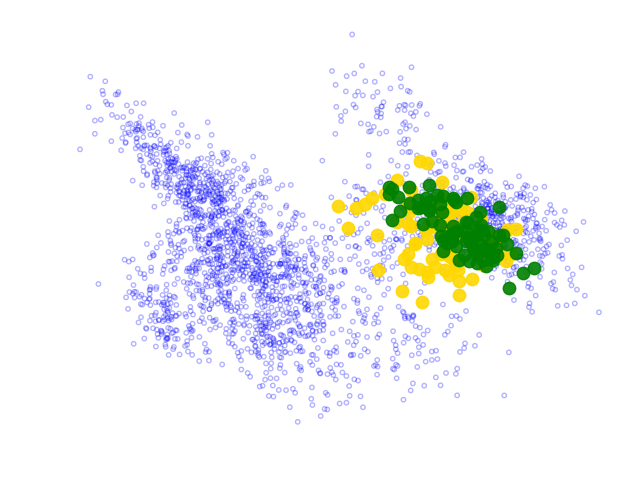
\includegraphics[width=\textwidth]{figures_and_tables/latent_space_visualizations/juice_yoghurt_new/pca_latent_juice_yoghurt_vcca_xi_seed2.png}
         \caption{VCCA$_{x i}$}
         \label{fig:pca_vcca_xi_juice_yoghurt}
     \end{subfigure} 
     \begin{subfigure}[b]{0.3\textwidth}
         \centering
         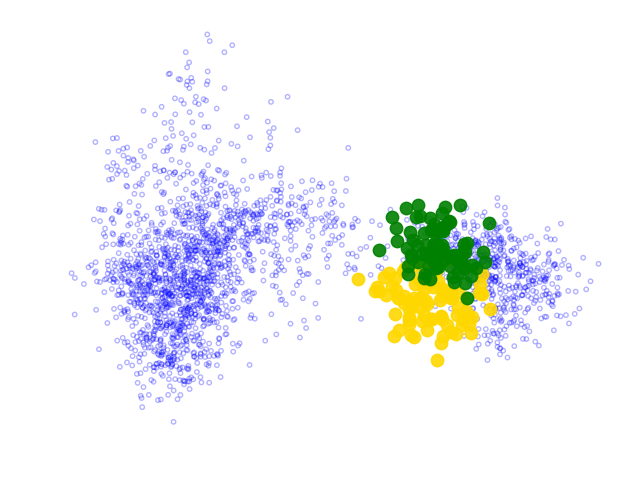
\includegraphics[width=\textwidth]{figures_and_tables/latent_space_visualizations/juice_yoghurt_new/pca_latent_juice_yoghurt_vcca_xw_seed2.png}
         \caption{VCCA$_{x w}$}
         \label{fig:pca_vcca_xw_juice_yoghurt}
     \end{subfigure} 
     \begin{subfigure}[b]{0.3\textwidth}
         \centering
         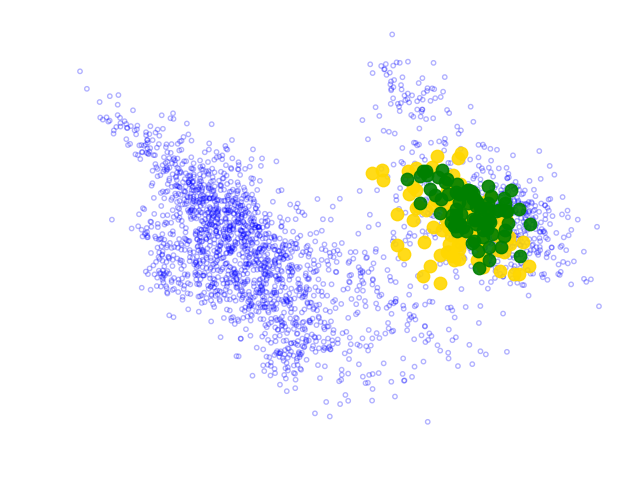
\includegraphics[width=\textwidth]{figures_and_tables/latent_space_visualizations/juice_yoghurt_new/pca_latent_juice_yoghurt_vcca_xiw_seed2.png}
         \caption{VCCA$_{x i w}$}
         \label{fig:pca_vcca_xiw_juice_yoghurt}
     \end{subfigure} \\
     \begin{subfigure}[b]{0.3\textwidth}
         \centering
         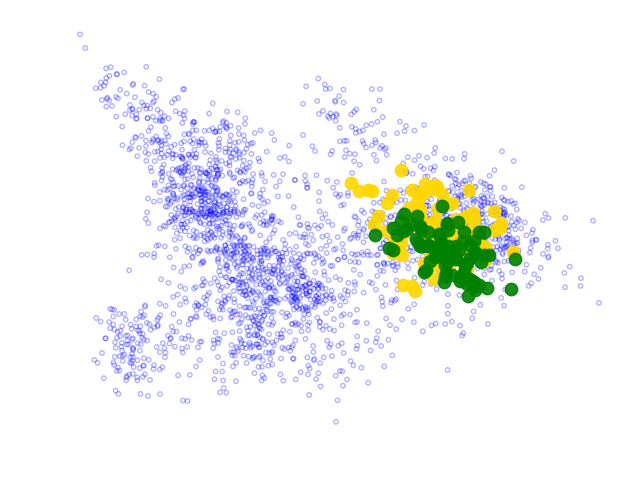
\includegraphics[width=\textwidth]{figures_and_tables/latent_space_visualizations/juice_yoghurt_new/pca_latent_juice_yoghurt_vcca_xiy_seed2.png}
         \caption{VCCA$_{x i y}$}
         \label{fig:pca_vcca_xiy_juice_yoghurt}
     \end{subfigure} 
     \begin{subfigure}[b]{0.3\textwidth}
         \centering
         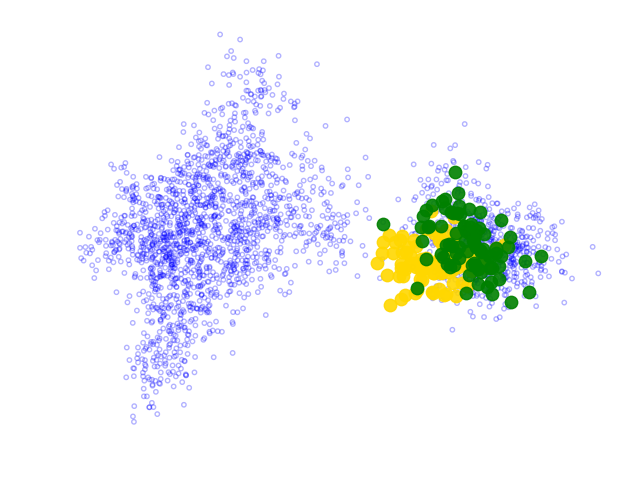
\includegraphics[width=\textwidth]{figures_and_tables/latent_space_visualizations/juice_yoghurt_new/pca_latent_juice_yoghurt_vcca_xwy_seed2.png}
         \caption{VCCA$_{x w y}$}
         \label{fig:pca_vcca_xwy_juice_yoghurt}
     \end{subfigure} 
     \begin{subfigure}[b]{0.3\textwidth}
         \centering
         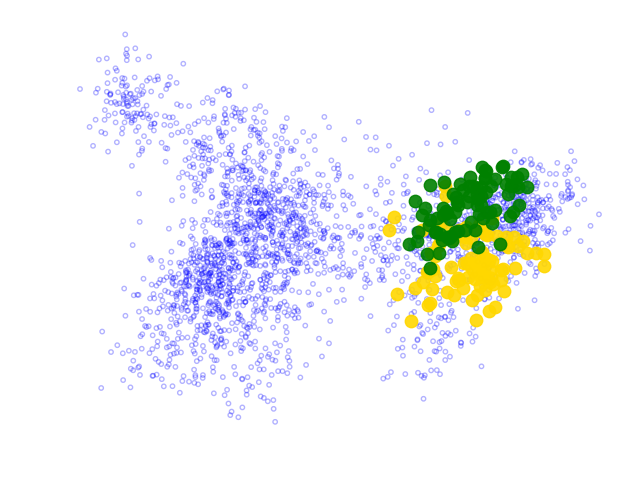
\includegraphics[width=\textwidth]{figures_and_tables/latent_space_visualizations/juice_yoghurt_new/pca_latent_juice_yoghurt_vcca_xiwy_seed2.png}
         \caption{VCCA$_{x i w y}$}
         \label{fig:pca_vcca_xiwy_juice_yoghurt}
     \end{subfigure} 
    \caption{Visualizations of the latent representations $\mu_{z}$ of a selection of juice packages and yoghurt packages in the Grocery Store dataset. The yellow and green points correspond to the juice and yoghurt packages respectively. The blue points correspond to the other grocery items. Abbreviations: VCCA, Variational Canonical Correlation Analysis.}
    \label{fig:2d_visualizations_pca_juice_yoghurt}
\end{figure}



\vspace{-3mm}
\paragraph{Latent Spaces of VCCA-private } We show the shared and private latent spaces of VCCA-private$_{x w}$ in Figure \ref{fig:2d_visualizations_pca_vcca_private_xw}b-d, as well as the single latent space of VCCA$_{x w}$ for comparison in Figure \ref{fig:pca_vcca_xw_z}. 
Comparing with the latent space of VCCA$_{x w}$, the shared latent space of VCCA-private$_{x w}$ in Figure \ref{fig:pca_vcca_private_xw_z}, has structured the raw food items based on their class, color, and shape better than standard VCCA$_{x w}$. In Figure \ref{fig:pca_vcca_private_xw_ux}, we plot the natural images corresponding to the latent representation for the private latent variable $u_{x}$. We zoom in on some natural images and found that the images are structured based on their similarities in background and camera view. On the left and bottom sides of the cluster, we found images of grocery items closely packed together in bins. Single items that are held in the hand of the photographer are placed on the right side, whereas images of items and the store floor are placed on the top and middle of the latent space. The model has therefore managed to separate the variations within the natural image view into the private latent variable $u_{x}$ from the shared latent variable $z$, which probably is the main reason why similar raw food items are closer to each other in Figure \ref{fig:pca_vcca_private_xw_z} than in Figure \ref{fig:pca_vcca_xw_z}. We also plot the corresponding iconic image on the position of the text description representation for the private latent variable $u_{w}$ in Figure \ref{fig:pca_vcca_private_xw_uw}. Note that every text description is projected at the same location in the latent space since the text descriptions are the same for every class item. We highlighted some specific words in the descriptions and observed that descriptions with the same words are usually close to each other. Visually dissimilar items can be grouped close to each other in this latent space, which indicates that the private latent variable $u_{w}$ contains information about the structure of the text sentences, i.e., word occurrences and how they are ordered in the text description. 
In Figure S4, we show the shared and private latent spaces of VCCA-private$_{x i}$ and provide a conclusion to the results in the 
Supplemental Experimental Procedures.
%supplementary material.
%In Appendix \ref{app:investigating_latent_representations_in_vcca_private_xi}, we show the shared and private latent spaces of VCCA-private$_{x i}$ in \MK{Figure S14} and provide a conclusion to the results.

%%%% Figure 9

\begin{figure}[!tp]
     \centering
     \begin{subfigure}[b]{0.49\textwidth}
         \centering
         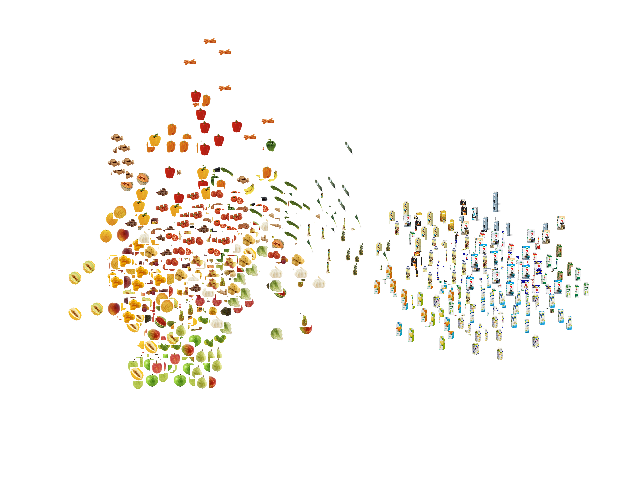
\includegraphics[width=\textwidth]{PaperB/figures_and_tables/latent_space_visualizations/pca_latents_vcca_xw_seed2.png}
         \caption{$\mu_{z}$ from VCCA$_{x w}$}
         \label{fig:pca_vcca_xw_z}
     \end{subfigure} 
     \begin{subfigure}[b]{0.49\textwidth}
         \centering
         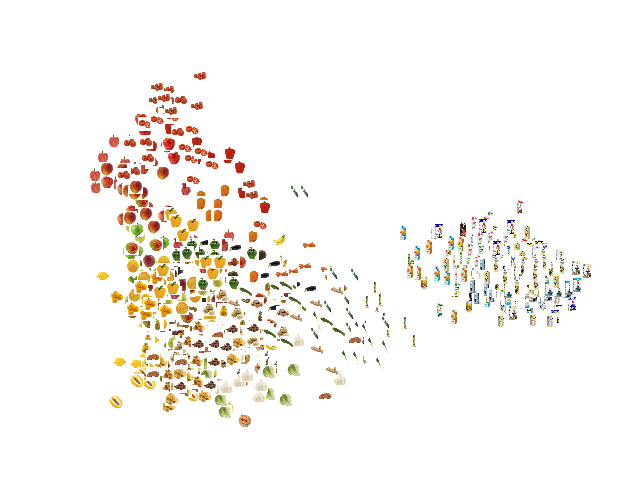
\includegraphics[width=\textwidth]{PaperB/figures_and_tables/private_latent_space_visualizations/pca_z_vaecca_private_xw_seed1.png}
         \caption{$\mu_{z}$ from VCCA-private$_{x w}$}
         \label{fig:pca_vcca_private_xw_z}
     \end{subfigure} \\
     \begin{subfigure}[b]{0.6\textwidth}
         \centering
         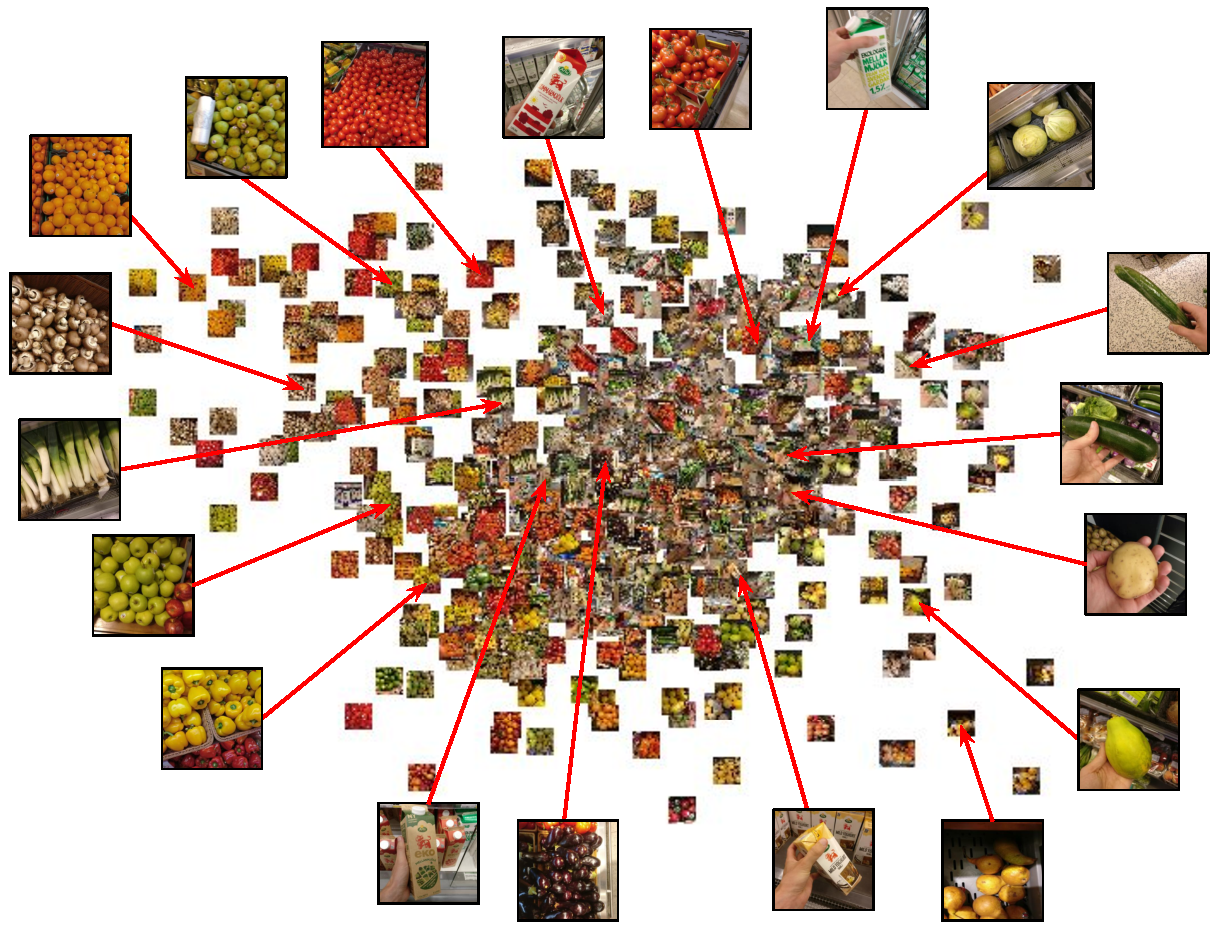
\includegraphics[width=\textwidth]{PaperB/figures_and_tables/private_latent_space_visualizations/vcca_private_ux_space.pdf}
         \caption{$\mu_{x}$ from VCCA-private$_{x w}$}
         \label{fig:pca_vcca_private_xw_ux}
     \end{subfigure} \\
     \begin{subfigure}[b]{0.7\textwidth}
         \centering
         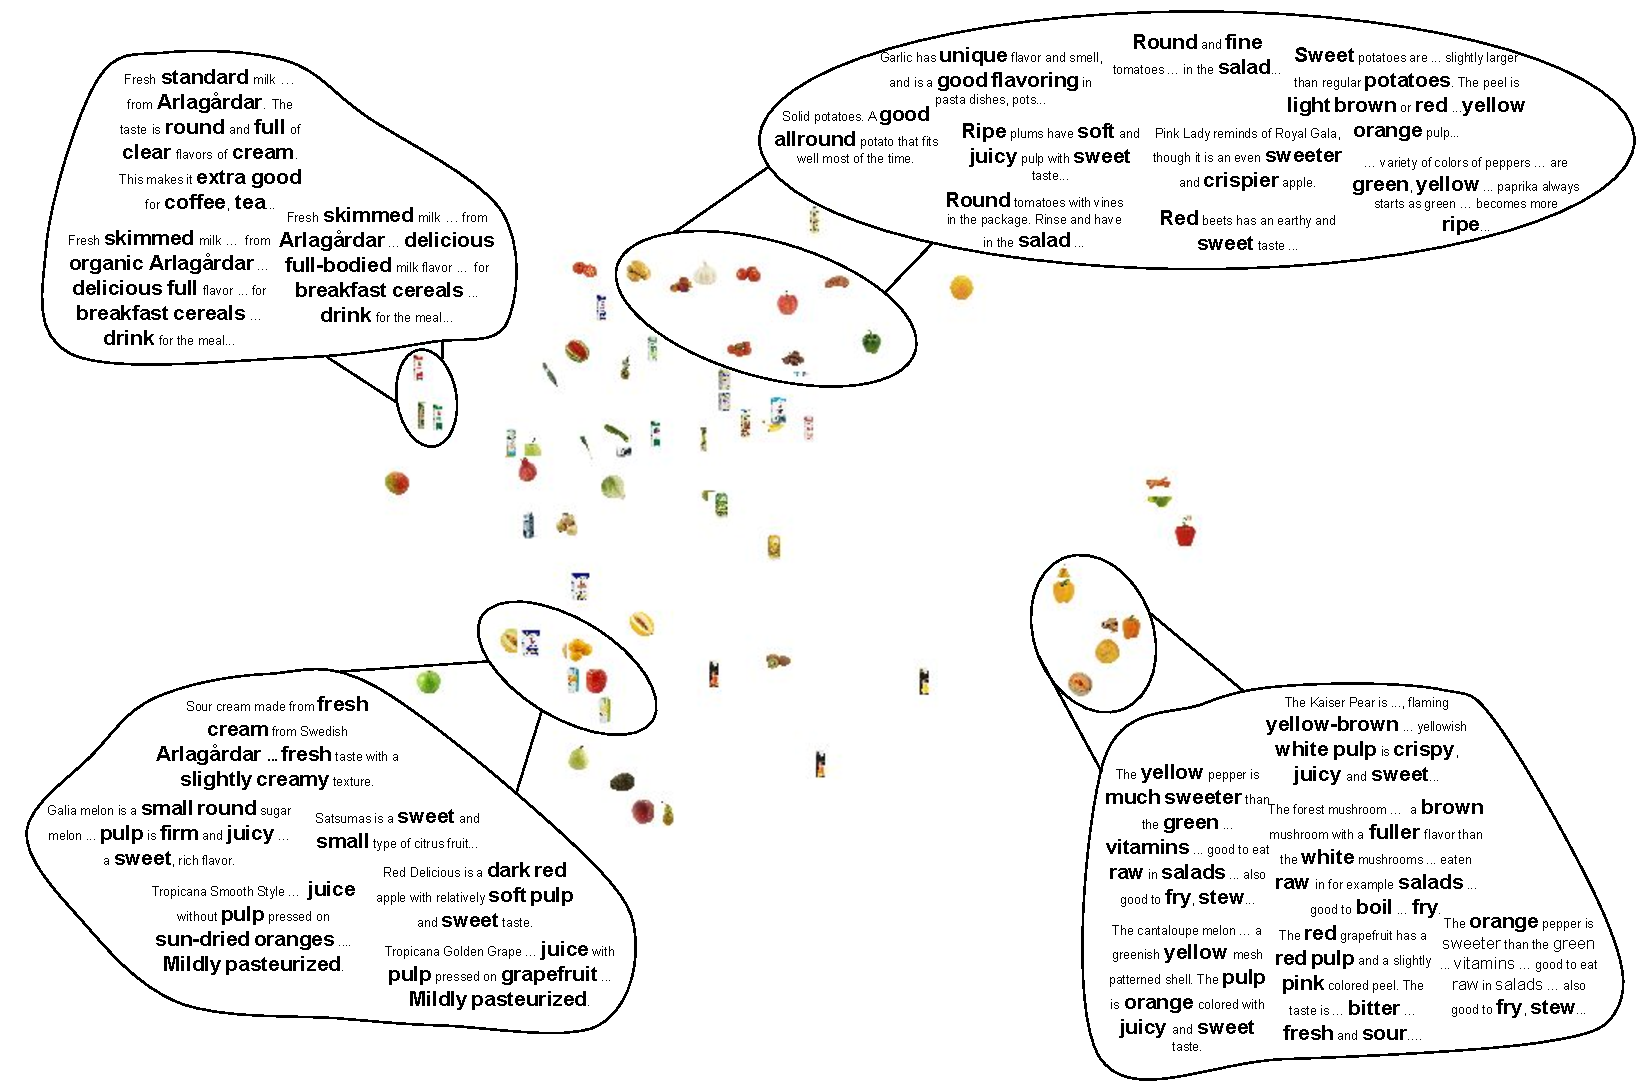
\includegraphics[width=\textwidth]{PaperB/figures_and_tables/private_latent_space_visualizations/vcca_private_uw_space.pdf}
         \caption{$\mu_{w}$ from VCCA-private$_{x w}$}
         \label{fig:pca_vcca_private_xw_uw}
     \end{subfigure} 
    \caption{Visualizations of the latent representations $\mu_{z}$ of a selection of juice packages and yoghurt packages in the Grocery Store dataset. The yellow and green points correspond to the juice and yoghurt packages respectively. The blue points correspond to the other grocery items. 
    	%Abbreviations: VCCA, Variational Canonical Correlation Analysis.
    }
    \label{fig:2d_visualizations_pca_vcca_private_xw}
\end{figure}

\subsection{Decoding Iconic Images from Unseen Natural Images}
\label{paperB:sec:decoding_iconic_images} 

In this section, we show how the iconic image decoder can decode plausible iconic images of grocery items from unseen natural images in the test set. We apply the same approach as in~\citeB{klasson2019hierarchical}, where we encode unseen natural images and then decode the retrieved latent representation back into an iconic image. We also report several image similarity metrics to investigate if the decoded image quality is correlated with classification performance.
We report peak signal-to-noise ratio (PSNR), structural similarity (SSIM)~\citeB{B:wang2004image}, and the KL divergence by comparing the decoded iconic images to the true ones. For computing the KL divergence, we model the decoded and true iconic image using two Gaussian Mixture Model (GMM)~\citeB{B:cui2015comparison, B:goldberger2003efficient}. The images are then represented as density functions, such that we can measure the similarity between the two densities with the KL divergence and use it as an image similarity metric. Since the KL divergence between two GMMs is not analytically tractable, we apply Monte Carlo simulation using $n$ i.i.d. samples drawn from the decoded image density for approximating the KL divergence~\citeB{B:hershey2007approximating}. 
Due to the simple structure of the iconic images, we fit the GMMs with $K=2$ Gaussian components using the RGB color values and draw $n=100$ Monte Carlo samples to estimate the KL divergence in all experiments. 
Table \ref{tab:iconic_image_similarity_metrics} shows the image similarity metrics between the VCCA models using the iconic images. We also show the model classification accuracy for each model, which have been taken from Table \ref{tab:classification_results_on_test_set}. 
The models perform on par on the image similarity metrics, which indicates that the quality of the decoded images is intact if the model extends to utilizing text descriptions and class labels in addition to the iconic images.

In Figure \ref{fig:decoded_iconic_images_with_metrics}, we display five different natural images from the test set, their true corresponding iconic image, the decoded iconic image from VCCA$_{x i w y}$. 
We also show the true and predicted labels from the class label decoder (see Pred. Label). 
Additionally, we report the image similarity metrics PSNR, SSIM, and KL divergence between the decoded and true iconic images. For the Mango and Royal Gala images, we observe that the decoded images are visually plausible, in terms of recognized item, color, and shape, in both cases, which coheres with the high PSNR and SSIM values and low KL values.
The third row shows a shelf with orange and green bell peppers where the decoded image has indeed been decoded into a mix of a green and orange bell pepper. In the two succeeding rows, we display failure cases where the model confuses the true class label with other grocery items. We observe that each metric drops according to the mismatch between decoded and true iconic images. The fourth row shows a basket of Anjou pears, where the model confuses the pear with a Granny Smith apple which can be seen in the decoded image. In the fifth row, there are red milk packages stacked behind a handheld sourcream package, where the decoded image becomes a blurry mix of the milk and sourcream package. Although the predicted class is incorrect, we observe that the prediction is reasonable based on the decoded iconic image.


\renewcommand{\arraystretch}{1.05}
\begin{table}[!th]
\centering
\caption{Results on image quality of decoded iconic images for the Variational Canonical Correlation Analysis (VCCA) models using the iconic images. The subscript letters in the model names indicate the data views used in the model. $\uparrow$ denotes higher is better, $\downarrow$ lower is better. Peak Signal-to-Noise Ratio (PSNR), Structural Similarity (SSIM), and Kullback-Leibler (KL) divergence are measured by comparing the true iconic image against the decoded one. Accuracy shows the classification performance for each model and has been taken from Table \ref{tab:classification_results_on_test_set}. We report means and standard deviations averaged over 10 random seeds for all metrics.
}
\vspace{-2mm}
\begin{tabular}{l c c c c }
    \hline
    Model & PSNR $\uparrow$ & SSIM $\uparrow$ & KL $\downarrow$ &  Accuracy (\%) $\uparrow$  \\ \hline
    VCCA$_{x i}$ & $20.13 \pm 0.05$ & $0.72 \pm 0.00$ & $4.43 \pm 0.21$ & $77.02 \pm \, 0.51$  \\ 
    \rowcolor{gray!30}
    VCCA$_{x i y}$ & $20.12 \pm 0.09$ & $0.73 \pm 0.00$ & $4.35 \pm 0.22$ & $77.22 \pm 0.55$  \\ 
    VCCA$_{x i w}$ & $20.11 \pm 0.09$ & $0.73 \pm 0.00$ & $4.29 \pm 0.24$ & $77.51 \pm 0.51$  \\
    \rowcolor{gray!30}
    VCCA$_{x i w y}$ & $20.16 \pm 0.08$ & $0.73 \pm	0.00$ & $4.32 \pm 0.22$ & $77.78 \pm 0.45$  \\  
    \hline
\end{tabular}
\label{tab:iconic_image_similarity_metrics}
\vspace{-3mm}
\end{table}


\begin{figure}[t]
    \centering
    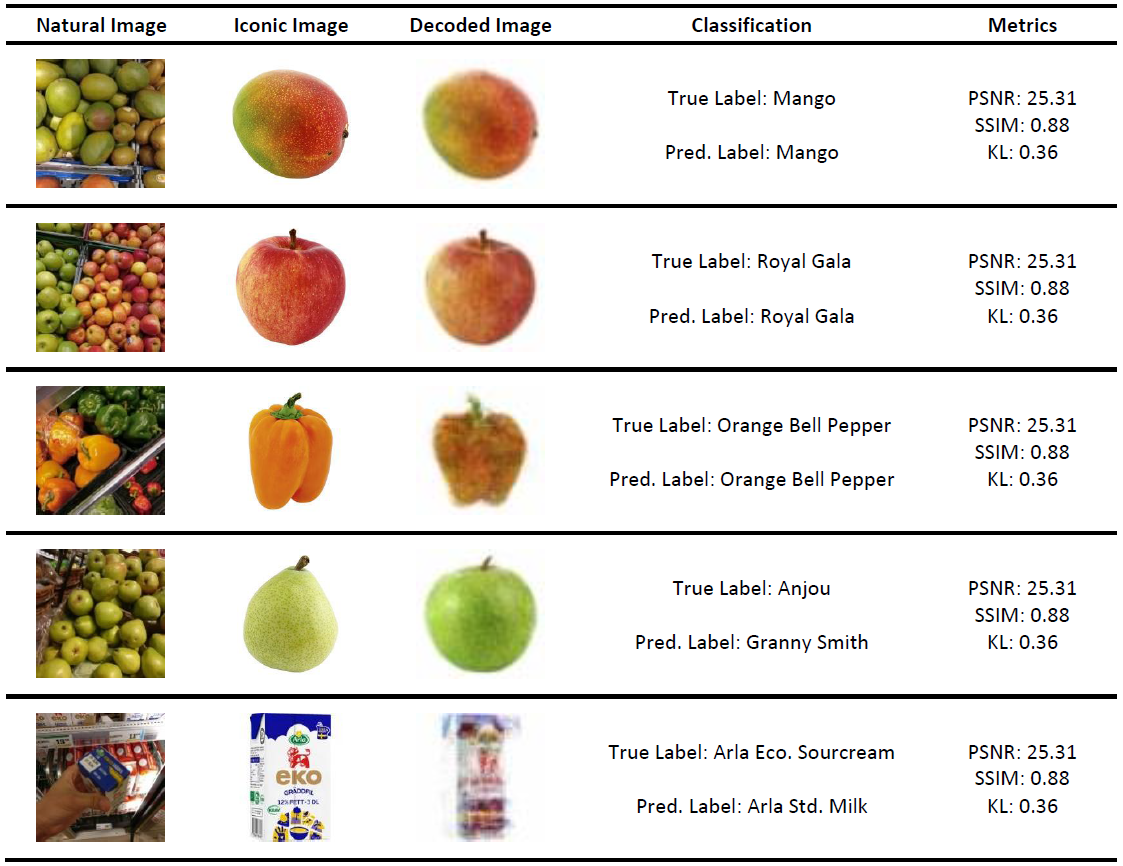
\includegraphics[width=0.95\textwidth]{PaperB/figures_and_tables/figure10.png}
    \vspace{-2mm}
    \caption{Examples of decoded iconic images from VCCA$_{xiwy}$ with their corresponding natural image and true iconic image as well as predicted labels and image similarity metrics. The column Classification shows the true label for the natural image (True Label) and the label predicted by the model (Pred. Label). %Abbreviations: VCCA, Variational Canonical Correlation Analysis; PSNR, Peak Signal-to-Noise Ratio; SSIM, Structural Similarity; KL, Kullback-Leibler Divergence; Arla Eco. Sourcream, Arla Ecological Sourcream; Arla Std. Milk, Arla Standard Milk.
    }
    \label{fig:decoded_iconic_images_with_metrics}
  	\vspace{-3mm}
\end{figure}

\section{Discussion}\label{paperB:sec:discussion}

In this section, we summarize the experimental results and discuss our findings.

\vspace{-3mm}
\paragraph{Classification Results} In the first experiments (see Section \ref{paperB:sec:classification_results}), %subsection Classification Results in Results),
%(Section \ref{sec:classification_results}), 
we showed that utilizing all four views with SplitAE$_{x i w y}$ and VCCA$_{x i w y}$ resulted in the best classification performance on the test set. This indicates that these models take advantage of each view to learn representations that enhance their generalization ability compared to the single-view models. Moreover, using either the iconic images, the text descriptions or both views yields better representations for classification compared to using the natural image features alone. Note that it was necessary to properly set the scaling weights $\lambda$ on the reconstruction losses of the additional views to achieve good classification performance (see Table S2).
Whenever the weight values are increased, the model tries to structure the representations according to variations between the items in the upweighted view rather than structuring the items based on visual features in the natural images, e.g., shape, color, and pose of items, image backgrounds, etc. 
Thus, the latent representations are structured based on semantic information that describes the item itself, which is important for constructing robust representations that generalize well in new environments. Furthermore, the class label decoders performed on par with the separate Softmax classifiers in most cases. The upside with training a separate classifier is that we only would have re-train the classifier if we receive a new class in the dataset, while we would have to train the whole model from scratch when the model uses a class label decoder. Note that the encoder for any of the multi-view models can be used for extracting latent representations for new tasks, whether the model utilizes the label or not, since the encoder only uses natural images as input. 

\vspace{-3mm}
\paragraph{Iconic Images vs. Text Descriptions} 
In Table \ref{tab:classification_results_on_test_set}, the iconic images yielded higher classification accuracies compared to using the text descriptions. This was also evident in Figure \ref{fig:varying_t} where the classification performance remains more or less the same regardless of the text description length $T$ when the models utilize iconic images. We believe that the main reasons for the advantages with iconic images lie in the clear visual features of the items in these images, e.g., their color and shape, which carry lots of information that is important for image classification tasks. However, we also observed that iconic images and text descriptions can yield different benefits for constructing good representations. In Figure \ref{fig:2d_visualizations_pca}, we see that iconic images and text descriptions make the model construct different latent representations of the grocery items. Iconic images structures the representations with respect to color and shape of the items (see Figure \ref{fig:2d_visualizations_pca_apples}), while the descriptions groups items based on their ingredients and flavor (see Figure \ref{fig:2d_visualizations_pca_juice_yoghurt}). Therefore, the latent representations benefit differently from utilizing the additional views and a combination of all of them yields the best classification performance as shown in Table \ref{tab:classification_results_on_test_set}. We want to highlight the results in Figure \ref{fig:2d_visualizations_pca_juice_yoghurt}, where the model manages to separate juice and yoghurt packages based on their text description. 
Refrigerated items, e.g., milk and juice packages, have in general very similar shapes and the same color if they come from the same brand.
There are minor visual differences between items of the same brand that makes it possible to differentiate between them, e.g., the picture of the main ingredient on the package and ingredient description. Additionally, these items can be almost identical depending on which side of the package that is present on the natural image. When utilizing the text descriptions, we add useful information on how to distinguish between visually similar items that have different ingredients and contents. This is highly important for using computer vision models to distinguish between packaged items without having to use other kinds of information, e.g., barcodes. 

\vspace{-3mm}
\paragraph{Text Description Length} We showed 
%in Section \ref{sec:classification_results} 
that the text descriptions are useful for the classification task, and that careful selection of the description length $T$ is important for achieving the best possible performance (see Section \ref{paperB:sec:classification_results}), %subsection Classification Results in Results). 
In Figure \ref{fig:varying_t}, we observed that most models achieve significantly better classification performance when the text description length $T$ increases up until $T=32$. The reason for this increase is due to the similarities between the descriptions of items from the same kind or brand, such as milk and juice packages. 
For instance, in Table S1, the first sentence in the descriptions for the milk packages only differ by the ninth word, which is \textit{organic} for the ecological milk package. 
This means that their descriptions will be identical when $T=8$. Therefore, the descriptions will become more different from each other as we increase $T$, which helps the model to distinguish between items with similar descriptions. However, the classification accuracies have more or less saturated when setting $T > 32$, which is also due to the similarity between the descriptions. For example, the bell pepper descriptions in Table S1 only differ by the second word that describes the color of the bell pepper, i.e., the words \textit{yellow} and \textit{orange}. We also see that the third and fourth sentences in the descriptions of the milk packages are identical. The text descriptions typically have words that separate the items in the first or second sentence, whereas the following sentences provide general information on ingredients and how the item can be used in cooking. For items of the same kind but of different colors or brand, e.g., bell peppers or milk packages respectively, the useful textual information for constructing good representations of grocery items typically comes from a few words in the description that describes features of the item. Therefore, the models yield better classification performance when $T$ is set to include at least the whole first sentence of the description. We could select $T$ more cleverly, e.g., by using different $T$ for different descriptions to make sure that we utilize the words that describe the item or filter out non-informative words for the classification task. 

\vspace{-3mm}
\paragraph{VCCA vs. VCCA-private} The main motivation for using VCCA-private is to use private latent variables for modeling view-specific variations, e.g., image backgrounds and writing styles of text descriptions. This could allow the model to build shared representations that more efficiently combine salient information shared between the views for training better classifiers. This would then remove noise from the shared representation since the private latent variables are responsible for modeling the view-specific variations. For VCCA-private$_{x w}$, we observed that the private latent spaces managed to group different image backgrounds and grocery items with similar text descriptions respectively in Figure \ref{fig:pca_vcca_private_xw_ux} and \ref{fig:pca_vcca_private_xw_uw} respectively. This model also performed on par with VCCA$_{x w}$ regarding classification performance in Table \ref{tab:classification_results_on_test_set}. However, we also saw in the same table that the VCCA-private models using the iconic image perform poorly on the classification task compared to their VCCA counterpart. The reason for why this model fails is because of a form of \textit{posterior collapse}~\citeB{B:bowman2015generating} in the encoder for the iconic image, where the encoder starts outputting random noise. We noticed this as the KL divergence term for the private latent variable converged to zero when we trained the models for 500 epochs (see Figure S2 and S3), which means that the encoder outputs a distribution which equals a Gaussian prior. The same phenomenon occurs for VCCA-private with the text description as well. We have also experimented with other models with encoders, such as Deep CCA and DCCAE, which also suffered from the collapsing encoder problem for the additional views. Therefore, we believe that the collapsing effect is a consequence of only having access to a single iconic image and text description for every grocery item. Therefore, a potential solution would be to extend the dataset with multiple web-scraped iconic images and text descriptions for every grocery item, which would then establish some variability within the view for each item class. Another possible solution would be to use data augmentation techniques to create some variability in the web-scraped views. For example, we could take a denoising approach and add noise to the iconic images which would force the decoder to reconstruct the real iconic images~\citeB{B:vincent2010stacked}. For the text descriptions, we could mask words at random in the encoder and let the decoder predict the whole description, which would work as a form of \textit{word dropout}~\citeB{B:bowman2015generating, B:devlin2018bert}. We leave this for future work if such augmentation techniques can create the needed variability for learning more robust representations as well as discovering the structures of the private latent spaces that this approach would bring. 

\vspace{-3mm}
\paragraph{Decoded Iconic Images} %In Section \ref{sec:decoding_iconic_images}, we 
We observed with image similarity metrics that the quality of decoded iconic images coheres to some extent with the classification performance for VCCA models using the iconic images (see Section \ref{paperB:sec:decoding_iconic_images}). %subsection Decoding Iconic Images from Unseen Natural Images in Results). 
We also showed that the decoded images are visually plausible decoded images with respect to colors, shapes, and identities of the grocery items in the dataset. The values for the metrics PSNR, SSIM, and KL divergence are similar across the different VCCA models. Since we used RGB values for estimating KL, we believe that including spatial information of pixels or using other color spaces, e.g., Lab, could provide more information about the dissimilarities between the decoded and true iconic images. To thoroughly assess the relationship between good classification performance and accurately decoding the iconic images, we also suggest evaluating the image quality on other image similarity metrics, e.g., perceptual similarity~\citeB{B:zhang2018unreasonable}. Finally, we see the decoding of iconic images as a promising method to evaluate the quality of the latent representations as well as enhancing the interpretability of the classification. For example, we could inspect decoded iconic images qualitatively or by using image similarity metrics to determine how certain the model was about the present items in the natural images, which could then be used as a tool for explaining misclassifications.

\subsection{Conclusions}
\label{paperB:sec:conclusions}

In this paper, we introduce a dataset with natural images of grocery items taken in real grocery store environments. Each item class is accompanied by web-scraped information in the form of an iconic image and a text description of the item. The main application for this dataset is for training image classifiers that can assist visually impaired people when shopping for groceries but is not limited to this use case only. 

We selected the multi-view generative model VCCA that can utilize all of the available data views for image classification. 
To evaluate the contribution to the classification performance for each view, we conducted an ablation study comparing classification accuracies between VCCA models with different combinations of the available data types. We showed that utilizing the additional views with VCCA yields higher accuracies on classifying grocery items over models only using the natural images.
The iconic images and text descriptions impose different structures of the shared latent space, where we observed that iconic images help to group the items based on their color and shape while text descriptions separate the items based on differences in ingredients and flavor.
These types of semantics that VCCA has learned can be useful for generalizing to new grocery items and other object recognition tasks. We also investigated VCCA-private, which introduces private latent variables for view-specific variations, that separates the latent space into shared and private spaces for each view to provide high-quality representations. However, we observed that the private latent variables for the web-scraped views became uninformative by modeling noise due to the lack of variations in the additional web-scraped views. This encourages to explore new methods for extracting salient information from such data views that can be beneficial for downstream tasks. 

An evident direction of future work would be to investigate other methods for utilizing the web-scraped views more efficiently. For instance, we could apply pre-trained word representations for the text description, e.g., BERT~\citeB{B:devlin2018bert} or GloVe~\citeB{B:pennington2014glove}, to see if they enable the construction of representations that can more easily distinguish between visually similar items. 
Another interesting direction would be to experiment with various data augmentation techniques in the web-scraped views to create view-specific variations without the need for collecting and annotating more data. It is also important to investigate how the model can be extended to recognize multiple items. Finally, we see zero- and few-shot learning~\citeB{B:xian2018zero} of new grocery items and transfer learning~\citeB{B:pan2010transferlearning} as potential applications where our dataset can be used for benchmarking of multi-view learning models on classification tasks. 
\section{Experimental Procedures}
\label{paperB:sec:experimental_procedures}

\subsection{Resource Availability}

\subsubsection{Lead Contact}
Marcus Klasson is the lead contact for this study and can be contacted by email at \url{mklas@kth.se}.

\subsubsection{Materials Availability}
There are no physical materials associated with this study.

\subsubsection{Data and Code Availability}
\begin{enumerate}
\item The Grocery Store dataset along with documentation is available at the following Github repository: \url{https://github.com/marcusklasson/GroceryStoreDataset}
\item The source code for the multi-view models along with documentation is available at the following Github repository: \url{https://github.com/marcusklasson/vcca_grocerystore}
\end{enumerate}

%In this section, we outline the details of all models that we use for grocery classification. We also provide a description of the experimental setups used to generate the results in Section \ref{sec:results}.

\subsection{Methods}\label{paperB:sec:methods}

In this section, we outline the details of the models we use for grocery classification.
We begin by introducing autoencoders and SplitAEs~\citeB{B:wang2015deep}. Then we describe VAEs~\citeB{B:kingma2013auto} and how it is applied to single-view data, followed by the introduction of VCCA~\citeB{B:wang2016deep} and how we adapt it to our dataset. We also discuss a variant of VCCA called VCCA-private~\citeB{B:wang2016deep}, which is used for extracting private information about each view in addition to shared information across all views by factorizing the latent space. The graphical model representations of the VAE, VCCA, and VCCA-private models that have been used in this paper are shown in Figure S5. The model names use subscripts to denote the views utilized for learning the shared latent representations. For example, VCCA$_{x i}$ utilizes natural image features $x$ and iconic images $i$, while VCCA$_{x i w y}$ uses natural image features $x$ and iconic images $i$, text descriptions $w$, and class labels $y$.

\subsubsection{Autoencoders and Split Autoencoders}
\label{paperB:sec:autoencoders_and_split_autoencoders}

The autoencoding framework can be used for feature extraction and learning latent representations of data in unsupervised manners~\citeB{B:bengio2013representation}. It begins with defining a parameterized function called the encoder for extracting features. We denote the encoder as $f_{\phi}$ where $\phi$ includes its parameters, which commonly are the weights and bias vectors of a neural network. The encoder is used for computing a feature vector $h = f_{\phi}(x)$ from the input data $x$. Another parameterized function $g_{\theta}$ called the decoder is also defined, that maps the feature $h$ back into input space, i.e., $\hat{x} = g_{\theta}(h)$. The encoder and decoder are learned simultaneously to minimize the reconstruction loss between the input and its reconstruction of all training samples. By setting the dimension of the feature vector smaller than the input dimension, i.e., $d_{h} < d_{x}$, the autoencoder can be used for dimensionality reduction which makes the feature vectors suitable for training linear classifiers in a cheap way.

As in the case for the Grocery Store dataset, we have multiple views available during training, while only the natural image view is present at test time. In this setting, we can use a Split Autoencoder (SplitAE) to extract shared representations by reconstructing all views during training from the one view that is available during the test phase~\citeB{B:ngiam2011multimodal, B:wang2015deep}. As an example, we have the two-view case with $x$ present at both training and test while $y$ is only available during training. We therefore define an encoder $f_{\phi}$ and two decoders $g_{\theta_{x}}$ and $g_{\theta_{y}}$ where both decoders inputs the same representation $h = f_{\phi}(x)$. The objective of the SplitAE is to minimize the sum of the reconstruction losses, which will encourage representations $h$ that best reconstructs both views. The total loss is then 
\begin{align}\label{eq:splitae_objective}
    \mathcal{L}_{SplitAE}(\theta, \phi; x, y) = \lambda_{x} \mathcal{L}_{x}(x, g_{\theta_{x}}(h)) + \lambda_{y} \mathcal{L}_{y}(y, g_{\theta_{y}}(h)) ,
\end{align}
where $\theta_{x}, \theta_{y} \in \theta$ and $\lambda_{x}, \lambda_{y}$ are scaling weights for the reconstruction losses.
For images, the reconstruction loss can be the mean squared error, while the cross-entropy loss is commonly used for class labels and text. This architecture can be extended to more than two views by simply using view-specific decoders that input the shared representation extracted from natural images. Note that in the case when the class labels are available, we can use the class label decoder $g_{\theta_{y}}$ as a classifier during test time. Alternatively, we can train a separate classifier with the learned shared representations after the SplitAE has been trained.


\subsubsection{Variational Autoencoders with only Natural Images}
\label{paperB:sec:vae_with_only_natural_images}
The Variational Autoencoder (VAE) is a generative model that can be used for generating data from single views. Here, we describe how the VAE learns latent representations of the data and how the model can be used for classification.
VAEs define a joint probability distribution $p_{\theta}(x,z) = p(z) p_{\theta}(x|z)$, where $p(z)$ is a prior distribution over the latent variables $z$ and $p_{\theta}(x|z)$ is the likelihood over the natural images $x$ given $z$. The prior distribution is often assumed to be an isotropic Gaussian distribution, $p(z) = \mathcal{N}(z\,|\, \boldsymbol{0}, \mathbf{I})$, with the zero vector $\boldsymbol{0}$ as mean and the identity matrix $\mathbf{I}$ as the covariance.  
The likelihood $p_{\theta}(x|z)$ takes the latent variable $z$ as input and outputs a distribution parameterized by a neural network with parameters $\theta$
which is referred to as the decoder network.
A common distribution for natural images is a multivariate Gaussian, $p_{\theta}(x|z) = \mathcal{N}(x\,|\, \mu_{x}(z), \bm{\sigma}_{x}^2(z) \odot \mathbf{I})$, where $\mu_{x}(z)$ and $\bm{\sigma}_{x}^2(z)$ are the means and standard deviations of the pixels respectively outputted from the decoder and $\odot$ denotes element-wise multiplication. 
We wish to find latent variables $z$ that are likely to have generated $x$, which is done by approximating the intractable posterior distribution $p_{\theta}(z|x)$ with a simpler distribution $q_{\phi}(z|x)$~\citeB{B:zhang2018advances}. This approximate posterior $q_{\phi}(z|x)$ is referred to as the encoder network since it is parameterized by a neural network $\phi$ which inputs $x$ and outputs a latent variable $z$. Commonly, we let the approximate posterior to be Gaussian
$q_{\phi}(z|x) = \mathcal{N}(z \,|\,\mu_{z}(x), \sigma_{z}^2(x) \odot \mathbf{I})$, where the mean $\mu_{z}(x)$ and variance $\sigma_{z}^2(x)$ are the outputs of the encoder. The latent variable $z$ is then sampled using the mean and variance from the encoder with the reparameterization trick~\citeB{B:kingma2013auto,B:rezende2014stochastic}. The goal is to maximize a tractable lower bound on the marginal log-likelihood of $x$ using $q_{\phi}(z|x)$:
\begin{align}
\begin{split}\label{eq:vae-loss}
\log p_{\theta}(x) \geq \, \mathcal{L}(\theta, \phi; x) = \, \E_{q_{\phi}(z|x)}\left[\, \log p_{\theta}(x | z) \,\right]  -\KL(q_{\phi}(z|x)\,||\,p(z)) .
\end{split}
\end{align}
The last term is the Kullback-Leibler (KL) divergence~\citeB{B:kullback1951information} of the approximate posterior from the prior distribution, which can be computed analytically when $q_{\phi}(z|x)$ and $p(z)$ are Gaussians. The expectation can be viewed as a reconstruction loss term, which can be approximated using Monte Carlo sampling from $q_{\phi}(z|x)$. The lower bound $\mathcal{L}$ is called the evidence lower bound (ELBO) and can be optimized with stochastic gradient descent via backpropagation. The mean outputs $\mu_{z}(x)$ from the encoder $q_{\phi}(z|x)$ are commonly used as the latent representation of the natural images $x$. We can use the representations
$\mu_{z}(x)$ for training any classifier $p(y | \mu_{z}(x))$, e.g., a Softmax classifier, where $y$ is the class label of $x$. We can therefore see training the VAE as a pre-processing step, where we extract a lower-dimensional representation of the data $x$ which hopefully makes the classification problem easier to solve. 
We can also extend the VAE with a generative classifier by incorporating the class label $y$ in the model~\citeB{B:li2019generative, B:ma2018eddi}. 
Hence, the VAE defines a joint distribution $p_{\theta}(x, y, z) = p(z) p_{\theta_{x}}(x|z) p_{\theta_{y}}(y|z)$ where the class label decoder $p_{\theta_{y}}(y|z)$ is used as the final classifier. 
We therefore aim to maximize the ELBO on the marginal log-likelihood over $x$ and $y$: 
\begin{align}\label{eq:loss_vcca_xy}
    \begin{split}
        \log p_{\theta}(x, y) \geq & \, \mathcal{L}(\theta, \phi; x, y) \\ 
        = & \,  \lambda_{x} \E_{q_{\phi}(z|x)}\left[\, \log p_{\theta_{x}}(x | z) \right] + \lambda_{y} \E_{q_{\phi}(z|x)}\left[\, \log p_{\theta_{y}}(y | z) \,\right] - \KL(q_{\phi}(z|x)\,||\,p(z)) .
    \end{split}
\end{align}  
The parameters $\lambda_{x}$ and $\lambda_{y}$ are used for scaling the magnitudes of the expected values. When predicting the class label for an unseen natural image $x^{*}$, we can consider multiple output predictions of the class label by sampling $K$ different latent variables for $x^{*}$ from the encoder to determine the final predicted class. For example, we could either average the predicted class scores over $K$ or use the maximum class score from $K$ samples as the final predictions. In this paper, we compute the average of the predicted class scores using
\begin{align}\label{eq:prediction_vcca_xy}
    \hat{y} = \argmax_{y} \frac{1}{K} \sum_{k=1}^{K} p_{\bm{\theta_{y}}}(y | z^{(k)}), \,\, z^{(k)} \sim q_{\phi}(z | x^{*}) ,
\end{align}
where $\hat{y}$ is the predicted class for the natural image $x^{*}$. We denote this model as VCCA$_{x y}$ due to its closer resemblance to VCCA than VAE in this paper.


\subsubsection{Variational Canonical Correlation Analysis for Utilizing Multi-View Data}
\label{paperB:sec:utilizing_additional_information}

In this section, we describe the details of Variational Canonical Correlation Analysis (VCCA)~\citeB{B:wang2016deep} for our application. In the Grocery Store dataset, the views can be the natural images, iconic images, text descriptions, or class labels and we can use any combination of those three in VCCA. To illustrate how we can employ this model to the Grocery Store dataset, we let the natural images $x$ and the iconic images $i$ be the two views.  
We assume that both views $x$ and $i$ have been generated from a single latent variable $z$. Similarly as with VAEs, VCCA defines a joint probability distribution $p_{\theta}(x, i, z) = p(z)p_{\theta_{x}}(x\,|\,z)p_{\theta_{i}}(i\,|\,z)$. There are now two likelihoods for each view modeled by the decoders $p_{\theta_{x}}(x\,|\,z)$ and $p_{\theta_{i}}(i\,|\,z)$ are represented as neural networks with parameters $\theta_{x}$ and $\theta_{i}$. 
Since we want to classify natural images, the other available views in the dataset will be missing when we have received a new natural image. Therefore, the encoder $\vq_{\phi}(z | x)$ only uses $x$ as input to infer the latent variable $z$ shared across all views, such that we do not have to use inference techniques that handle missing views. With this choice of approximate posterior, we receive the following ELBO on the marginal log-likelihood over $x$ and $i$ that we aim to maximize:
\begin{align}\label{eq:loss_vcca}
    \begin{split}
        \log p_{\theta}(x, i) \geq & \, \mathcal{L}(\theta, \phi; x, i) \\ 
        = & \,  \lambda_{x} \E_{q_{\phi}(z|x)}\left[\, \log p_{\theta_{x}}(x | z) \right] + \lambda_{i} \E_{q_{\phi}(z|x)}\left[\, \log p_{\theta_{i}}(i | z) \,\right] - \KL(q_{\phi}(z|x)\,||\,p(z)) .
    \end{split}
\end{align}  
The parameters $\lambda_{x}$ and $\lambda_{i}$ are used for scaling the magnitude of the expected values for each view. 
We provide a derivation of the ELBO for three or more views in the Supplemental Experimental Procedures.
%supplementary material.
The representations $\mu_{z}(x)$ from the encoder $q_{\phi}(z|x)$ can be used for training a separate classifier. We can also add a class label decoder $p_{\theta_{y}}(y | z)$ to the model and use Equation \ref{eq:prediction_vcca_xy} to predict the class of unseen natural images.


\subsubsection{Extracting Private Information of Views with VCCA-private}
\label{paperB:sec:extracting_private_information}

In the following section, %discussion,
we show how the VCCA model can be altered to extract shared information between the views as well as view-specific private information to enable more efficient posterior inference.
Assuming that a shared latent variable $z$ is sufficient for generating all different views may have its disadvantages. Since the information in the views is rarely fully independent nor fully correlated, information only relevant to one of the views will be mixed with the shared information. This may complicate the inference of the latent variables, which potentially can harm the classification performance. To tackle this problem, previous works have proposed learning separate latent spaces for modeling shared and private information of the different views~\citeB{B:salzmann2010factorized, B:wang2016deep, B:zhang2016inter}. The shared information should represent the correlations between the views, while the private information represents the independent variations within each view. 
As an example, 
the shared information between natural and iconic images are the visual features of the grocery item, while their private information is considered as the various backgrounds that can appear in the natural images and the different locations of non-white pixels in the iconic images. For the text descriptions, the shared information would be words that describe visual features in the natural images, whereas the private information would be different writing styles for describing grocery items with text.   
We adapt the approach from~\citeB{B:wang2016deep} called VCCA-private and introduce private latent variables for each view along with the shared latent variable.
To illustrate how we employ this model to the Grocery Store dataset, we let the natural images $x$ and the text descriptions $w$ be the two views. The joint distribution of this model is written as 
\begin{align}
    p_{\theta}(x, w, z, u_{x}, u_{w}) = p_{\theta_{x}}(x | z, u_{x}) p_{\theta_{w}}(w | z, u_{w}) p(z) p(u_{x}) p(u_{w}) ,
\end{align}
where $u_{x}$ and $u_{w}$ are the private latent variables for the $x$ and $w$ respectively. To enable tractable inference of this model, we employ a factorized approximate posterior distribution of the form
\begin{align}\label{eq:vcca_private_approximate_posterior}
    q_{\phi}(z, u_{x}, u_{w} | x, w) = q_{\phi_{z}}(z | x) q_{\phi_{x}}(u_{x} | x) q_{\phi_{w}}(u_{w} | w),
\end{align}
where each factor is represented as an encoder network inferring its associated latent variable. With this approximate posterior, the ELBO for VCCA-private is given by
\begin{align}
    \begin{split} \label{eq:loss_vcca_private_xw}
        \log p_{\theta}(x, w) \geq & \, \mathcal{L}_{\text{private}}(\theta, \phi; x, w) \\ 
        = & \, \lambda_{x} \E_{q_{\phi_{z}}(z|x), q_{\phi_{x}}(u_{x}|x)}\left[\, \log p_{\theta_{x}}(x | z, u_{x}) \right] + \lambda_{w}  \E_{q_{\phi_{z}}(z|x), q_{\phi_{w}}(u_{w}|w)}\left[\, \log p_{\theta_{w}}(w | z, u_{w}) \right] \\ 
        & - \KL(q_{\phi_{z}}(z|x)\,||\,p(z)) - \KL(q_{\phi_{x}}(u_{x}|x)\,||\,p(u_{x})) - \KL(q_{\phi_{w}}(u_{w} |w)\,||\,p(u_{w})) .
    \end{split}
\end{align}
The expectations in $\mathcal{L}_{\text{private}}(\theta, \phi; x, w)$ in Equation \ref{eq:loss_vcca_private_xw} can be approximated using Monte Carlo sampling from $q_{\phi}(z | x)$. The sampled latent variables are concatenated and then used as input to their corresponding decoder. We let the approximated posteriors over both shared and private latent variables to be multivariate Gaussian distributions and their priors distributions to be standard isotropic Gaussians $\mathcal{N}(\bm{0}, \mathbf{I})$. The KL divergences in Equation \ref{eq:vcca_private_approximate_posterior} can then be computed analytically. 
Since only natural images are present during test time and because the shared latent variable $z$ since it should contain information about similarities between the views, e.g., the object class, we use the encoder $q_{\phi}(z|x)$ to extract latent representations $\mu_{z}(x)$ for training a separate classifier. As for the VAE and standard VCCA, we can also add a class label decoder $p_{\theta_{y}}(y | z)$ only conditioned on $z$ to the model and use Equation \ref{eq:prediction_vcca_xy} to predict the class of unseen natural images. We evaluated the classification performance of VCCA-private and compare it to the standard VCCA model only using a single shared latent variable (see subsection Classification Results in Result). %In Section \ref{sec:classification_results}, we evaluate the classification performance of VCCA-private and compare it to the standard VCCA model only using a single shared latent variable. 


\subsection{Experimental Setup}
\label{paperB:sec:experimental_setup}

This section briefly describes the network architecture designs and the selection of hyperparameters for the models. See the Supplemental Experimental Procedures
%supplementary material 
for full details on the network architectures and hyperparameters that we use.

\paragraph{Processing of Natural Images} We use a DenseNet169~\citeB{B:huang2017densely} as the backbone for processing the natural images since this architecture showed good classification performance in~\citeB{B:klasson2019hierarchical}. As our first baseline, we customize the output layer of DenseNet169 to our the Grocery Store dataset and train it from scratch to classify the natural images. For the second baseline, we train a Softmax classifier on off-the-shelf features from DenseNet169 pre-trained on the ImageNet dataset~\citeB{B:deng2009imagenet}, where we extract 1664-dimensional from the average pooling layer before the classification layer in the architecture. Using pre-trained networks as feature extractors for smaller datasets has previously been proven to be a successful approach for classification tasks~\citeB{B:razavian2014cnnfeatures}, which makes it a suitable baseline for the Grocery Store dataset. We denoted the DenseNet169 trained from scratch and the Softmax classifier trained on off-the-shelf features as DenseNet-scratch and Softmax respectively in the Results section.%We denote the DenseNet169 trained from scratch and the Softmax classifier trained on off-the-shelf features as DenseNet-scratch and Softmax respectively in the further sections.

\paragraph{Network Architectures} We use the same architectures for SplitAE and VCCA for a fair comparison. We train the models using off-the-shelf features extracted from a pre-trained DenseNet169 for the natural images. No fine-tuning of the DenseNet backbone was used in the experiments, which we leave for future research. The image feature encoder and decoder consist of a single hidden layer, where the encoder outputs the latent representation and the decoder reconstructs the image feature. We use a DCGAN~\citeB{B:radford2015unsupervised} generator architecture for the iconic image decoder reconstructing the iconic images. The text description is predicted sequentially using an LSTM network~\citeB{B:hochreiter1997long}. The label decoder uses a single hidden layer with 512 hidden units and Leaky ReLU activation. 
The latent space dimension to $d_{z} = 200$ for all SplitAE and VCCA models in the experiments. In the VCCA-private models, the encoder and decoders have the same architectures as in the VCCA models. We use a reversed DCGAN generator as the iconic image encoder. The text description encoder is an LSTM. We obtain an embedding for the description by averaging all of the hidden states $h_t$ generated from the LSTM, i.e., $\frac{1}{T} \sum_{t=1}^{T} h_t$, and input it to a linear layer that outputs the latent representation. The dimensions of the private latent spaces are the same as the shared latent space dimension $d_{z} = 200$. 

\paragraph{Training Details} In all experiments, we train all models for 200 epochs using the Adam optimizer~\citeB{B:kingma2015adam} with initial learning rate $10^{-4}$ and hyperparameters $\beta_1 = 0.9$ and $\beta_2 = 0.999$. We apply the sum-of-squares loss for the natural and iconic images and the categorical cross-entropy loss for text descriptions and class labels. The latent representations for the AE and SplitAE are the output from the encoder, while for the VAE, VCCA, and VCCA-private we instead use the mean outputs $\mu_{z}(x)$ from the encoder. In VCCA-private, we use the the mean outputs $\mu_{u_{x}}(x)$ and $\mu_{u_{w}}(w)$ for visualizing the private latent representations (see Figure \ref{fig:2d_visualizations_pca_vcca_private_xw}). The Softmax classifiers are trained for 100 epochs using with initial learning rate $10^{-4}$ and hyperparameters $\beta_1 = 0.5$ and $\beta_2 = 0.999$. We run a hyperparameter search for the scaling weights $\lambda$ for the reconstruction losses of each view (see the Supplemental Experimental Procedures
%supplementary material 
for more details). 

\paragraph{Choice of Text Description Length $T$} We wanted to investigate how the classification performance is affected by the text description length $T$ for the SplitAE and VCCA models using the text description $w$. Since the LSTM predicts the text description sequentially, the computational time increases as the text description length increases. We began by setting $T = 16$ because of how the sentence length was set for the image captioning model in \citeB{B:lu2018neural}. Then we created an interval by taking steps with 8 words up to $T=40$ and included the minimum, mean, and maximum text description lengths which are $T=6, 36$, and $91$ respectively. We added two additional points at $T=50$ and $75$ since for most models there was a slight increase in classification performance when $T$ was increased from $40$ to $91$. 

\paragraph{Computational Time} The computational time for the SplitAE and VCCA models differs depending on which views that are being used. We measured the number of seconds per epoch (s/epoch) on an Nvidia GeForce RTX 2080 Ti, where an epoch consists of the 2640 training samples. Running experiments with the text description view 
%, i.e., VCCA$_{x w}$ and VCCA$_{x w y}$,
took around 0.4--2.7 s/epoch with text description length $T \in [6, 91]$. Adding the iconic image view and training the models 
% VCCA$_{x i w}$ and VCCA$_{x i w y}$ 
took around 4.5--6.2 s/epoch depending on the text description length.


\paragraph{Visualization Method} We use PCA to visualize the latent space by plotting the latent representations from the trained encoders. PCA is used for projecting the representations from dimension $d_{z}$ to a 2D space. We obtain the principal components for the representations with the natural images from the training set. In all figures, we plot the representations of test set images given the principal components obtained from the training images (see subsection Investigation of the Learned Representations in Results). To distinguish more easily between the class labels of the images, we occasionally use the iconic images from the dataset and plot the corresponding iconic image of the representation on its location in the 2D space.



%\clearpage
\section*{Acknowledgments}
This research is funded by the Promobilia foundation and the Swedish
e-Science Research Centre.

%\renewcommand*{\bibname}{References}
\bibliographystyleB{unsrt}
{\small
	\bibliographyB{PaperB/refB}
}

\begin{appendices}
	\renewcommand{\thesection}{\Roman{section}}
	

\section{Supplemental Figures}
\label{paperB:supp:supplemental_figures}


\begin{figure}[h!]
	\centering
	\resizebox{0.8\textwidth}{!}{
		\begin{minipage}[t]{\textwidth}
			%\centering
			\begin{subfigure}[t]{0.21\textwidth}
				\centering
				% model_lda.tex
%
% Copyright (C) 2010,2011 Laura Dietz
% Copyright (C) 2012 Jaakko Luttinen
%
% The MIT License
%
% See LICENSE file for more details.

% Latent Diriclet allocation model
\tikzstyle{obs}=[circle,draw=black!50,fill=gray!25,thick,inner sep=0pt,minimum size=6mm]
\tikzstyle{latent}=[circle,draw=black!50,thick,inner sep=0pt,minimum size=6mm]
\tikzstyle{solid}=[draw=black!50, thick, >=stealth]

% Had to add ghost node because caption VAE_x didn't fit on one line...
\tikzstyle{ghost}=[circle,draw=white,thick,inner sep=0pt,minimum size=4mm]

\begin{tikzpicture}[x=1.cm,y=1.cm]

  % Nodes
  \node[obs]                    (x)    {$x$} ; %
  \node[ghost, right=0.1cm of x] (ghost1) {};
  \node[ghost, left=0.1cm of x] (ghost2) {};
  \node[latent, above=of x]    (z)     {$z$} ; %
  
  % Factors
  % Connect nodes
  \edge [solid] {z} {x} ; %

\end{tikzpicture}


				%\includegraphics[width=\textwidth]{PaperB/appendix/figures/tikz_figures/vae_x}
				\caption{VAE$_{x}$}
				\label{fig:tikz_vae_x}
			\end{subfigure} \hspace{2mm}
			\begin{subfigure}[t]{0.21\textwidth}
				\centering
				% model_lda.tex
%
% Copyright (C) 2010,2011 Laura Dietz
% Copyright (C) 2012 Jaakko Luttinen
%
% The MIT License
%
% See LICENSE file for more details.

% Latent Diriclet allocation model

\tikzstyle{obs}=[circle,draw=black!50,fill=gray!25,thick,inner sep=0pt,minimum size=6mm]
\tikzstyle{latent}=[circle,draw=black!50,thick,inner sep=0pt,minimum size=6mm]
\tikzstyle{solid}=[draw=black!50, thick, >=stealth]

\begin{tikzpicture}[x=1.cm,y=1.cm]

  % Nodes
  \node[obs]                    (x)    {$x$} ; %
  \node[obs, right=1.0cm of x]  (y)    {$y$} ; %
  \node[latent, above right=1.2cm and .4cm of x]    (z)     {$z$} ; %
  
  % Factors
  % Connect nodes
  \edge [solid] {z} {x} ; %
  \edge [solid] {z} {y} ; %

\end{tikzpicture}


				%\includegraphics[width=\textwidth]{PaperB/appendix/figures/tikz_figures/vae_x}
				\caption{VCCA$_{x y}$}
				\label{fig:tikz_vcca_xy}
			\end{subfigure} \hspace{2mm}
			\begin{subfigure}[t]{0.21\textwidth}
				\centering
				% model_lda.tex
%
% Copyright (C) 2010,2011 Laura Dietz
% Copyright (C) 2012 Jaakko Luttinen
%
% The MIT License
%
% See LICENSE file for more details.

% Latent Diriclet allocation model

\tikzstyle{obs}=[circle,draw=black!50,fill=gray!25,thick,inner sep=0pt,minimum size=6mm]
\tikzstyle{latent}=[circle,draw=black!50,thick,inner sep=0pt,minimum size=6mm]
\tikzstyle{solid}=[draw=black!50, thick, >=stealth]

\begin{tikzpicture}[x=1.cm,y=1.cm]

  % Nodes
  \node[obs]                    (x)    {$x$} ; %
  \node[obs, right=1.cm of x]  (i)    {$i$} ; %
  \node[latent, above right=1.2cm and .4cm of x]    (z)     {$z$} ; %
  
  % Factors
  % Connect nodes
  \edge [solid] {z} {x} ; %
  \edge [solid] {z} {i} ; %

\end{tikzpicture}


				%\includegraphics[width=\textwidth]{PaperB/appendix/figures/tikz_figures/vae_x}
				\caption{VCCA$_{x i}$}
				\label{fig:tikz_vcca_xi}
			\end{subfigure} \hspace{2mm}
			\begin{subfigure}[t]{0.21\textwidth}
				\centering
				% model_lda.tex
%
% Copyright (C) 2010,2011 Laura Dietz
% Copyright (C) 2012 Jaakko Luttinen
%
% The MIT License
%
% See LICENSE file for more details.

% Latent Diriclet allocation model

\tikzstyle{obs}=[circle,draw=black!50,fill=gray!25,thick,inner sep=0pt,minimum size=6mm]
\tikzstyle{latent}=[circle,draw=black!50,thick,inner sep=0pt,minimum size=6mm]
\tikzstyle{solid}=[draw=black!50, thick, >=stealth]

\begin{tikzpicture}[x=1.cm,y=1.cm]

  % Nodes
  \node[obs]                    (x)    {$x$} ; %
  \node[obs, right=0.45cm of x]  (i)    {$i$} ; %
  \node[obs, right=0.45cm of i]  (y)    {$y$} ; %
  \node[latent, above= of i]    (z)     {$z$} ; %
  
  % Factors
  % Connect nodes
  \edge [solid] {z} {x} ; %
  \edge [solid] {z} {y} ; %
  \edge [solid] {z} {i} ; %

\end{tikzpicture}


				%\includegraphics[width=\textwidth]{PaperB/appendix/figures/tikz_figures/vae_x}
				\caption{VCCA$_{x i y}$}
				\label{fig:tikz_vcca_xiy}
			\end{subfigure} 
			\\[3mm]
			\begin{subfigure}[t]{0.20\textwidth}
				\centering
				% model_lda.tex
%
% Copyright (C) 2010,2011 Laura Dietz
% Copyright (C) 2012 Jaakko Luttinen
%
% The MIT License
%
% See LICENSE file for more details.

% Latent Diriclet allocation model

\tikzstyle{obs}=[circle,draw=black!50,fill=gray!25,thick,inner sep=0pt,minimum size=6mm]
\tikzstyle{latent}=[circle,draw=black!50,thick,inner sep=0pt,minimum size=6mm]
\tikzstyle{solid}=[draw=black!50, thick, >=stealth]

\begin{tikzpicture}[x=1.cm,y=1.cm]

  % Nodes
  \node[obs]                    (x)    {$x$} ; %
  \node[obs, right=1.cm of x]  (w)    {$w$} ; %
  \node[latent, above right=1.2cm and .4cm of x]    (z)     {$z$} ; %
  
  % Factors
  % Connect nodes
  \edge [solid] {z} {x} ; %
  \edge [solid] {z} {w} ; %

\end{tikzpicture}


				\caption{VCCA$_{x w}$}
				\label{fig:tikz_vcca_xw}
			\end{subfigure} \hspace{2mm}
			\begin{subfigure}[t]{0.20\textwidth}
				\centering
				% model_lda.tex
%
% Copyright (C) 2010,2011 Laura Dietz
% Copyright (C) 2012 Jaakko Luttinen
%
% The MIT License
%
% See LICENSE file for more details.

% Latent Diriclet allocation model

\tikzstyle{obs}=[circle,draw=black!50,fill=gray!25,thick,inner sep=0pt,minimum size=6mm]
\tikzstyle{latent}=[circle,draw=black!50,thick,inner sep=0pt,minimum size=6mm]
\tikzstyle{solid}=[draw=black!50, thick, >=stealth]

\begin{tikzpicture}[x=1.cm,y=1.cm]

  % Nodes
  \node[obs]                    (x)    {$x$} ; %
  \node[obs, right=0.45cm of x]  (w)    {$w$} ; %
  \node[obs, right=0.45cm of w]  (y)    {$y$} ; %
  \node[latent, above= of w]    (z)     {$z$} ; %
  
  % Factors
  % Connect nodes
  \edge [solid] {z} {x} ; %
  \edge [solid] {z} {y} ; %
  \edge [solid] {z} {w} ; %

\end{tikzpicture}


				%\includegraphics[width=\textwidth]{PaperB/appendix/figures/tikz_figures/vae_x}
				\caption{VCCA$_{x w y}$}
				\label{fig:tikz_vcca_xwy}
			\end{subfigure} \hspace{2mm}
			\begin{subfigure}[t]{0.20\textwidth}
				\centering
				% model_lda.tex
%
% Copyright (C) 2010,2011 Laura Dietz
% Copyright (C) 2012 Jaakko Luttinen
%
% The MIT License
%
% See LICENSE file for more details.

% Latent Diriclet allocation model

\tikzstyle{obs}=[circle,draw=black!50,fill=gray!25,thick,inner sep=0pt,minimum size=6mm]
\tikzstyle{latent}=[circle,draw=black!50,thick,inner sep=0pt,minimum size=6mm]
\tikzstyle{solid}=[draw=black!50, thick, >=stealth]

\begin{tikzpicture}[x=1.cm,y=1.cm]

  % Nodes
  \node[obs]                    (x)    {$x$} ; %
  \node[obs, right=0.45cm of x]  (i)    {$i$} ; %
  \node[obs, right=0.45cm of i]  (w)    {$w$} ; %
  \node[latent, above= of i]    (z)     {$z$} ; %
  
  % Factors
  % Connect nodes
  \edge [solid] {z} {x} ; %
  \edge [solid] {z} {i} ; %
  \edge [solid] {z} {w} ; %

\end{tikzpicture}


				%\includegraphics[width=\textwidth]{PaperB/appendix/figures/tikz_figures/vae_x}
				\caption{VCCA$_{x i w}$}
				\label{fig:tikz_vcca_xiw}
			\end{subfigure} \hspace{2mm}
			\begin{subfigure}[t]{0.20\textwidth}
				\centering
				% model_lda.tex
%
% Copyright (C) 2010,2011 Laura Dietz
% Copyright (C) 2012 Jaakko Luttinen
%
% The MIT License
%
% See LICENSE file for more details.

% Latent Diriclet allocation model

\tikzstyle{obs}=[circle,draw=black!50,fill=gray!25,thick,inner sep=0pt,minimum size=6mm]
\tikzstyle{latent}=[circle,draw=black!50,thick,inner sep=0pt,minimum size=6mm]
\tikzstyle{solid}=[draw=black!50, thick, >=stealth]

\begin{tikzpicture}[x=1.cm,y=1.cm]

  % Nodes
  \node[obs]                    (x)    {$x$} ; %
  \node[obs, right=0.3cm of x]  (i)    {$i$} ; %
  \node[obs, right=0.3cm of i]  (w)    {$w$} ; %
  \node[obs, right=0.3cm of w]  (y)    {$y$} ; %
  \node[latent, above right=1.2cm and .05cm of i]    (z)     {$z$} ; %
  
  % Factors
  % Connect nodes
  \edge [solid] {z} {x} ; %
  \edge [solid] {z} {i} ; %
  \edge [solid] {z} {w} ; %
  \edge [solid] {z} {y} ; %

\end{tikzpicture}


				%\includegraphics[width=\textwidth]{PaperB/appendix/figures/tikz_figures/vae_x}
				\caption{VCCA$_{x i w y}$}
				\label{fig:tikz_vcca_xiwy}
			\end{subfigure}
			\\[3mm]
			\begin{subfigure}[t]{0.21\textwidth}
				\centering
				% model_lda.tex
%
% Copyright (C) 2010,2011 Laura Dietz
% Copyright (C) 2012 Jaakko Luttinen
%
% The MIT License
%
% See LICENSE file for more details.

% Latent Diriclet allocation model

\tikzstyle{obs}=[circle,draw=black!50,fill=gray!25,thick,inner sep=0pt,minimum size=6mm]
\tikzstyle{latent}=[circle,draw=black!50,thick,inner sep=0pt,minimum size=6mm]
\tikzstyle{solid}=[draw=black!50, thick, >=stealth]

\begin{tikzpicture}[x=1.cm,y=1.cm]

  % Nodes
  \node[obs]                    (x)    {$x$} ; %
  %\node[obs, right=0.45cm of x]  (y)    {$\vy$} ; %
  \node[obs, right=1.2cm of x]  (i)    {$i$} ; %
  \node[latent, above= of x]    (ux)     {$u_{x}$} ; %
  \node[latent, right=0.3cm of ux]    (z)     {$z$} ; %
  \node[latent, right= 0.3cm of z]    (ui)     {$u_{i}$} ; %
  
  % Factors
  % Connect nodes
  \edge [solid] {z} {x} ; %
  \edge [solid] {z} {i} ; %
  \edge [solid] {ux} {x} ; %
  \edge [solid] {ui} {i} ; %

\end{tikzpicture}


				\caption{VCCA-private$_{x i}$}
				\label{fig:tikz_vcca_private_xi}
			\end{subfigure} \hspace{2mm}
			\begin{subfigure}[t]{0.21\textwidth}
				\centering
				% model_lda.tex
%
% Copyright (C) 2010,2011 Laura Dietz
% Copyright (C) 2012 Jaakko Luttinen
%
% The MIT License
%
% See LICENSE file for more details.

% Latent Diriclet allocation model

\tikzstyle{obs}=[circle,draw=black!50,fill=gray!25,thick,inner sep=0pt,minimum size=6mm]
\tikzstyle{latent}=[circle,draw=black!50,thick,inner sep=0pt,minimum size=6mm]
\tikzstyle{solid}=[draw=black!50, thick, >=stealth]

\begin{tikzpicture}[x=1.cm,y=1.cm]

  % Nodes
  \node[obs]                    (x)    {$x$} ; %
  \node[obs, right=0.3cm of x]  (y)    {$y$} ; %
  \node[obs, right=0.3cm of y]  (i)    {$i$} ; %
  \node[latent, above= of x]    (ux)     {$u_{x}$} ; %
  \node[latent, above=of y]    (z)     {$z$} ; %
  \node[latent, above= of i]    (ui)     {$u_{i}$} ; %
  
  % Factors
  % Connect nodes
  \edge [solid] {z} {x} ; %
  \edge [solid] {z} {i} ; %
  \edge [solid] {z} {y} ; %
  \edge [solid] {ux} {x} ; %
  \edge [solid] {ui} {i} ; %

\end{tikzpicture}


				%\includegraphics[width=\textwidth]{PaperB/appendix/figures/tikz_figures/vae_x}
				\caption{VCCA-private$_{x i y}$}
				\label{fig:tikz_vcca_private_xiy}
			\end{subfigure} \hspace{2mm}
			\begin{subfigure}[t]{0.21\textwidth}
				\centering
				% model_lda.tex
%
% Copyright (C) 2010,2011 Laura Dietz
% Copyright (C) 2012 Jaakko Luttinen
%
% The MIT License
%
% See LICENSE file for more details.

% Latent Diriclet allocation model

\tikzstyle{obs}=[circle,draw=black!50,fill=gray!25,thick,inner sep=0pt,minimum size=6mm]
\tikzstyle{latent}=[circle,draw=black!50,thick,inner sep=0pt,minimum size=6mm]
\tikzstyle{solid}=[draw=black!50, thick, >=stealth]

\begin{tikzpicture}[x=1.cm,y=1.cm]

  % Nodes
  \node[obs]                    (x)    {$x$} ; %
  %\node[obs, right=0.45cm of x]  (y)    {$y$} ; %
  \node[obs, right=1.2cm of x]  (w)    {$w$} ; %
  \node[latent, above= of x]    (ux)     {$u_{x}$} ; %
  \node[latent, right=0.3cm of ux]    (z)     {$z$} ; %
  \node[latent, right=0.3cm of z]    (uw)     {$u_{w}$} ; %
  
  % Factors
  % Connect nodes
  \edge [solid] {z} {x} ; %
  \edge [solid] {z} {w} ; %
  \edge [solid] {ux} {x} ; %
  \edge [solid] {uw} {w} ; %

\end{tikzpicture}


				%\includegraphics[width=\textwidth]{PaperB/appendix/figures/tikz_figures/vae_x}
				\caption{VCCA-private$_{x w}$}
				\label{fig:tikz_vcca_private_xw}
			\end{subfigure} \hspace{2mm}
			\begin{subfigure}[t]{0.21\textwidth}
				\centering
				% model_lda.tex
%
% Copyright (C) 2010,2011 Laura Dietz
% Copyright (C) 2012 Jaakko Luttinen
%
% The MIT License
%
% See LICENSE file for more details.

% Latent Diriclet allocation model

\tikzstyle{obs}=[circle,draw=black!50,fill=gray!25,thick,inner sep=0pt,minimum size=6mm]
\tikzstyle{latent}=[circle,draw=black!50,thick,inner sep=0pt,minimum size=6mm]
\tikzstyle{solid}=[draw=black!50, thick, >=stealth]

\begin{tikzpicture}[x=1.cm,y=1.cm]

  % Nodes
  \node[obs]                    (x)    {$x$} ; %
  \node[obs, right=0.3cm of x]  (y)    {$y$} ; %
  \node[obs, right=0.3cm of y]  (w)    {$w$} ; %
  \node[latent, above= of x]    (ux)     {$u_{x}$} ; %
  \node[latent, above=of y]    (z)     {$z$} ; %
  \node[latent, above= of w]    (uw)     {$u_{w}$} ; %
  
  % Factors
  % Connect nodes
  \edge [solid] {z} {x} ; %
  \edge [solid] {z} {w} ; %
  \edge [solid] {z} {y} ; %
  \edge [solid] {ux} {x} ; %
  \edge [solid] {uw} {w} ; %

\end{tikzpicture}


				%\includegraphics[width=\textwidth]{PaperB/appendix/figures/tikz_figures/vae_x}
				\caption{VCCA-private$_{x w y}$}
				\label{fig:tikz_vcca_private_xwy}
			\end{subfigure}
		\end{minipage}
		}
	\vspace{-1mm}
	\caption{ The graphical models of the VAE, VCCA, and VCCA-private, where nodes represent random variables and edges indicate possible dependence. Grey nodes are observed random variables, while white nodes are latent random variables. The joint distribution is given by the product of the conditional distributions of nodes given their parents. Abbreviations: VAE, Variational Autoencoder; VCCA, Variational Canonical Correlation Analysis.}
	\label{paperB:fig:graphical_models}
	\vspace{-3mm}
\end{figure}


\begin{figure}[ht!]
	\centering
	\begin{minipage}{0.95\textwidth}
		\centering
		\begin{subfigure}[t]{0.82\linewidth}
			\centering
			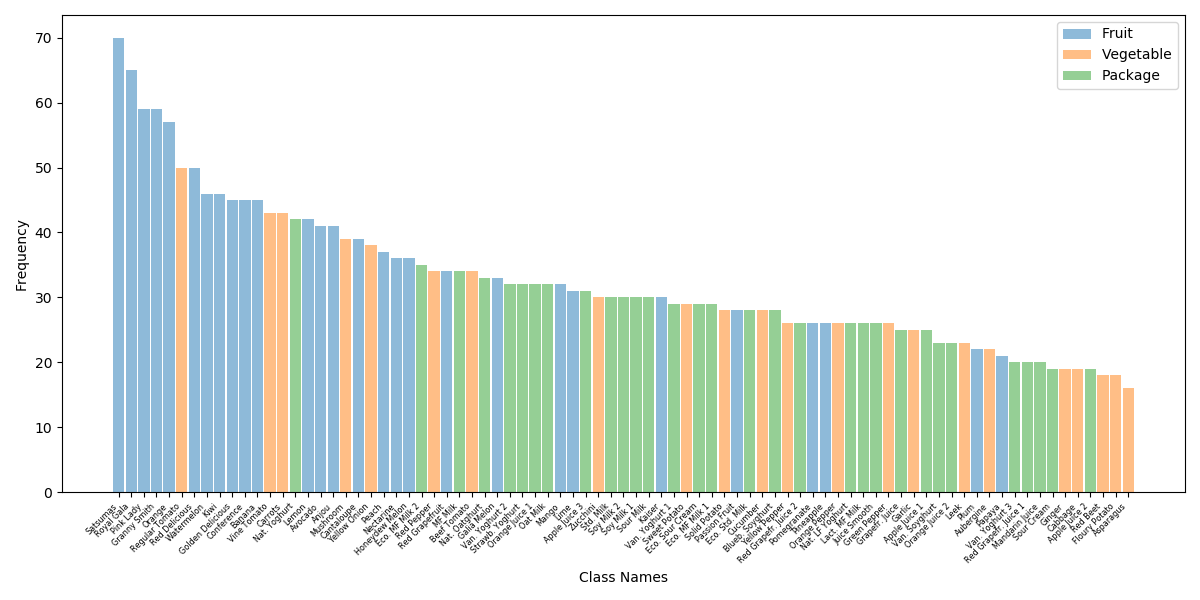
\includegraphics[width=\textwidth]{PaperB/appendix/figures/class_distributions_histogram/class_dist_train.png}
			%\vspace{-7mm}
			\caption{Histogram for the training split.}
			\label{fig:class_distribution_train}
		\end{subfigure} \\
		\begin{subfigure}[t]{0.82\linewidth}
			\centering
			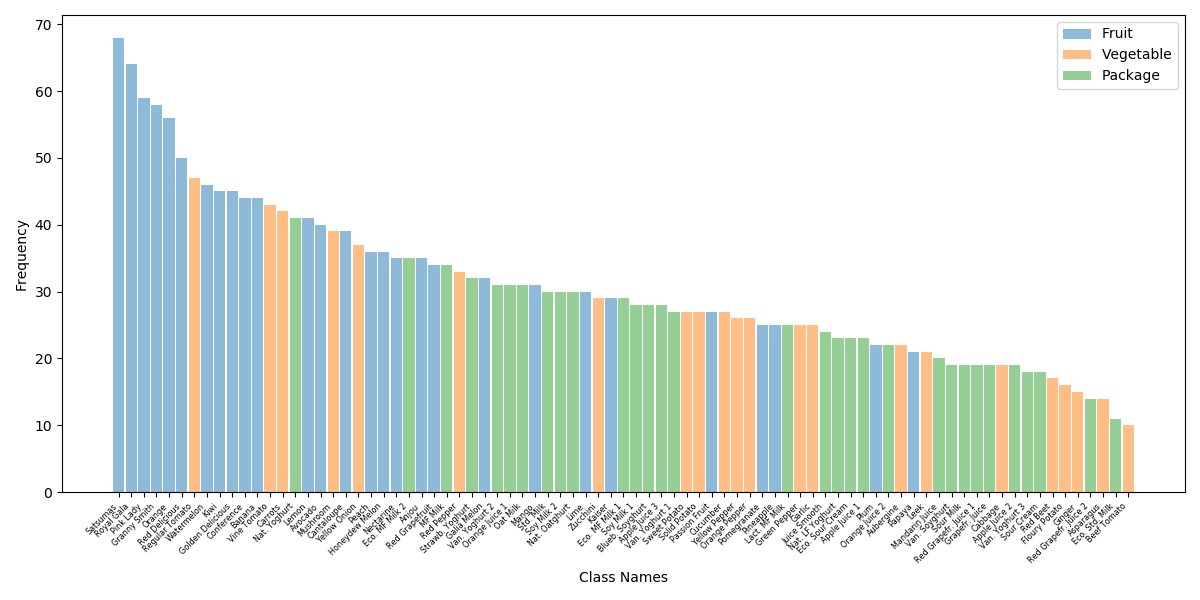
\includegraphics[width=\textwidth]{PaperB/appendix/figures/class_distributions_histogram/class_dist_test.png}
			%\vspace{-7mm}
			\caption{Histogram for the test split.}
			\label{fig:class_distribution_test}
		\end{subfigure} \\
		\begin{subfigure}[t]{0.82\linewidth}
			\centering
			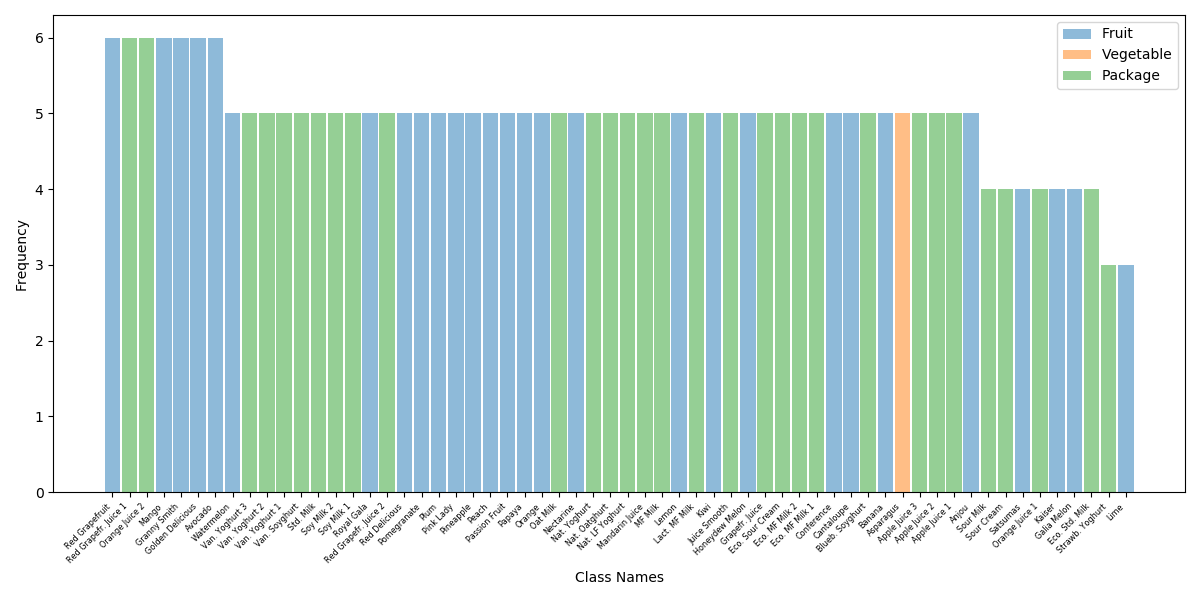
\includegraphics[width=\textwidth]{PaperB/appendix/figures/class_distributions_histogram/class_dist_val.png}
			%\vspace{-7mm}
			\caption{Histogram for the validation split.}
			\label{fig:class_distribution_val}
		\end{subfigure} 
	\end{minipage}
	\caption{Histograms of natural images for every class in the training (a), test (b), and validation (c) splits of the Grocery Store dataset. We also show with different colors on the bins if the class is either a Fruit, Vegetable, or Package item.}
	\label{paperB:fig:histograms}
\end{figure}


\clearpage
%\pagebreak




\clearpage

\begin{table}[!ht]
    %\begin{adjustwidth}{-1cm}{}
    \centering
    \caption{Examples of text descriptions and their corresponding class label and iconic image from the Grocery Store dataset. }
    \vspace{-2mm}
    \resizebox{\textwidth}{!}{
    \begin{tabular}{c c c}
         \toprule
         {\bf\footnotesize Class Label} & {\bf\footnotesize Iconic Image} & {\bf\footnotesize Text Description} \\
         \toprule
         \multicolumn{1}{p{1.5cm}}{\vspace{-17mm} {\footnotesize Golden Delicious Apple} } &
          \includegraphics[width=21mm, height=21mm]{PaperB/appendix/figures/iconic_images/Golden-Delicious-Apple_Clean.jpg}  & 
         \multicolumn{1}{p{12cm}}{\vspace{-15mm} {\footnotesize Golden Delicious has a white juicy pulp and a greenish yellow shell. The taste is mellow and sweet, making Golden Delicious suitable for desserts.} } \\
         
         \toprule
         \multicolumn{1}{p{1.5cm}}{\vspace{-17mm} {\footnotesize Red Delicious Apple} } & 
          \includegraphics[width=21mm, height=21mm]{PaperB/appendix/figures/iconic_images/Red-Delicious-Apple_Clean.jpg}  &  
         \multicolumn{1}{p{12cm}}{\vspace{-15mm} {\footnotesize Red Delicious is a dark red apple with relatively soft pulp and sweet taste.} } \\
         
         \toprule
         \multicolumn{1}{p{1.5cm}}{\vspace{-15mm} {\footnotesize Orange} } & 
          \includegraphics[width=21mm, height=21mm]{PaperB/appendix/figures/iconic_images/Orange_Clean.jpg}  & 
         \multicolumn{1}{p{12cm}}{\vspace{-17mm} {\footnotesize There are many different types of oranges that ripen and is sold during different parts of the year. The orange is a very important vitamin C source and the vitamins are best kept if the fruit is eaten naturally.} } \\
         
        \toprule
         \multicolumn{1}{p{1.5cm}}{\vspace{-15mm} {\footnotesize Yellow Bell Pepper} } & 
          \includegraphics[width=21mm, height=21mm]{PaperB/appendix/figures/iconic_images/Yellow-Pepper_Clean.jpg}  &  
         \multicolumn{1}{p{12cm}}{\vspace{-19mm} {\footnotesize The yellow pepper is much sweeter than the green. It also contains more vitamins and antioxidants than the green. Peppers are good to eat raw in salads and as garnish, but are also good to fry, stew or gratinate, for example with filling. Paprika also fits well in pots, gratins and pies.} } \\
         
         \toprule
         \multicolumn{1}{p{1.5cm}}{\vspace{-15mm} {\footnotesize Orange Bell Pepper} } & 
          \includegraphics[width=21mm, height=21mm]{PaperB/appendix/figures/iconic_images/Orange-Bell-Pepper_Iconic.jpg}  & 
         \multicolumn{1}{p{12cm}}{\vspace{-17mm} {\footnotesize The orange pepper is sweeter than the green. It also contains more vitamins and antioxidants than the green. Peppers are good to eat raw in salads and as garnish, but are also good to fry, stew or gratinate, for example with filling. Paprika also fits well in pots, gratins and pies.} } \\
         
         \toprule
         \multicolumn{1}{p{1.5cm}}{\vspace{-17mm} {\footnotesize Arla Medium Fat Milk} } &
         \includegraphics[width=21mm, height=21mm]{PaperB/appendix/figures/iconic_images/Arla-Milk-Medium-Fat_Clean.jpg} & 
         \multicolumn{1}{p{12cm}}{\vspace{-21mm} {\footnotesize Fresh skimmed milk made from Swedish milk from Arlagårdar. Skimmed milk has a delicious full-bodied milk flavor and is a popular choice for breakfast cereals, porridge or as a drink for the meal. Milk is a natural source of, for example, protein, calcium and vitamin B12. Protein contributes to muscle building and calcium is needed to maintain a normal bone structure. The brand Arla Ko guarantees that the product is made of 100\% Swedish milk.} } \\
         
         \toprule 
         \multicolumn{1}{p{1.5cm}}{\vspace{-18mm} {\footnotesize Arla Ecological Medium Fat Milk} } &
         \includegraphics[width=21mm, height=21mm]{PaperB/appendix/figures/iconic_images/Arla-Ecological-Medium-Fat-Milk_Iconic.jpg} & 
         \multicolumn{1}{p{12cm}}{\vspace{-22mm} {\footnotesize Fresh skimmed milk made from Swedish milk from organic Arlagårdar. Skimmed milk has a delicious full flavor and is a popular choice for breakfast cereals, porridge or as a drink for the meal. Milk is a natural source of, for example, protein, calcium and vitamin B12. Protein contributes to muscle building and calcium is needed to maintain a normal bone structure. The brand Arla Ko guarantees that the product is made of 100\% Swedish milk. The new brown carton has 24 percent lower climate impact compared to the previous white carton.} } \\
         
         
        \toprule
         \multicolumn{1}{p{1.5cm}}{\vspace{-17mm} {\footnotesize God Morgon Orange Juice} } &
          \includegraphics[width=21mm, height=21mm]{PaperB/appendix/figures/iconic_images/God-Morgon-Orange-Juice_Clean.jpg}  & 
         \multicolumn{1}{p{12cm}}{\vspace{-15mm} {\footnotesize God Morgon Orange is pressed by sun-dried, hand-picked oranges. The package contains juice from 2 kilograms of oranges!} } \\
         
         \toprule
         \multicolumn{1}{p{1.5cm}}{\vspace{-18mm} {\footnotesize Tropicana Golden Grapefruit Juice} } &
          \includegraphics[width=21mm, height=21mm]{PaperB/appendix/figures/iconic_images/Tropicana-Golden-Grapefruit_Clean.jpg}  & 
         \multicolumn{1}{p{12cm}}{\vspace{-17mm} {\footnotesize Tropicana Golden Grape is a ready to drink juice with pulp pressed on grapefruit. Not from concentrate. Mildly pasteurized.} } \\
         
        \toprule
    \end{tabular}
	}

    \label{paperB:tab:grocerystore_dataset_descriptions}
    %\end{adjustwidth}
\end{table}

\clearpage

\begin{table}[h]
\centering
\caption{ Classification accuracies on the test set for all models in percentage (\%) along with the best hyperparameter setting, i.e., the scaling weights $\lambda$ and text description length $T$, for each model. The column Accuracy corresponds to the fine-grained classification accuracy. The column Coarse Accuracy corresponds to the classifying a class within the correct parent class. Results are averaged using 10 different random seeds and we report both means and standard deviations. Abbreviations: AE, Autoencoder; VAE, Variational Autoencoder; SplitAE, Split Autoencoder; VCCA, Variational Canonical Correlation Analysis.
}
\vspace{-2mm}
\resizebox{\textwidth}{!}{%\scalebox{0.95}{
\begin{tabular}{l | c c c c | c | c c}
    \hline
    \Xhline{3\arrayrulewidth}
    Model & $\lambda_{x}$ & $\lambda_{i}$ & $\lambda_{w}$ & $\lambda_{y}$ & $T$ & Accuracy (\%) & Coarse Accuracy (\%) \\
    \Xhline{3\arrayrulewidth} 
    {\small DenseNet-scratch} & - & - & - & - & - & $67.33 \pm 1.35$ & $75.67 \pm 1.15$ \\ \hline

    {\small Softmax} & - & - & - & - &  - & $71.67 \pm 0.28$ & $83.34 \pm 0.32$ \\ \Xhline{2\arrayrulewidth}
    {\small AE$_{x}$+Softmax} & 1 & - & - & - &  - & $70.69 \pm 0.82$ & $82.42 \pm 0.58$ \\ \hline
    {\small VAE$_{x}$+Softmax} & 1 & - & - & - &  - & $69.20 \pm 0.46$ & $81.24 \pm 0.63$ \\ \Xhline{2\arrayrulewidth}
    
    {\small SplitAE$_{x y}$} & 1 & - & - & 1000 &  - & $70.34 \pm 0.56$ & $82.11 \pm 0.38$ \\ \hline
    {\small VCCA$_{x y}$} & 1 & - & - & 1000 &  - & $70.72 \pm 0.56$ & $82.12 \pm 0.61$ \\ \Xhline{2\arrayrulewidth}
    
    {\small SplitAE$_{x i}$+Softmax} & 1 & 1000 & - & - & - & $77.68 \pm 0.69$ & $87.09 \pm 0.53$ \\ \hline 
    {\small VCCA$_{x i}$+Softmax} & 1 & 1000 & - & - &  - & $77.02 \pm 0.51$ & $86.46 \pm 0.42$ \\ \hline 
    {\small VCCA-private$_{x i}$+Softmax} & 1 & 10 & - & - &  - & $73.04 \pm 0.56$ & $84.16 \pm 0.51$ \\    
    \Xhline{2\arrayrulewidth}
    
    {\small SplitAE$_{x i y}$} & 1 & 1000 & - & 1000 &  - & $77.43 \pm 0.80$ & $87.14 \pm 0.57$ \\ \hline    
    {\small VCCA$_{x i y}$} & 1 & 1000 & - & 1000 &  - & $77.22 \pm 0.55$ & $86.54 \pm 0.51$ \\ \hline
    {\small VCCA-private$_{x i y}$} & 1 & 10 & - & 1000 &  - & $74.04 \pm 0.83$ & $84.59 \pm 0.83$ \\      
    \Xhline{2\arrayrulewidth}
    
    {\small SplitAE$_{x w}$+Softmax} & 1 & - & 1000 & - &  40 & $76.27 \pm 0.66$ & $86.45 \pm 0.56$ \\ \hline 
    {\small VCCA$_{x w}$+Softmax} & 1 & - & 1000 & - &  75 & $75.37 \pm 0.46$ & $86.00 \pm 0.32$ \\ \hline 
    {\small VCCA-private$_{x w}$+Softmax} & 1 & - & 1000 & - &  75 & $75.11 \pm 0.81$ & $85.91 \pm 0.55$ \\
    \Xhline{2\arrayrulewidth} 
    
    {\small SplitAE$_{x w y}$} & 1 & - & 1000 & 10 &  75 & $75.78 \pm 0.84$ & $86.13 \pm 0.63$ \\ \hline
    {\small VCCA$_{x w y}$} & 1 & - & 1000 & 10 &  75 & $74.72 \pm 0.85$ & $85.59 \pm 0.78$ \\ \hline
    {\small VCCA-private$_{x w y}$} & 1 & - & 1000 & 1000 & 50 & $74.92 \pm 0.74$ & $85.59 \pm 0.67$ \\       
    \Xhline{2\arrayrulewidth} 
    
    {\small SplitAE$_{x i w}$+Softmax} & 1 & 1000 & 1000 & - &  24 & $77.79 \pm 0.48$ & $87.12 \pm 0.62$ \\
    {\small VCCA$_{x i w}$+Softmax} & 1 & 1000 & 1000 & - &  32 & $77.51 \pm \, 0.51$ & $86.69 \pm 0.41$ \\ \Xhline{2\arrayrulewidth}   
    
    {\small SplitAE$_{x i w y}$} & 1 & 1000 & 1000 & 1000 & 24 & $78.18 \pm 0.53$ & $87.26 \pm 0.46$ \\ 
    {\small VCCA$_{x i w y}$} & 1 & 1000 & 1000 & 1000 &  91 & $77.78 \pm 0.45$ & $86.88 \pm 0.47$ \\ 
    \Xhline{3\arrayrulewidth}
\end{tabular}
}
\vspace{-2mm}
\label{paperB:tab:classification_results_on_test_set_with_hyperparameters}
\end{table}

%\clearpage


	
	%\newpage
	
	\section{Supplemental Experimental Procedures}
	
\subsection{Details on Experimental Setup}
\label{paperB:app:details_on_experimental_setup}

In this section, we provide the full details on the experimental setups.

\vspace{-3mm}
\paragraph{Training DenseNet169 from Scratch} We train a DenseNet169 on the dataset from scratch as a baseline. We train the network using stochastic gradient descent for 300 epochs and follow the learning rate schedule of Huang \etal~\citeB{B:huang2017densely}, i.e., using an initial learning rate of 0.1 and dividing it by 10 after 150 and 225 epochs. We use a weight decay of $10^{-4}$ and Nesterov momentum of 0.9 without dampening. We denote this network as DenseNet-scratch in the experiments.

\vspace{-3mm}
\paragraph{Training the Softmax Classifier} We use a Softmax classifier trained on off-the-shelf features as another baseline. We use a DenseNet169~\citeB{B:huang2017densely} pre-trained on ImageNet 1K as the feature extractor, where we extract 1664-dimensional from the average pooling layer before the classification layer in the architecture. The Softmax classifier is trained for 100 epochs with batch size 64 to minimize the cross-entropy loss. We use the Adam optimizer~\citeB{B:kingma2015adam} with initial learning rate $10^{-4}$ and hyperparameters $\beta_1 = 0.5$ and $\beta_2 = 0.999$. Note that we used no regularization when training the Softmax classifier. We denote this classifier as Softmax in the experiments. This training setup is also used when training the Softmax classifiers for SplitAE, VCCA, and VCCA-private. 

\vspace{-3mm}
\paragraph{Architectures for Single-View Autoencoders} We use a vanilla autoencoder and a VAE as baselines that learn latent representations of the natural image features only. These models are denoted as AE$_{x}$ and VAE$_{x}$ respectively in the experiments. Their latent representations have dimension $d_{z} = 200$ throughout all experiments. The encoder and decoder networks consist of one hidden layer of $512$ hidden units with Leaky ReLU activation. The decoder aims to reconstruct the natural image features and we use the sum-of-squares as the reconstruction loss during training. For the VAE, we use the mean outputs $\mu_{z}(x)$ from the encoder as the latent representations of the image features to train a Softmax classifier, which we denote as VAE$_{x}$+Softmax.

\vspace{-3mm}
\paragraph{Architectures for SplitAE and VCCA} We use the same encoder and decoder architecture for the natural image features as in the single-view autoencoders for all SplitAE, VCCA, and VCCA-private models, i.e., one hidden layer of $512$ hidden units with Leaky ReLU activation. We set the latent dimension to $d_{z} = 200$ in all experiments. The class label decoders use the same architecture as the image feature decoder and predict the class label by optimizing the cross-entropy loss. The iconic image decoders use the generator architecture of the DCGAN~\citeB{B:radford2015unsupervised}. This decoder reconstructs the iconic images $i \in \R^{64 \times 64 \times 3}$ by minimizing the sum of squares loss. The text descriptions are assumed to be a sequence of words $w = (w_1, \dots, w_T)$, where $T$ is the length of the description. We create a vocabulary $V \in \mathbb{R}^{658}$ of the total number of unique words from all text descriptions in the dataset. The text description decoder is an LSTM~\citeB{B:hochreiter1997long} followed by a linear layer that predicts the next word in the description. More specifically, at time step $t$, the decoder yields a multinomial probability distribution $p_{{\theta_{w}}}(w_t | w_{t-1}, z)$ defined over $w_t \in V$. The LSTM is trained using teacher forcing, meaning that we use the previous ground truth word as input at every time step during the training phase. We project each word into an embedding space of dimensionality $d_{emb} = 200$ by using a lookup table before the word is input to the LSTM. The hidden state $h$ and memory state $c$ of the LSTM is initialized with a linear projection of the latent representation $z$ to provide the LSTM with some context about the natural image. We use the same dimension for $h$ and $c$ as for $z$, i.e., $d_{z} = d_{h} = d_{c} = 200$. We minimize the cross-entropy loss at every time step by comparing the predicted word with the true word in the description. We apply dropout~\citeB{B:srivastava2014dropout} with a keep rate of 0.5 on the output hidden state $h_t$ before we input it through the linear layer that predicts the word at time step $t$. 

\vspace{-3mm}
\paragraph{Architectures for VCCA-private} In the VCCA-private models, the decoders has the same architectures as the VCCA models. The encoder for the shared latent variable $z$ is also the same as the encoder for the previous described models. The encoder for the private latent variable $u_{x}$ uses an identical architecture as encoder for $z$. We use a convolutional encoder for the iconic image private latent variable, which is a reversed DCGAN generator outputting the mean $\mu_{u_{i}}(i)$ and variance ${\sigma}_{u_{i}}^2(i)$. The text description encoder is an LSTM with the same architectural details as the LSTM decoder. We obtain an embedding for the description by averaging all of the hidden states $h_t$ generated from the LSTM, i.e., $\frac{1}{T} \sum_{t=1}^{T} h_t$, and input it to a linear layer outputting the mean $\mu_{u_{w}}(w)$ and the variance ${\sigma}_{u_{w}}^2(w)$ for the private latent variable for the text description. We use the same latent dimensions for the shared and private latent variables, i.e., $d_{z} = d_{u_{x}} = d_{u_{i}} = d_{u_{w}} = 200$. 

\vspace{-3mm}
\paragraph{Training the Single- and Multi-View Autoencoders} The single- and multi-view autoencoding models are trained for 200 epochs with batch size 64 and aims to minimize either their reconstruction losses or their corresponding ELBOs. We use the Adam optimizer with initial learning rate $10^{-4}$ and hyperparameters $\beta_1 = 0.9$ and $\beta_2 = 0.999$ in all experiments. The mean outputs $\mu_{z}(x)$ from the encoder are used as the latent representations of the image features to train a Softmax classifier. For the class label decoder, we use $K=1$ posterior samples for predicting the class label during training, while we set $K=5$ in the validation and test stages. 

\vspace{-3mm}
\paragraph{Grid Search} We run a hyperparameter search for the scaling weights $\lambda$ for the reconstruction losses of the views using a grid search with grid points $\{0.1, 1, 10, 100, 1000\}$. The grid search is performed for all VCCA and VCCA-private models. The weight for the natural image feature loss $\lambda_{x}$ is used as a reference by setting it to $\lambda_{x}=1$ throughout all experiments. This means that we only vary the scaling weights $\lambda_{i}$, $\lambda_{w}$, and $\lambda_{y}$. We run the grid searches using three different random seeds and average the resulting validation accuracies to select the best hyperparameter setting. Table \ref{paperB:tab:classification_results_on_test_set_with_hyperparameters}
shows the best hyperparameter settings for the VCCA and VCCA-private models with their test %validation 
accuracies. Note that we use the same scaling weights for SplitAE as the ones we found for its corresponding VCCA model. To summarize the grid search results, it is always beneficial to use scaling weights $\lambda > 1$ for the models to enhance the classification accuracy. This will make the models add some semantically meaningful information to the latent space from the additional views, which makes the models more suitable for downstream tasks such as classification. 

	
	\subsection*{Posterior Collapse in VCCA-private}
\label{paperB:app:posterior_collapse_in_vcca_private}

We noticed in Table 1 that VCCA-private achieves similar classification performance as standard VCCA when utilizing the text description $w$ and even worse results when utilizing the iconic image $i$. The private latent variables cannot capture any view-specific variations when each class uses the same iconic image and text description for every natural image. 
A consequence of this is that the iconic image and text description can be identified by only using the shared latent variable $z$ in the decoding phase. The private latent variables are thus not necessary for determining which iconic image or text description to generate, the generated view will be the same anyway for every natural image of a specific class. The model then finds out that the ELBO can be maximized by letting the approximate posteriors be equal to their prior distributions, which minimize the KL divergences of the private latent variables. This phenomenon is referred to as \textit{posterior collapse}~\citeB{B:bowman2015generating}. 

In Figure \ref{fig:kl_divergence_vcca_private} and \ref{fig:kl_divergence_vcca_private_with_iconic_image}, we illustrate that the approximate posterior deduces to its prior distribution -- a zero-mean Gaussian with unit variance -- during training. Figure \ref{fig:kl_divergence_vcca_private}(a) and \ref{fig:kl_divergence_vcca_private}(b) shows the KL divergences over epochs for VCCA-private$_{x w}$ and VCCA-private$_{x w y}$ respectively. The number of words $T=24$ is the same for both models and we train the models for 500 epochs to emphasize that $\KL(q_{\phi_{w}}(u_{w} |w)\,||\,p(u_{w}))$ goes towards zero. We believe that this is due to that there are no variations in the text descriptions within one class (see subsection Investigations of the Learned Representations in Results). We perform a similar experiment with VCCA-private$_{x i}$ and VCCA-private$_{x i y}$ and plot their KL divergences in Figure \ref{fig:kl_divergence_vcca_private_with_iconic_image}. The KL divergence $\KL(q_{\phi_{i}}(u_{i} |w)\,||\,p(u_{i}))$ decreases to zero faster for these models than when we use the text description. We also observe that the KL divergence $\KL(q_{\phi_{x}}(u_{x} |x)\,||\,p(u_{x}))$ decreases to zero as well for both models. Why the KL divergence for the private latent variables decreases faster in the models with the iconic image $i$ is mainly because their likelihood weight $\lambda_{i}$ is smaller than $\lambda_{w}$. We noticed that the KL divergences of the private latent variables decreases slower towards zero when $\lambda_{i}$ is increased, probably because the model foremost focuses on minimizing the reconstruction loss. 


	
	
\subsection{Investigating Latent Representations in VCCA-private\texorpdfstring{$_{x i}$}{TEXT}}
\label{paperB:app:investigating_latent_representations_in_vcca_private_xi}

Figure \ref{fig:2d_visualizations_pca_vcca_private_xi} shows the shared and private latent spaces of VCCA-private$_{x i}$, as well as the latent space of the standard VCCA$_{x i}$ for comparison. Note that the shared latent spaces in Figure \ref{fig:2d_visualizations_pca_vcca_private_xi}(a) and \ref{fig:2d_visualizations_pca_vcca_private_xi}(b) have different structures mainly due to the different settings of their likelihood weight $\lambda_{i}$, which is $\lambda_{i} = 1000$ for VCCA$_{x i}$ and $\lambda_{i} = 10$ for VCCA-private$_{x i}$. We observe in Figure \ref{fig:2d_visualizations_pca_vcca_private_xi}(c) that the natural images are structured based on their similarities in background and camera setup. Across the upper right and the lower left parts of the cluster, we find images of grocery items closely packed together in bins. The middle and upper left part includes images with the hand of the photographer and grey backgrounds, e.g., the floor and shelves in the grocery store. Note that this private latent space is rather densely packed mainly because the KL divergence $\KL(q_{\phi_{x}}(u_{x} |x)\,||\,p(u_{x}))$ is steadily decreasing towards zero (see Figure \ref{fig:kl_divergence_vcca_private_with_iconic_image}(a)). This means that the approximate posterior $q_{\phi_{x}}(u_{x} |x)$ is collapsing to its prior distribution, which is why the mean values $\mu_{u_{x}}$ are close to the origin of the space. The mean values $\mu_{u_{i}}$ for the private latent variable $u_{i}$ are shown in Figure \ref{fig:2d_visualizations_pca_vcca_private_xi}(d) using the iconic image. Note that every iconic image $i$ is projected at the same location in the latent space. We observe that similar iconic images are projected close to each other. For instance, an orange, grapefruit and yellow bell pepper have been projected in the upper part, packaged items are in the center parts and the left region we find round objects with a dark red color. To the far right, we see a green and a red apple that has been pushed far away from the similar iconic images on the left. If we look closer into these iconic images, we observe that the apples on the right have a higher stalk on top of the apple than the apples on the left side has, which could be the reason why the model has separated them in the latent space. Another interesting observation is that iconic images with multiple items, e.g., tomatoes, kiwis and satsumas, have been projected into the lower region of the space. We conclude that similar iconic images, based on color and their appearance in the image, are grouped closely in the private latent space.  


\begin{figure}[th!]
	\centering
	\begin{minipage}{\textwidth}
		\centering
		\begin{subfigure}[t]{0.48\textwidth}
			\centering
			\includegraphics[width=\textwidth]{PaperB/appendix/figures/vcca_private_xi/pca_vcca_xi.png}
			\caption{$\mu_{z}$ from VCCA$_{x i}$}
			\label{fig:pca_vcca_xi_z}
		\end{subfigure}~
		\begin{subfigure}[t]{0.48\textwidth}
			\centering
			\includegraphics[width=\textwidth]{PaperB/appendix/figures/vcca_private_xi/pca_z_vcca_private_xi_seed1.png}
			\caption{$\mu_{z}$ from VCCA-private$_{x i}$}
			\label{fig:pca_vcca_private_xi_z}
		\end{subfigure}
		%\subfigure[$\mu_{z}$ from VCCA$_{x i}$ ]{\label{fig:pca_vcca_xi_z}\includegraphics[width=0.45\textwidth]{PaperB/appendix/figures/vcca_private_xi/pca_vcca_xi.png}}~
		%\subfigure[$\mu_{z}$ from VCCA-private$_{x i}$]{\label{fig:pca_vcca_private_xi_z}\includegraphics[width=0.45\textwidth]{PaperB/appendix/figures/vcca_private_xi/pca_z_vcca_private_xi_seed1.png}}\\ 
	\end{minipage}
	\begin{minipage}{0.8\textwidth}
		\centering
		\begin{subfigure}[t]{0.6\textwidth}
			\centering
			\includegraphics[width=\textwidth]{PaperB/appendix/figures/vcca_private_xi/vcca_private_xi_ux_space.pdf}
			\caption{$\mu_{u_{x}}$ from VCCA-private$_{x i}$}
			\label{fig:pca_vcca_private_xi_ux}
		\end{subfigure} \\
		\begin{subfigure}[t]{0.75\textwidth}
			\centering
			\includegraphics[width=\textwidth]{PaperB/appendix/figures/vcca_private_xi/vcca_private_xi_ui_space.pdf}
			\caption{$\mu_{u_{i}}$ from VCCA-private$_{x i}$}
			\label{fig:pca_vcca_private_xi_ui}
		\end{subfigure}
	\end{minipage}
	\caption{Visualizations of the latent representations $\mu_{z}(x)$ from VCCA$_{x i}$ and VCCA-private$_{x i}$ on the first row followed by $\mu_{u_{x}}(x)$ and $\mu_{u_{i}}(i)$ for VCCA-private$_{x i}$. Abbreviations: VCCA, Variational Canonical Correlation Analysis.}
	\label{fig:2d_visualizations_pca_vcca_private_xi}
\end{figure}

\clearpage
	
	
\subsection{Derivation of the ELBO for VCCA}
\label{paperB:app:derivation_of_elbo_for_vcca}

Let $x_{1:M}$ denote the all observed data, i.e., $x_{1:M} = x_1, \dots, x_M$, for $M$ different views. We derive the ELBO for VCCA by introducing the approximate posterior $q_{\phi}(z | x_m)$, where $x_m$ is the only view that we use to infer the latent variable $z$. We now derive the ELBO from the marginal log-likelihood $ \log p_{{\theta}}(x_{1:M})$ as 
\begin{align*}
    \begin{split}
        \log p_{{\theta}}(x_{1:M}) = & \log p_{{\theta}}(x_{1:M}) \int q_{\phi}(z | x_m) \, dz \\
        = & \int q_{\phi}(z | x_m) \log p_{{\theta}}(x_{1:M}) \, dz \\
        = & \int q_{\phi}(z | x_m) \log \frac{p_{{\theta}}(x_{1:M}, z)}{p_{{\theta}}(z | x_{1:M})}  \, dz \\
        = & \int q_{\phi}(z | x_m) \log \frac{p_{{\theta}}(x_{1:M}, z)}{p_{{\theta}}(z | x_{1:M})} \frac{q_{\phi}(z | x_m)}{q_{\phi}(z | x_m)}  \, dz \\
        = & \int q_{\phi}(z | x_m) \left( \log \frac{q_{\phi}(z | x_m)}{p_{{\theta}}(z | x_{1:M})} + \log \frac{p_{{\theta}}(x_{1:M}, z)}{q_{\phi}(z | x_m)} \right) dz \\
        = & \, \KL(q_{\phi}(z | x_m) \,||\, p_{{\theta}}(z | x_{1:M})) + \E_{q_{\phi}(z | x_m)}\left[ \log \frac{p_{{\theta}}(x_{1:M}, z)}{q_{\phi}(z | x_m)} \right] \\
        \geq & \, \E_{q_{\phi}(z | x_m)}\left[ \log \frac{p_{{\theta}}(x_{1:M}, z)}{q_{\phi}(z | x_m)} \right] = \mathcal{L}(x_{1:M}; \theta, \phi)
    \end{split}
\end{align*}
We use the factorization property of the joint distribution $p_{\theta}(x_{1:M})$ to further derive the ELBO $\mathcal{L}(x_{1:M}; \theta, \phi)$:
\begin{align*}
    \begin{split}
        \mathcal{L}(\theta, \phi; x_{1:M}) = & \E_{q_{\phi}(z | x_m)}\left[ \log \frac{p_{{\theta}_1}(x_1 |  z) \cdots p_{{\theta}_M}(x_M |  z) p(z)}{q_{\phi}(z | x_m)} \right] \\
        = & \E_{q_{\phi}(z | x_m)}\left[ \log p_{{\theta}_1}(x_1 |  z) + ... + \log p_{{\theta}_M}(x_M |  z) + \log \frac{p(z)}{q_{\phi}(z | x_m)} \right] \\
        = & \E_{q_{\phi}(z | x_m)}\left[ \log p_{{\theta}_1}(x_1 |  z) \right] + ... + \E_{q_{\phi}(z | x_m)}\left[ \log p_{{\theta}_M}(x_M |  z) \right] \\ 
        & -\KL(q_{\phi}(z | x_m) \,||\, p(z))
    \end{split}
\end{align*}
It may be necessary to balance the terms in the ELBO with some constant for every term, especially when the dimensions and magnitudes differ between the modalities. Thus, we introduce the likelihood weights $\lambda_1, ..., \lambda_M$, such that the ELBO will be written as 
\begin{align*}
    \begin{split}
        \mathcal{L}(\theta, \phi; x_{1:M}) = & \lambda_1 \E_{q_{\phi}(z | x_m)}\left[ \log p_{{\theta}_1}(x_1 |  z) \right] + ... + \lambda_M \E_{q_{\phi}(z | x_m)}\left[ \log p_{{\theta}_M}(x_M |  z) \right] \\
        & - \KL(q_{\phi}(z | x_m) \,||\, p(z)) 
    \end{split}
\end{align*}
The likelihood weights $\lambda_1, ..., \lambda_M$ that are optimal for the task at hand can be found with some hyperparameter search.
\end{appendices}
%\appendix
%\renewcommand{\thesection}{\Roman{section}}
%
%%%%%%%%% BODY TEXT

\section*{Appendix}
This supplementary material is structured as follows: 
\begin{itemize}[noitemsep]
	\item Appendix \ref{paperC:app:rs_mcts_algorithm}: Pseudocode of MCTS in Algorithm \ref{alg:replay_scheduling_mcts} to provide more details about our method. 
	\item Appendix \ref{paperC:app:experimental_settings}: Full details of the experimental settings.
	%\item Appendix \ref{paperC:app:heuristic_scheduling_baseline} describes the Heuristic scheduling baseline.
	\item Appendix \ref{paperC:app:additional_experimental_results} shows additional experimental results. 
	%\item Appendix \ref{paperC:app:additional_figures} includes additional figures. 
	%\item Our code is provided in the zip-file {\footnotesize \texttt{code\_replay\_scheduling\_mcts\_icml22.zip}} as part of the supplementary material and will be made publicly available upon acceptance. 
\end{itemize}


%------------------------------------------------------------------------


\section[Replay Scheduling MCTS Algorithm]{Replay Scheduling Monte Carlo Tree Search Algorithm}\label{paperC:app:rs_mcts_algorithm}

%%% MCTS ALGORITHMS


In this section, we provide more details on the methodology for replay scheduling with MCTS. Algorithm \ref{paperC:alg:action_space_discretization} outlines the steps for how we discretized the action space of task proportions to enable searching for replay schedules (Section \ref{paperC:sec:replay_scheduling_in_continual_learning}). Furthermore, we provide pseudo-code in Algorithm \ref{alg:replay_scheduling_mcts} outlining the steps for our method Replay Scheduling Monte Carlo tree search (RS-MCTS) described Section \ref{paperC:sec:mcts_for_replay_scheduling}. %in the main paper (Section \ref{paperC:sec:mcts_for_replay_scheduling}). 

In Algorithm \ref{alg:replay_scheduling_mcts}, the MCTS procedure selects actions over which task proportions to fill the replay memory with at every task, where the selected task proportions are stored in the replay schedule $S$. The schedule is then passed to 
the function \textsc{EvaluateReplaySchedule$(\cdot)$} 
where the continual learning part executes the training with replay memories filled according to the schedule. The reward for the schedule $S$ is the average validation accuracy over all tasks after learning task $T$, i.e., ACC, which is backpropagated through the tree to update the statistics of the selected nodes. The schedule $S_{best}$ yielding the best ACC score is returned to be used for evaluation on the held-out test sets. The function $\textsc{GetReplayMemory}(\cdot)$ is the policy for retrieving the replay memory $\gM$ from the historical data given the task proportion $\va$. The number of samples per task determined by the task proportions are rounded up or down accordingly to fill $\gM$ with $M$ replay samples in total. 
The function $\textsc{GetTaskProportion}(\cdot)$ simply returns the task proportion that is related to given node.



\begin{algorithm}[h!]
	\small
	\caption{Discretization of action space with task proportions}
	\label{paperC:alg:action_space_discretization}
	\begin{algorithmic}[1]
		\Require Number of tasks $T$
		\State $\gT = ()$ \Comment{Initialize sequence for storing actions}
		\For{$i = 1, \dots, T-1$}
		\State $\gP_i = \{\}$ \Comment{Set for storing task proportions at $i$}
		\State $\gB = \texttt{combinations}([1:i], i)$ \Comment{Get bin vectors of size $i$ with bins $1, ..., i$}
		\State $\bar{\gB} = \texttt{unique}(\texttt{sort}(\gB))$ \Comment{Only keep unique bin vectors}
		\For{$\vb_i \in \hat{\gB}$}
		\State $\va_i = \texttt{bincount}(\vb_i) / i$ \Comment{Calculate task proportion}
		\State $\gP_i = \gP_i \cup \{ \va_i \}$ \Comment{Add task proportion to set}
		\EndFor
		\State $\gT[i] = \gP_i$ \Comment{Add set of task proportions to action sequence}
		\EndFor
		\State \Return $\gT$ \Comment{Return action sequence as discrete action space}
	\end{algorithmic}
\end{algorithm}



\begin{algorithm}[h!]
\caption{Replay Scheduling Monte Carlo tree search}
\label{alg:replay_scheduling_mcts}
\algrenewcommand\alglinenumber[1]{\tiny #1:}
\scriptsize
\begin{algorithmic}[1]
\Require Tree nodes $v_{1:T}$, Datasets $\gD_{1:T}$, Learning rate $\eta$
\Require Replay memory size $M$ %, Historical data sample size $H$
%\State Initialize historical data $\gH$ using $\gD_{1:T}$
%\State Initialize model $\vtheta_0$
\State $\textnormal{ACC}_{best} \leftarrow 0$, $S_{best} \leftarrow ()$
%\State $\vtheta_1 \leftarrow \textsc{TrainModel}(\gD_1, \vtheta_0)$
\While{within computational budget}
    \State $S \leftarrow ()$
    \State $v_{t}, S \leftarrow \textsc{TreePolicy}(v_1, S)$%\State $v_{t}, \vtheta_t \leftarrow \textsc{TreePolicy}(v_1, \vtheta_1, \gD_{1:T}, \gH, M)$
    \State $v_{T}, S \leftarrow \textsc{DefaultPolicy}(v_{t}, S)$%\State $v_{t}, \vtheta_T, \textnormal{acc} \leftarrow \textsc{DefaultPolicy}(v_{t}, \vtheta_t, \gD_{1:T}, \gH, M)$
    \State ACC $\leftarrow \textsc{EvaluateReplaySchedule}(\gD_{1:T}, S, M)$
    \State $\textsc{Backpropagate}(v_{t}, \textnormal{ACC})$
    \If{$\textnormal{ACC} > \textnormal{ACC}_{best}$}
        %\State $v_T^{best} \leftarrow v_T$
        %\State $\vtheta_T^{best} \leftarrow \vtheta_{T}$
        \State $\textnormal{ACC}_{best} \leftarrow \textnormal{ACC}$
        \State $S_{best} \leftarrow S$
    \EndIf
\EndWhile
\State \Return $\textnormal{ACC}_{best}, S_{best}$

\Statex 
\vspace{-3pt}
\Function{TreePolicy}{$v_t, S$}
\While{$v_t$ is non-terminal}  
\If{$v_t$ not fully expanded}
    \State \Return $\textsc{Expansion}(v_t, S)$
\Else
    \State $v_{t} \leftarrow \textsc{BestChild}(v_t)$
    %\State $\va_{t} \leftarrow \textsc{GetTaskProportion}(v_t)$
    \State $S$.append$(\va_{t})$, where $\va_{t} \leftarrow \textsc{GetTaskProportion}(v_t)$
\EndIf
\EndWhile
\State \Return $v_t, S$
\EndFunction

\Statex

\Function{Expansion}{$v_t, S$}
\State Sample $v_{t+1}$ uniformly among unvisited children of $v_t$
%\State $\gM \stackrel{M}{\sim} \gH$ using memory combination in $v_{t+1}$
%\State $\vtheta_{t+1} \leftarrow \textsc{TrainModel}(\gD_{t+1} \cup \gM, \vtheta_{t})$
%\State $\va_{t+1} \leftarrow \textsc{GetTaskProportion}(v_{t+1})$
\State $S$.append$(\va_{t+1})$, where $\va_{t+1} \leftarrow \textsc{GetTaskProportion}(v_{t+1})$
\State Add new child $v_{t+1}$ to node $v_{t}$%\State Add new child $v_{t+1}$ with model $\vtheta_{t+1}$ to node $v_{t}$
\State \Return $v_{t+1}, S$
\EndFunction

\Statex 

\Function{BestChild}{$v_t$}
    \State $v_{t+1} =   \argmax\limits_{v_{t+1} \in \text{ children of } v} \text{max}(Q(v_{t+1})) + C \sqrt{\frac{2 \log(N(v_{t}))}{N(v_{t+1})}}$
    %\State Get model $\vtheta_{t+1}$ from node $v_{t+1}$
    \State \Return $v_{t+1}$
\EndFunction

\Statex 

\Function{DefaultPolicy}{$v_t, S$}
\While{$v_t$ is non-terminal}  
    \State Sample $v_{t+1}$ uniformly among children of $v_t$
    %\State $\va_{t+1} \leftarrow \textsc{GetTaskProportion}(v_{t+1})$
    \State $S$.append$(\va_{t+1})$, where $\va_{t+1} \leftarrow \textsc{GetTaskProportion}(v_{t+1})$
    %\State $\gM \stackrel{M}{\sim} \gH$ using memory combination in $v_{t+1}$
    %\State $\vtheta_{t+1} \leftarrow \textsc{TrainModel}(\gD_{t+1} \cup \gM, \vtheta_{t})$
    \State Update $v_{t} \leftarrow v_{t+1}$ %, $\vtheta_{t} \leftarrow \vtheta_{t+1}$
\EndWhile
%\State $\textnormal{acc} \leftarrow \textsc{TestModel}(\gD_{1:T}, \vtheta_{t})$
\State \Return $v_t, S$
\EndFunction

\Statex

\Function{EvaluateReplaySchedule}{$\gD_{1:T}, S, M$}
\State Initialize neural network $f_{\vtheta}$
%\State $\gH \leftarrow \{\}$
\For{$t = 1, \dots, T$}  
    \State $\va \leftarrow S[t-1]$
    \State $\gM \leftarrow \textsc{GetReplayMemory}(M, \va)$
    \For{$ \gB \sim \gD_t^{(train)}$}  
        \State $\vtheta \leftarrow SGD(\gB \cup \gM, \vtheta, \eta)$ 
        %\State $Q(v_t) \leftarrow R$
        %\State $v_t \leftarrow$ parent of $v_t$
    \EndFor
    %\State $\gH \leftarrow \textsc{UpdateHistoricalData}(\gD_t^{(train)}, H)$
\EndFor
\State $A_{1:T}^{(val)} \leftarrow \textsc{EvaluateAccuracy}(f_{\vtheta}, \gD_{1:T}^{(val)})$
\State $\textnormal{ACC} \leftarrow \frac{1}{T} \sum_{i=1}^{T} A_{T,i}^{(val)}$
\State \Return ACC
\EndFunction

\Statex

\Function{Backpropagate}{$v_t, R$}
\While{$v_t$ is not root}  
    \State $N(v_t) \leftarrow N(v_t)+1$
    \State $Q(v_t) \leftarrow R$
    \State $v_t \leftarrow$ parent of $v_t$
\EndWhile
\EndFunction
\end{algorithmic}
\end{algorithm}







\clearpage



\section{Experimental Settings}\label{app:experimental_settings}

In this section, we describe the full details of the experimental settings used in this paper. 

\vspace{-2mm}
\paragraph{Datasets.}
We conduct experiments on six datasets commonly used in the continual learning literature. Split MNIST~\citeC{C:zenke2017continual} is a variant of the MNIST~\citeC{C:lecun1998gradient} dataset where the classes have been divided into 5 tasks incoming in the order 0/1, 2/3, 4/5, 6/7, and 8/9. Split Fashion-MNIST~\citeC{C:xiao2017fashion} is of similar size to MNIST and consists of grayscale images of different clothes, where the classes have been divided into the 5 tasks T-shirt/Trouser, Pullover/Dress, Coat/Sandals, Shirt/Sneaker, and Bag/Ankle boots. Similar to MNIST, Split notMNIST~\citeC{C:bulatov2011notMNIST} consists of 10 classes of the letters A-J with various fonts, where the classes are divided into the 5 tasks A/B, C/D, E/F, G/H, and I/J. We use training/test split provided by \citetC{C:ebrahimi2020adversarial} for Split notMNIST. Permuted MNIST~\citeC{C:goodfellow2013empirical} dataset consists of applying a unique random permutation of the pixels of the images in original MNIST to create each task, except for the first task that is to learn the original MNIST dataset. We reduce the original MNIST dataset to 10k samples and create 9 unique random permutations to get a 10-task version of Permuted MNIST. In Split CIFAR-100~\citeC{C:krizhevsky2009learning}, the 100 classes are divided into 20 tasks with 5 classes for each task~\citeC{C:lopez2017gradient, rebuffi2017icarl}. Similarly, Split miniImagenet~\citeC{C:vinyals2016matching} consists of 100 classes randomly chosen from the original Imagenet dataset where the 100 classes are divided into 20 tasks with 5 classes per task.

\vspace{-2mm}
\paragraph{Network Architectures.} We use a 2-layer MLP with 256 hidden units and ReLU activation for Split MNIST, Split FashionMNIST, Split notMNIST, and Permuted MNIST. We use a multi-head output layer for each dataset except Permuted MNIST where the network uses single-head output layer. For Split CIFAR-100, we use a multi-head CNN architecture built according to the CNN in \citeC{C:adel2019continual, C:schwarz2018progress, C:vinyals2016matching}, which consists of four 3x3 convolutional blocks, i.e. convolutional layer followed by batch normalization~\citeC{C:ioffe2015batch}, with 64 filters, ReLU activations, and 2x2 Max-pooling. For Split mniImagenet, we use the reduced ResNet-18 from \citeC{C:lopez2017gradient} with multi-head output layer. 

\vspace{-2mm}
\paragraph{Hyperparameters.} We train all networks with the Adam optimizer~\citeC{C:kingma2014adam} with learning rate $\eta = 0.001$ and hyperparameters $\beta_1 = 0.9$ and $\beta_2 = 0.999$. Note that the learning rate for Adam is not reset before training on a new task. Next, we give details on number of training epochs and batch sizes specific for each dataset:
\begin{itemize}[topsep=1pt]
    \item Split MNIST: 10 epochs/task, batch size 128.
    \item Split FashionMNIST: 30 epochs/task, batch size 128.
    \item Split notMNIST: 50 epochs/task, batch size 128.
    \item Permuted MNIST: 20 epochs/task, batch size 128.
    \item Split CIFAR-100: 25 epochs/task, batch size 256.
    \item Split miniImagenet: 1 epoch/task (task 1 trained for 5 epochs as warm up), batch size 32.
\end{itemize}

\vspace{-2mm}
\paragraph{Monte Carlo Tree Search.} We run RS-MCTS for 100 iterations in all experiments. The replay schedules used in the reported results on the held-out test sets are from the replay schedule that gave the highest reward on the validation sets. The exploration constant for UCT in Equation \ref{eq:uct} is set to $C=0.1$ in all experiments~\citeC{C:chaudhry2018feature}.

\vspace{-2mm}
\paragraph{Computational Cost.} All experiments were performed on one NVIDIA GeForce RTW 2080Ti. The wall clock time for ETS on Split MNIST was around 1.5 minutes, and RS-MCTS and BFS takes 40 seconds on average to run one iteration, where BFS runs 1050 iterations in total for Split MNIST. 


\vspace{-2mm}
\paragraph{Implementations.} We adapted the implementation released by Borsos \etal~\citeC{C:borsos2020coresets} for the memory selection strategies Uniform sampling, $k$-means clustering, $k$-center clustering~\citeC{C:nguyen2017variational}, and Mean-of-Features~\citeC{C:rebuffi2017icarl}. For HAL~\citeC{C:chaudhry2021using}, MER~\citeC{C:riemer2018learning}, DER~\citeC{C:buzzega2020dark}, and DER++, we follow the implementations released by \citeC{C:buzzega2020dark} for each method to apply them to our replay scheduling methods. Furthermore, we follow the implementations released by \citetC{C:chaudhry2019tiny} and \citetC{C:mirzadeh2021cl-gym} for A-GEM~\citeC{C:chaudhry2018efficient} and ER-Ring~\citeC{C:chaudhry2019tiny}. For MCTS, we adapted the implementation from {\footnotesize \url{https://github.com/int8/monte-carlo-tree-search}} to search for replay schedules.

\vspace{-2mm}
\paragraph{Experimental Settings for Single Task Replay Memory Experiment.} We motivated the need for replay scheduling in continual learning with Figure \ref{fig:single_task_replay_with_M10} in Section \ref{paperC:sec:introduction}. This simple experiment was performed on Split MNIST where the replay memory only contains samples from the first task, i.e., learning the classes 0/1. Furthermore, the memory can only be replayed at one point in time and we show the performance on each task when the memory is replayed at different time steps. We set the memory size to $M=10$ samples such that the memory holds 5 samples from both classes. We use the same network architecture and hyperparameters as described above for Split MNIST. The ACC metric above each subfigure corresponds to the ACC for training a network with the single task memory replay at different tasks. We observe that choosing different time points to replay the same memory leads to noticeably different results in the final performance, and in this example, the best final performance is achieved when the memory is used when learning task 5. Therefore, we argue that finding the proper schedule of what tasks to replay at what time in the fixed memory situation can be critical for continual learning. 





\section{Additional Experimental Results}
\label{app:additional_experimental_results}

In this section, we bring more insights to the benefits of replay scheduling in Section \ref{app:replay_schedule_visualization_for_split_mnist} as well as provide metrics for catastrophic forgetting in Section \ref{app:analysis_of_catastrophic_forgetting}.

\subsection{Replay Schedule Visualization for Split MNIST}
\label{app:replay_schedule_visualization_for_split_mnist}

In Figure \ref{fig:split_mnist_task_accuracies_and_bubble_plot}, we show the progress in test classification performance for each task when using ETS and RS-MCTS with memory size $M=10$ on Split MNIST. For comparison, we also show the performance from a network that is fine-tuning on the current task without using replay. Both ETS and RS-MCTS overcome catastrophic forgetting to a large degree compared to the fine-tuning network. Our method RS-MCTS further improves the performance compared to ETS with the same memory, which indicates that learning the time to learn can be more efficient against catastrophic forgetting. Especially, Task 1 and 2 seems to be the most difficult task to remember since it has the lowest final performance using the fine-tuning network. Both ETS and RS-MCTS manage to retain their performance on Task 1 using replay, however, RS-MCTS remembers Task 2 better than ETS by around 5\%. 

To bring more insights to this behavior, we have visualized the task proportions of the replay examples using a bubble plot showing the corresponding replay schedule from RS-MCTS in Figure \ref{fig:split_mnist_task_accuracies_and_bubble_plot}(right). At Task 3 and 4, we see that the schedule fills the memory with data from Task 2 and discards replaying Task 1. This helps the network to retain knowledge about Task 2 better than ETS at the cost of forgetting Task 3 slightly when learning Task 4. This shows that the learned policy has considered the difficulty level of different tasks. At the next task, the RS-MCTS schedule has decided to rehearse Task 3 and reduces replaying Task 2 when learning Task 5. This behavior is similar to spaced repetition, where increasing the time interval between rehearsals helps memory retention.
We emphasize that even on datasets with few tasks, using learned replay schedules can overcome catastrophic forgetting better than standard ETS approaches.



\begin{figure}[t]
  \centering
  \setlength{\figwidth}{0.25\textwidth}
  \setlength{\figheight}{.14\textheight}
  



\pgfplotsset{every axis title/.append style={at={(0.5,0.80)}}}
\pgfplotsset{every tick label/.append style={font=\tiny}}
\pgfplotsset{every major tick/.append style={major tick length=2pt}}
\pgfplotsset{every minor tick/.append style={minor tick length=1pt}}
\pgfplotsset{every axis x label/.append style={at={(0.5,-0.25)}}}
\pgfplotsset{every axis y label/.append style={at={(-0.22,0.5)}}}
\begin{tikzpicture}
\tikzstyle{every node}=[font=\tiny]
\definecolor{color0}{rgb}{0.12156862745098,0.466666666666667,0.705882352941177}
\definecolor{color1}{rgb}{1,0.498039215686275,0.0549019607843137}
\definecolor{color2}{rgb}{0.172549019607843,0.627450980392157,0.172549019607843}
\definecolor{color3}{rgb}{0.83921568627451,0.152941176470588,0.156862745098039}
\definecolor{color4}{rgb}{0.580392156862745,0.403921568627451,0.741176470588235}

\begin{groupplot}[group style={group size= 4 by 1, horizontal sep=1.05cm, vertical sep=0.9cm}]

\input{PaperC/appendix/figures/bubble_plots/mnist/seed3/finetune}

\input{PaperC/appendix/figures/bubble_plots/mnist/seed3/ets}

\input{PaperC/appendix/figures/bubble_plots/mnist/seed3/rs_mcts}

\input{PaperC/appendix/figures/bubble_plots/mnist/seed3/bubble_plot}

\end{groupplot}

\end{tikzpicture}
  \vspace{-3mm}
  \caption{ Comparison of test classification accuracies for Task 1-5 on Split MNIST from a network trained without replay (Fine-tuning), ETS, and RS-MCTS. The ACC metric for each method is shown on top of each figure. We also visualize the replay schedule found by RS-MCTS as a bubble plot to the right. The memory size is set to $M=10$ with uniform memory selection for ETS and RS-MCTS. Results are shown for 1 seed. 
  }
  \vspace{-3mm}
  \label{fig:split_mnist_task_accuracies_and_bubble_plot}
\end{figure}

\subsection{Analysis of Catastrophic Forgetting}\label{app:analysis_of_catastrophic_forgetting}

We have compared the degree of catastrophic forgetting for our method against the baselines by measuring the backward transfer (BWT) metric from \citet{lopez2017gradient}, which is given by
\begin{align}
    \textnormal{BWT} = \frac{1}{T-1} \sum_{i=1}^{T-1} A_{T, i} - A_{i, i},
\end{align}
where $A_{t, i}$ is the test accuracy for task $t$ after learning task $i$. Table \ref{tab:bwt_alternative_memory_selection} shows the ACC and BWT metrics for the experiments in Section \ref{sec:alternative_memory_selection_methods}. In general, the BWT metric is consistently better when the corresponding ACC is better. We find an exception in Table \ref{tab:bwt_alternative_memory_selection} on Split CIFAR-100 and Split miniImagenet between Ours and Heuristic with uniform selection method, where Heuristic has better BWT while its mean of ACC is slightly lower than ACC for Ours. Table \ref{tab:bwt_efficiency_of_replay_scheduling} shows the ACC and BWT metrics for the experiments in Section \ref{sec:efficiency_of_replay_scheduling}, where we see a similar pattern that better ACC yields better BWT. The BWT of RS-MCTS is on par with the other baselines except on Split CIFAR-100 where the ACC on our method was a bit lower than the best baselines.



\subsection{Applying Scheduling to Recent Replay Methods}
\label{app:apply_scheduling_to_recent_replay_methods}

In Section \ref{sec:applying_scheduling_to_recent_replay_methods}, we showed that RS-MCTS can be applied to any replay method. We combined RS-MCTS together with four recent replay methods, namely Hindsight Anchor Learning (HAL)~\citeC{C:chaudhry2021using}, Meta Experience Replay (MER)~\citeC{C:riemer2018learning}, and Dark Experience Replay (DER)~\citeC{C:buzzega2020dark}. Table \ref{tab:bwt_sota_models_applied_to_rsmcts} shows the ACC and BWT for all methods combined with the scheduling from Random, ETS, Heuristic, and RS-MCTS. We observe that RS-MCTS can further improve the performance for each of the replay methods across the different datasets.  

\paragraph{Hyperparameters.} We present the hyperparameters used for each method below. We used the same architectures and hyperparameters as described in Appendix \ref{app:experimental_settings} for all datasets if not mentioned otherwise. We used the Adam optimizer with learning rate $\eta=0.001$ for MER, DER, and DER++. For HAL, we used the SGD optimizer since using Adam made the model diverge in our experiments.  

\begin{itemize}
    \item Hindsight Anchor Learning (HAL):
    \begin{itemize}
        \item Split MNIST: learning rate $\eta = 0.1$, regularization $\lambda=0.1$, mean embedding strength $\gamma = 0.5$, decay rate $\beta=0.7$, gradient steps on anchors $k=100$
        \item Split FashionMNIST: learning rate $\eta = 0.1$, regularization $\lambda=0.1$, mean embedding strength $\gamma = 0.1$, decay rate $\beta=0.5$, gradient steps on anchors $k=100$
        \item Split notMNIST: learning rate $\eta = 0.1$, regularization $\lambda=0.1$, mean embedding strength $\gamma = 0.1$, decay rate $\beta=0.5$, gradient steps on anchors $k=100$
        \item Permuted MNIST: learning rate $\eta = 0.1$, regularization $\lambda=0.1$, mean embedding strength $\gamma = 0.1$, decay rate $\beta=0.5$, gradient steps on anchors $k=100$
        \item Split CIFAR-100: learning rate $\eta = 0.03$, regularization $\lambda=1.0$, mean embedding strength $\gamma = 0.1$, decay rate $\beta=0.5$, gradient steps on anchors $k=100$
        \item Split miniImagenet: learning rate $\eta = 0.03$, regularization $\lambda=0.3$, mean embedding strength $\gamma = 0.1$, decay rate $\beta=0.5$, gradient steps on anchors $k=100$
    \end{itemize}
    \item Meta Experience Replay (MER):
    \begin{itemize}
        \item Split MNIST: across batch meta-learning rate $\gamma = 1.0$, within batch meta-learning rate $\beta=1.0$ 
        \item Split FashionMNIST: across batch meta-learning rate $\gamma = 1.0$, within batch meta-learning rate $\beta=0.01$ 
        \item Split notMNIST: across batch meta-learning rate $\gamma = 1.0$, within batch meta-learning rate $\beta=1.0$ 
        \item Permuted MNIST: across batch meta-learning rate $\gamma = 1.0$, within batch meta-learning rate $\beta=1.0$ 
        \item Split CIFAR-100: across batch meta-learning rate $\gamma = 1.0$, within batch meta-learning rate $\beta=0.1$ 
        \item Split miniImagenet: across batch meta-learning rate $\gamma = 1.0$, within batch meta-learning rate $\beta=0.1$ 
    \end{itemize}
    \item Dark Experience Replay (DER):
    \begin{itemize}
        \item Split MNIST: loss coefficient memory logits $\alpha=0.2$
        \item Split FashionMNIST: loss coefficient memory logits $\alpha=0.2$
        \item Split notMNIST: loss coefficient memory logits $\alpha=0.1$
        \item Permuted MNIST: loss coefficient memory logits $\alpha=1.0$
        \item Split CIFAR-100: loss coefficient memory logits $\alpha=1.0$
        \item Split miniImagenet: loss coefficient memory logits $\alpha=0.1$
    \end{itemize}
    \item Dark Experience Replay++ (DER++):
    \begin{itemize}
        \item Split MNIST: loss coefficient memory logits $\alpha=0.2$, loss coefficient memory labels $\beta=1.0$
        \item Split FashionMNIST: loss coefficient memory logits $\alpha=0.2$, loss coefficient memory labels $\beta=1.0$
        \item Split notMNIST: loss coefficient memory logits $\alpha=0.1$, loss coefficient memory labels $\beta=1.0$
        \item Permuted MNIST: loss coefficient memory logits $\alpha=1.0$, loss coefficient memory labels $\beta=1.0$
        \item Split CIFAR-100: loss coefficient memory logits $\alpha=1.0$, loss coefficient memory labels $\beta=1.0$
        \item Split miniImagenet: loss coefficient memory logits $\alpha=0.1$, loss coefficient memory labels $\beta=1.0$
    \end{itemize}
\end{itemize}



%%% TABLE


\begin{table}[t]
    %\footnotesize
    \centering
    \caption{
    Performance comparison with ACC and BWT metrics for all datasets between MCTS (Ours) and the baselines with various memory selection methods. We provide the metrics for training on all seen task datasets jointly (Joint) as an upper bound. Furthermore, we include the results from a breadth-first search (BFS) with Uniform memory selection for the 5-task datasets. 
	The memory size is set to $M=10$ and $M=100$ for the 5-task and 10/20-task datasets respectively. We report the mean and standard deviation of ACC and BWT, where all results have been averaged over 5 seeds. MCTS performs better or on par than the baselines on most datasets and selection methods, where MoF yields the best performance in general.
    }
    \vspace{-3mm}
    \resizebox{0.95\textwidth}{!}{
    \begin{tabular}{l l c c c c c c}
        \toprule
         & & \multicolumn{2}{c}{{\bf Split MNIST} } & \multicolumn{2}{c}{{\bf Split FashionMNIST} } & \multicolumn{2}{c}{{\bf Split notMNIST} } \\
         \cmidrule(lr){3-4} \cmidrule(lr){5-6} \cmidrule(lr){7-8} %\cline{3-8}
         {\bf Selection} & {\bf Method} & ACC(\%)$\uparrow$ & BWT(\%)$\uparrow$ & ACC(\%)$\uparrow$ & BWT(\%)$\uparrow$ & ACC(\%)$\uparrow$ & BWT(\%)$\uparrow$ \\
        \midrule 
        \multicolumn{1}{c}{--} & Joint & 99.75 ($\pm$ 0.06) & 0.01 ($\pm$ 0.06) & 99.34 ($\pm$ 0.08) & -0.01 ($\pm$ 0.14) & 96.12 ($\pm$ 0.57) & -0.21 ($\pm$ 0.71) \\
		Uniform & BFS & 98.28 ($\pm$ 0.49) & -1.84 ($\pm$ 0.63) & 98.51 ($\pm$ 0.23) & -1.03 ($\pm$ 0.28) & 95.54 ($\pm$ 0.67) & -1.04 ($\pm$ 0.87) \\
		\midrule 
        \multirow{4}{*}{Uniform} & Random & 95.91 ($\pm$ 1.56) & -4.79 ($\pm$ 1.95) & 95.82 ($\pm$ 1.45) & -4.35 ($\pm$ 1.79 ) & 92.39 ($\pm$ 1.29) & -4.56 ($\pm$ 1.29) \\
         & ETS & 94.02 ($\pm$ 4.25) & -7.22 ($\pm$ 5.33) & 95.81 ($\pm$ 3.53) & -4.45 ($\pm$ 4.34) & 91.01 ($\pm$ 1.39) & -6.16 ($\pm$ 1.82) \\
         & Heuristic & 96.02 ($\pm$ 2.32) & -4.64 ($\pm$ 2.90) & 97.09 ($\pm$ 0.62) & -2.82 ($\pm$ 0.84) & 91.26 ($\pm$ 3.99) & -6.06 ($\pm$ 4.70) \\
         & Ours & 97.93 ($\pm$ 0.56) & -2.27 ($\pm$ 0.71) & 98.27 ($\pm$ 0.17) & -1.29 ($\pm$ 0.20) & 94.64 ($\pm$ 0.39) & -1.47 ($\pm$ 0.79) \\
        \midrule 
        \multirow{4}{*}{$k$-means} & Random & 94.24 ($\pm$ 3.20) & -6.88 ($\pm$ 4.00) & 96.30 ($\pm$ 1.62) & -3.77 ($\pm$ 2.05) & 91.64 ($\pm$ 1.39) & -5.64 ($\pm$ 1.77) \\
         & ETS & 92.89 ($\pm$ 3.53) & -8.66 ($\pm$ 4.42) & 96.47 ($\pm$ 0.85) & -3.55 ($\pm$ 1.07) & 93.80 ($\pm$ 0.82) & -2.84 ($\pm$ 0.81) \\
         & Heuristic & 96.28 ($\pm$ 1.68) & -4.32 ($\pm$ 2.11) & 95.78 ($\pm$ 1.50) & -4.46 ($\pm$ 1.87) & 91.75 ($\pm$ 0.94) & -5.60 ($\pm$ 2.07) \\
         & Ours & 98.20 ($\pm$ 0.16) & -1.94 ($\pm$ 0.22) & 98.48 ($\pm$ 0.26) & -1.04 ($\pm$ 0.31) & 93.61 ($\pm$ 0.71) & -3.11 ($\pm$ 0.55) \\
        \midrule 
        \multirow{4}{*}{$k$-center} & Random & 96.40 ($\pm$ 0.68) & -4.21 ($\pm$ 0.84) & 95.57 ($\pm$ 3.16) & -7.20 ($\pm$ 3.93) & 92.61 ($\pm$ 1.70) & -4.14 ($\pm$ 2.37) \\
         & ETS & 94.84 ($\pm$ 1.40) & -6.20 ($\pm$ 1.77) & 97.28 ($\pm$ 0.50) & -2.58 ($\pm$ 0.66) & 91.08 ($\pm$ 2.48) & -6.39 ($\pm$ 3.46) \\
         & Heuristic & 94.55 ($\pm$ 2.79) & -6.47 ($\pm$ 3.50) & 94.08 ($\pm$ 3.72) & -6.59 ($\pm$ 4.57) & 92.06 ($\pm$ 1.20) & -4.70 ($\pm$ 2.09) \\
         & Ours & 98.24 ($\pm$ 0.36) & -1.93 ($\pm$ 0.44) & 98.06 ($\pm$ 0.35) & -1.59 ($\pm$ 0.45) & 94.26 ($\pm$ 0.37) & -1.97 ($\pm$ 1.02) \\
        \midrule
        \multirow{4}{*}{MoF} & Random & 95.18 ($\pm$ 3.18) & -5.73 ($\pm$ 3.95) & 95.76 ($\pm$ 1.41) & -4.41 ($\pm$ 1.75) & 91.33 ($\pm$ 1.75) & -5.94 ($\pm$ 1.92) \\
         & ETS & 97.04 ($\pm$ 1.23) & -3.46 ($\pm$ 1.50) & 96.48 ($\pm$ 1.33) & -3.55 ($\pm$ 1.73) & 92.64 ($\pm$ 0.87) & -4.57 ($\pm$ 1.59) \\
         & Heuristic & 96.46 ($\pm$ 2.41) & -4.09 ($\pm$ 3.01) & 95.84 ($\pm$ 0.89) & -4.39 ($\pm$ 1.15) & 93.24 ($\pm$ 0.77) & -3.48 ($\pm$ 1.37) \\
         & Ours & 98.37 ($\pm$ 0.24) & -1.70 ($\pm$ 0.28) & 97.84 ($\pm$ 0.32) & -1.81 ($\pm$ 0.39) & 94.62 ($\pm$ 0.42) & -1.80 ($\pm$ 0.56) \\
        \bottomrule
        \toprule
         & & \multicolumn{2}{c}{{\bf Permuted MNIST} } & \multicolumn{2}{c}{{\bf Split CIFAR-100} } & \multicolumn{2}{c}{{\bf Split miniImagenet} } \\
         \cmidrule(lr){3-4} \cmidrule(lr){5-6} \cmidrule(lr){7-8} %\cline{3-8}
         {\bf Selection} & {\bf Method} & ACC(\%)$\uparrow$ & BWT(\%)$\uparrow$ & ACC(\%)$\uparrow$ & BWT(\%)$\uparrow$ & ACC(\%)$\uparrow$ & BWT(\%)$\uparrow$ \\
        \midrule 
        \multicolumn{1}{c}{--} & Joint & 95.34 ($\pm$ 0.13) & 0.17 ($\pm$ 0.18) & 84.73 ($\pm$ 0.81) & -1.06 ($\pm$ 0.81) & 74.03 ($\pm$ 0.83) & 9.70 ($\pm$ 0.68) \\
		\midrule
        \multirow{4}{*}{Uniform} & Random & 72.44 ($\pm$ 1.15) & -25.56 ($\pm$ 1.39) & 53.99 ($\pm$ 0.51) & -34.19 ($\pm$ 0.66) & 48.08 ($\pm$ 1.36) & -15.98 ($\pm$ 1.08) \\
         & ETS & 71.09 ($\pm$ 2.31) & -27.39 ($\pm$ 2.59) & 47.70 ($\pm$ 2.16) & -41.68 ($\pm$ 2.37) & 46.97 ($\pm$ 1.24) & -18.32 ($\pm$ 1.34) \\
         & Heuristic & 76.68 ($\pm$ 2.13) & -20.82 ($\pm$ 2.41) & 57.31 ($\pm$ 1.21) & -30.76 ($\pm$ 1.45) & 49.66 ($\pm$ 1.10) & -12.04 ($\pm$ 0.59) \\
         & Ours & 76.34 ($\pm$ 0.98) & -21.21 ($\pm$ 1.16) & 56.60 ($\pm$ 1.13) & -31.39 ($\pm$ 1.11) & 50.20 ($\pm$ 0.72) & -13.46 ($\pm$ 1.22) \\
        \midrule 
        \multirow{4}{*}{$k$-means} & Random & 74.30 ($\pm$ 1.43) & -23.50 ($\pm$ 1.64) & 53.18 ($\pm$ 1.66) & -35.15 ($\pm$ 1.61) & 49.47 ($\pm$ 2.70) & -14.10 ($\pm$ 2.71) \\
         & ETS & 69.40 ($\pm$ 1.32) & -29.23 ($\pm$ 1.47) & 47.51 ($\pm$ 1.14) & -41.77 ($\pm$ 1.30) & 45.82 ($\pm$ 0.92) & -19.53 ($\pm$ 1.10) \\
         & Heuristic & 75.57 ($\pm$ 1.18) & -22.11 ($\pm$ 1.22) & 54.31 ($\pm$ 3.94) & -33.80 ($\pm$ 4.24) & 49.25 ($\pm$ 1.00) & -12.92 ($\pm$ 1.22) \\
         & Ours & 77.74 ($\pm$ 0.80) & -19.66 ($\pm$ 0.95) & 56.95 ($\pm$ 0.92) & -30.92 ($\pm$ 0.83) & 50.47 ($\pm$ 0.85) & -13.31 ($\pm$ 1.24) \\
        \midrule 
        \multirow{4}{*}{$k$-center} & Random & 71.41 ($\pm$ 2.75) & -26.73 ($\pm$ 3.11) & 48.46 ($\pm$ 0.31) & -39.89 ($\pm$ 0.27) & 44.76 ($\pm$ 0.96) & -18.72 ($\pm$ 1.17) \\
         & ETS & 69.11 ($\pm$ 1.69) & -29.58 ($\pm$ 1.81) & 44.13 ($\pm$ 1.06) & -45.28 ($\pm$ 1.04) & 41.35 ($\pm$ 0.96) & -23.71 ($\pm$ 1.45) \\
         & Heuristic & 74.33 ($\pm$ 2.00) & -23.45 ($\pm$ 2.27) & 50.32 ($\pm$ 1.97) & -37.99 ($\pm$ 2.14) & 44.13 ($\pm$ 0.95) & -18.26 ($\pm$ 1.05) \\
         & Ours & 76.55 ($\pm$ 1.16) & -21.06 ($\pm$ 1.32) & 51.37 ($\pm$ 1.63) & -37.01 ($\pm$ 1.62) & 46.76 ($\pm$ 0.96) & -16.56 ($\pm$ 0.90) \\
        \midrule
        \multirow{4}{*}{MoF} & Random & 77.96 ($\pm$ 1.84) & -19.44 ($\pm$ 2.13) & 61.93 ($\pm$ 1.05) & -25.89 ($\pm$ 1.07) & 54.50 ($\pm$ 1.33) & -8.64 ($\pm$ 1.26) \\
         & ETS & 77.62 ($\pm$ 1.12) & -20.10 ($\pm$ 1.26) & 60.43 ($\pm$ 1.17) & -28.22 ($\pm$ 1.26) & 56.12 ($\pm$ 1.12) & -8.93 ($\pm$ 0.83) \\
         & Heuristic & 77.27 ($\pm$ 1.45) & -20.15 ($\pm$ 1.63) & 55.60 ($\pm$ 2.70) & -32.57 ($\pm$ 2.77) & 52.30 ($\pm$ 0.59) & -9.61 ($\pm$ 0.67) \\
         & Ours & 81.58 ($\pm$ 0.75) & -15.41 ($\pm$ 0.86) & 64.22 ($\pm$ 0.65) & -23.48 ($\pm$ 1.02) & 57.70 ($\pm$ 0.51) & -5.31 ($\pm$ 0.55) \\
        \bottomrule
    \end{tabular}
    }
    \vspace{-2mm}
    \label{tab:bwt_alternative_memory_selection}
\end{table}


\begin{comment}
\begin{table}[h]
    \footnotesize
    \centering
    \caption{
    Performance comparison with ACC and BWT metrics for all datasets between RS-MCTS and the baselines with various memory selection methods. The memory size is set to $M=10$ and $M=100$ for the 5-task and 10/20-task datasets respectively. We report the mean and standard deviation of ACC and BWT, where all results have been averaged over 5 seeds. RS-MCTS performs better or on par than the baselines on most datasets and selection methods, where MoF yields the best performance in general.
    }
    %\vspace{-3mm}
    \begin{tabular}{l l c c c c c c}
        \toprule
         & & \multicolumn{2}{c}{{\bf Split MNIST} } & \multicolumn{2}{c}{{\bf Split FashionMNIST} } & \multicolumn{2}{c}{{\bf Split notMNIST} } \\
         \cmidrule(lr){3-4} \cmidrule(lr){5-6} \cmidrule(lr){7-8} %\cline{3-8}
         {\bf Selection} & {\bf Method} & ACC(\%)$\uparrow$ & BWT(\%)$\uparrow$ & ACC(\%)$\uparrow$ & BWT(\%)$\uparrow$ & ACC(\%)$\uparrow$ & BWT(\%)$\uparrow$ \\
        \midrule 
        \multirow{4}{*}{Uniform} & Random & 95.91 $\pm$ 1.56 & -4.79 $\pm$ 1.95 & 95.82 $\pm$ 1.45 & -4.35 $\pm$ 1.79  & 92.39 $\pm$ 1.29 & -4.56 $\pm$ 1.29 \\
         & ETS & 94.02 $\pm$ 4.25 & -7.22 $\pm$ 5.33 & 95.81 $\pm$ 3.53 & -4.45 $\pm$ 4.34  & 91.01 $\pm$ 1.39 & -6.16 $\pm$ 1.82 \\
         & Heuristic & 96.02 $\pm$ 2.32 & -4.64 $\pm$ 2.90 & 97.09 $\pm$ 0.62 & -2.82 $\pm$ 0.84  & 91.26 $\pm$ 3.99 & -6.06 $\pm$ 4.70 \\
         & Ours & 97.93 $\pm$ 0.56 & -2.27 $\pm$ 0.71 & 98.27 $\pm$ 0.17 & -1.29 $\pm$ 0.20  & 94.64 $\pm$ 0.39 & -1.47 $\pm$ 0.79 \\
        \midrule 
        \multirow{4}{*}{$k$-means} & Random & 94.24 $\pm$ 3.20 & -6.88 $\pm$ 4.00 & 96.30 $\pm$ 1.62 & -3.77 $\pm$ 2.05  & 91.64 $\pm$ 1.39 & -5.64 $\pm$ 1.77 \\
         & ETS & 92.89 $\pm$ 3.53 & -8.66 $\pm$ 4.42 & 96.47 $\pm$ 0.85 & -3.55 $\pm$ 1.07  & 93.80 $\pm$ 0.82 & -2.84 $\pm$ 0.81 \\
         & Heuristic & 96.28 $\pm$ 1.68 & -4.32 $\pm$ 2.11 & 95.78 $\pm$ 1.50 & -4.46 $\pm$ 1.87  & 91.75 $\pm$ 0.94 & -5.60 $\pm$ 2.07 \\
         & Ours & 98.20 $\pm$ 0.16 & -1.94 $\pm$ 0.22 & 98.48 $\pm$ 0.26 & -1.04 $\pm$ 0.31  & 93.61 $\pm$ 0.71 & -3.11 $\pm$ 0.55 \\
        \midrule 
        \multirow{4}{*}{$k$-center} & Random & 96.40 $\pm$ 0.68 & -4.21 $\pm$ 0.84 & 95.57 $\pm$ 3.16 & -7.20 $\pm$ 3.93  & 92.61 $\pm$ 1.70 & -4.14 $\pm$ 2.37 \\
         & ETS & 94.84 $\pm$ 1.40 & -6.20 $\pm$ 1.77 & 97.28 $\pm$ 0.50 & -2.58 $\pm$ 0.66  & 91.08 $\pm$ 2.48 & -6.39 $\pm$ 3.46 \\
         & Heuristic & 94.55 $\pm$ 2.79 & -6.47 $\pm$ 3.50 & 94.08 $\pm$ 3.72 & -6.59 $\pm$ 4.57  & 92.06 $\pm$ 1.20 & -4.70 $\pm$ 2.09 \\
         & Ours & 98.24 $\pm$ 0.36 & -1.93 $\pm$ 0.44 & 98.06 $\pm$ 0.35 & -1.59 $\pm$ 0.45  & 94.26 $\pm$ 0.37 & -1.97 $\pm$ 1.02 \\
        \midrule
        \multirow{4}{*}{MoF} & Random & 95.18 $\pm$ 3.18 & -5.73 $\pm$ 3.95 & 95.76 $\pm$ 1.41 & -4.41 $\pm$ 1.75  & 91.33 $\pm$ 1.75 & -5.94 $\pm$ 1.92 \\
         & ETS & 97.04 $\pm$ 1.23 & -3.46 $\pm$ 1.50 & 96.48 $\pm$ 1.33 & -3.55 $\pm$ 1.73  & 92.64 $\pm$ 0.87 & -4.57 $\pm$ 1.59 \\
         & Heuristic & 96.46 $\pm$ 2.41 & -4.09 $\pm$ 3.01 & 95.84 $\pm$ 0.89 & -4.39 $\pm$ 1.15  & 93.24 $\pm$ 0.77 & -3.48 $\pm$ 1.37 \\
         & Ours & 98.37 $\pm$ 0.24 & -1.70 $\pm$ 0.28 & 97.84 $\pm$ 0.32 & -1.81 $\pm$ 0.39  & 94.62 $\pm$ 0.42 & -1.80 $\pm$ 0.56 \\
        \bottomrule
        \toprule
         & & \multicolumn{2}{c}{{\bf Permuted MNIST} } & \multicolumn{2}{c}{{\bf Split CIFAR-100} } & \multicolumn{2}{c}{{\bf Split miniImagenet} } \\
         \cmidrule(lr){3-4} \cmidrule(lr){5-6} \cmidrule(lr){7-8} %\cline{3-8}
         {\bf Selection} & {\bf Method} & ACC(\%)$\uparrow$ & BWT(\%)$\uparrow$ & ACC(\%)$\uparrow$ & BWT(\%)$\uparrow$ & ACC(\%)$\uparrow$ & BWT(\%)$\uparrow$ \\
        \midrule 
        \multirow{4}{*}{Uniform} & Random & 72.44 $\pm$ 1.15 & -25.56 $\pm$ 1.39 & 53.99 $\pm$ 0.51 & -34.19 $\pm$ 0.66  & 48.08 $\pm$ 1.36 & -15.98 $\pm$ 1.08 \\
         & ETS & 71.09 $\pm$ 2.31 & -27.39 $\pm$ 2.59 & 47.70 $\pm$ 2.16 & -41.68 $\pm$ 2.37  & 46.97 $\pm$ 1.24 & -18.32 $\pm$ 1.34 \\
         & Heuristic & 76.68 $\pm$ 2.13 & -20.82 $\pm$ 2.41 & 57.31 $\pm$ 1.21 & -30.76 $\pm$ 1.45  & 49.66 $\pm$ 1.10 & -12.04 $\pm$ 0.59 \\
         & Ours & 76.34 $\pm$ 0.98 & -21.21 $\pm$ 1.16 & 56.60 $\pm$ 1.13 & -31.39 $\pm$ 1.11  & 50.20 $\pm$ 0.72 & -13.46 $\pm$ 1.22 \\
        \midrule 
        \multirow{4}{*}{$k$-means} & Random & 74.30 $\pm$ 1.43 & -23.50 $\pm$ 1.64 & 53.18 $\pm$ 1.66 & -35.15 $\pm$ 1.61  & 49.47 $\pm$ 2.70 & -14.10 $\pm$ 2.71 \\
         & ETS & 69.40 $\pm$ 1.32 & -29.23 $\pm$ 1.47 & 47.51 $\pm$ 1.14 & -41.77 $\pm$ 1.30  & 45.82 $\pm$ 0.92 & -19.53 $\pm$ 1.10 \\
         & Heuristic & 75.57 $\pm$ 1.18 & -22.11 $\pm$ 1.22 & 54.31 $\pm$ 3.94 & -33.80 $\pm$ 4.24  & 49.25 $\pm$ 1.00 & -12.92 $\pm$ 1.22 \\
         & Ours & 77.74 $\pm$ 0.80 & -19.66 $\pm$ 0.95 & 56.95 $\pm$ 0.92 & -30.92 $\pm$ 0.83  & 50.47 $\pm$ 0.85 & -13.31 $\pm$ 1.24 \\
        \midrule 
        \multirow{4}{*}{$k$-center} & Random & 71.41 $\pm$ 2.75 & -26.73 $\pm$ 3.11 & 48.46 $\pm$ 0.31 & -39.89 $\pm$ 0.27  & 44.76 $\pm$ 0.96 & -18.72 $\pm$ 1.17  \\
         & ETS & 69.11 $\pm$ 1.69 & -29.58 $\pm$ 1.81 & 44.13 $\pm$ 1.06 & -45.28 $\pm$ 1.04  & 41.35 $\pm$ 0.96 & -23.71 $\pm$ 1.45 \\
         & Heuristic & 74.33 $\pm$ 2.00 & -23.45 $\pm$ 2.27 & 50.32 $\pm$ 1.97 & -37.99 $\pm$ 2.14  & 44.13 $\pm$ 0.95 & -18.26 $\pm$ 1.05 \\
         & Ours & 76.55 $\pm$ 1.16 & -21.06 $\pm$ 1.32 & 51.37 $\pm$ 1.63 & -37.01 $\pm$ 1.62  & 46.76 $\pm$ 0.96 & -16.56 $\pm$ 0.90 \\
        \midrule
        \multirow{4}{*}{MoF} & Random & 77.96 $\pm$ 1.84 & -19.44 $\pm$ 2.13 & 61.93 $\pm$ 1.05 & -25.89 $\pm$ 1.07  & 54.50 $\pm$ 1.33 & -8.64 $\pm$ 1.26 \\
         & ETS & 77.62 $\pm$ 1.12 & -20.10 $\pm$ 1.26 & 60.43 $\pm$ 1.17 & -28.22 $\pm$ 1.26  & 56.12 $\pm$ 1.12 & -8.93 $\pm$ 0.83 \\
         & Heuristic & 77.27 $\pm$ 1.45 & -20.15 $\pm$ 1.63 & 55.60 $\pm$ 2.70 & -32.57 $\pm$ 2.77  & 52.30 $\pm$ 0.59 & -9.61 $\pm$ 0.67 \\
         & Ours & 81.58 $\pm$ 0.75 & -15.41 $\pm$ 0.86 & 64.22 $\pm$ 0.65 & -23.48 $\pm$ 1.02  & 57.70 $\pm$ 0.51 & -5.31 $\pm$ 0.55 \\
        \bottomrule
    \end{tabular}
    \vspace{-3mm}
    \label{tab:bwt_alternative_memory_selection}
\end{table}
\end{comment}


\begin{table}[t]
    %\footnotesize
    \centering
    \caption{
    Performance comparison with ACC and BWT metrics for all datasets between RS-MCTS and the baselines in the setting where only 1 sample per class can be replayed. The memory sizes are set to $M=10$ and $M=100$ for the 5-task and 10/20-task datasets respectively. We report the mean and standard deviation of ACC and BWT, where all results have been averaged over 5 seeds. RS-MCTS performs on par with the best baselines for both metrics on all datasets except S-CIFAR-100.
    }
    \vspace{-3mm}
    \resizebox{0.95\textwidth}{!}{
    \begin{tabular}{l c c c c c c}
        \toprule
         & \multicolumn{2}{c}{{\bf Split MNIST} } & \multicolumn{2}{c}{{\bf Split FashionMNIST} } & \multicolumn{2}{c}{{\bf Split notMNIST} } \\
         \cmidrule(lr){2-3} \cmidrule(lr){4-5} \cmidrule(lr){6-7} %\cline{2-7}
         {\bf Method} & ACC(\%)$\uparrow$ & BWT(\%)$\uparrow$ & ACC(\%)$\uparrow$ & BWT(\%)$\uparrow$ & ACC(\%)$\uparrow$ & BWT(\%)$\uparrow$ \\
        \midrule 
        Random & 92.56 ($\pm$ 2.90) & -8.97 ($\pm$ 3.62) & 92.70 ($\pm$ 3.78) & -8.24 ($\pm$ 4.75) & 89.53 ($\pm$ 3.96) & -8.13 ($\pm$ 5.02) \\
        A-GEM & 94.97 ($\pm$ 1.50) & -6.03 ($\pm$ 1.87) & 94.81 ($\pm$ 0.86) & -5.65 ($\pm$ 1.06) & 92.27 ($\pm$ 1.16) & -4.17 ($\pm$ 1.39) \\
        ER-Ring & 94.94 ($\pm$ 1.56) & -6.07 ($\pm$ 1.92) & 95.83 ($\pm$ 2.15) & -4.38 ($\pm$ 2.59) & 91.10 ($\pm$ 1.89) & -6.27 ($\pm$ 2.35) \\ 
        Uniform & 95.77 ($\pm$ 1.12) & -5.02 ($\pm$ 1.39) & 97.12 ($\pm$ 1.57) & -2.79 ($\pm$ 1.98) & 92.14 ($\pm$ 1.45) & -4.90 ($\pm$ 1.41) \\ 
        \midrule 
        RS-MCTS (Ours) & 96.07 ($\pm$ 1.60) & -4.59 ($\pm$ 2.01) & 97.17 ($\pm$ 0.78) & -2.64 ($\pm$ 0.99) & 93.41 ($\pm$ 1.11) & -3.36 ($\pm$ 1.56)  \\ 
        \midrule 
        \midrule 
        %\bottomrule
        %\toprule
         & \multicolumn{2}{c}{{\bf Permuted MNIST} } & \multicolumn{2}{c}{{\bf Split CIFAR-100} } & \multicolumn{2}{c}{{\bf Split miniImagenet} } \\
         \cmidrule(lr){2-3} \cmidrule(lr){4-5} \cmidrule(lr){6-7} %\cline{2-7}
         {\bf Method} & ACC(\%)$\uparrow$ & BWT(\%)$\uparrow$ & ACC(\%)$\uparrow$ & BWT(\%)$\uparrow$ & ACC(\%)$\uparrow$ & BWT(\%)$\uparrow$ \\
        \midrule 
        Random & 70.02 ($\pm$ 1.76) & -28.22 ($\pm$ 1.92) & 48.62 ($\pm$ 1.02) & -39.95 ($\pm$ 1.10) & 48.85 ($\pm$ 1.38) & -14.55 ($\pm$ 1.86) \\
        A-GEM & 64.71 ($\pm$ 1.78) & -34.41 ($\pm$ 2.05) & 42.22 ($\pm$ 2.13) & -46.90 ($\pm$ 2.21) & 32.06 ($\pm$ 1.83) & -30.81 ($\pm$ 1.79) \\
        ER-Ring & 69.73 ($\pm$ 1.13) & -28.87 ($\pm$ 1.29) & 53.93 ($\pm$ 1.13) & -34.91 ($\pm$ 1.18) & 49.82 ($\pm$ 1.69) & -14.38 ($\pm$ 1.57) \\ 
        Uniform & 69.85 ($\pm$ 1.01) & -28.74 ($\pm$ 1.17) & 52.63 ($\pm$ 1.62) & -36.43 ($\pm$ 1.81) &  50.56 ($\pm$ 1.07) & -13.52 ($\pm$ 1.34) \\ 
        \midrule 
        RS-MCTS (Ours) & 72.52 ($\pm$ 0.54) & -25.43 ($\pm$ 0.65) & 51.50 ($\pm$ 1.19) & -37.01 ($\pm$ 1.08) & 50.70 ($\pm$ 0.54) & -12.60 ($\pm$ 1.13)  \\ 
        \bottomrule
    \end{tabular}
    }
    \vspace{-2mm}
    \label{tab:bwt_efficiency_of_replay_scheduling}
\end{table}

\begin{comment}

\begin{table}[h]
    \footnotesize
    \centering
    \caption{
    Performance comparison with ACC and BWT metrics for all datasets between RS-MCTS and the baselines in the setting where only 1 sample per class can be replayed. The memory sizes are set to $M=10$ and $M=100$ for the 5-task and 10/20-task datasets respectively. We report the mean and standard deviation of ACC and BWT, where all results have been averaged over 5 seeds. RS-MCTS performs on par with the best baselines for both metrics on all datasets except S-CIFAR-100.
    }
    %\vspace{-3mm}
    \begin{tabular}{l c c c c c c}
        \toprule
         & \multicolumn{2}{c}{{\bf Split MNIST} } & \multicolumn{2}{c}{{\bf Split FashionMNIST} } & \multicolumn{2}{c}{{\bf Split notMNIST} } \\
         \cmidrule(lr){2-3} \cmidrule(lr){4-5} \cmidrule(lr){6-7} %\cline{2-7}
         {\bf Method} & ACC(\%)$\uparrow$ & BWT(\%)$\uparrow$ & ACC(\%)$\uparrow$ & BWT(\%)$\uparrow$ & ACC(\%)$\uparrow$ & BWT(\%)$\uparrow$ \\
        \midrule 
        Random & 92.56 $\pm$ 2.90 & -8.97 $\pm$ 3.62 & 92.70 $\pm$ 3.78 & -8.24 $\pm$ 4.75 & 89.53 $\pm$ 3.96 & -8.13 $\pm$ 5.02  \\
        A-GEM & 94.97 $\pm$ 1.50 & -6.03 $\pm$ 1.87 & 94.81 $\pm$ 0.86 & -5.65 $\pm$ 1.06 & 92.27 $\pm$ 1.16 & -4.17 $\pm$ 1.39  \\
        ER-Ring & 94.94 $\pm$ 1.56 & -6.07 $\pm$ 1.92 & 95.83 $\pm$ 2.15 & -4.38 $\pm$ 2.59 & 91.10 $\pm$ 1.89 & -6.27 $\pm$ 2.35 \\ 
        Uniform & 95.77 $\pm$ 1.12 & -5.02 $\pm$ 1.39 & 97.12 $\pm$ 1.57 & -2.79 $\pm$ 1.98 & 92.14 $\pm$ 1.45 & -4.90 $\pm$ 1.41 \\ 
        \midrule 
        RS-MCTS (Ours) & 96.07 $\pm$ 1.60 & -4.59 $\pm$ 2.01  & 97.17 $\pm$ 0.78 & -2.64 $\pm$ 0.99 & 93.41 $\pm$ 1.11 & -3.36 $\pm$ 1.56  \\ 
        \bottomrule
        \toprule
         & \multicolumn{2}{c}{{\bf Permuted MNIST} } & \multicolumn{2}{c}{{\bf Split CIFAR-100} } & \multicolumn{2}{c}{{\bf Split miniImagenet} } \\
         \cmidrule(lr){2-3} \cmidrule(lr){4-5} \cmidrule(lr){6-7} %\cline{2-7}
         {\bf Method} & ACC(\%)$\uparrow$ & BWT(\%)$\uparrow$ & ACC(\%)$\uparrow$ & BWT(\%)$\uparrow$ & ACC(\%)$\uparrow$ & BWT(\%)$\uparrow$ \\
        \midrule 
        Random & 70.02 $\pm$ 1.76 & -28.22 $\pm$ 1.92 & 48.62 $\pm$ 1.02 & -39.95 $\pm$ 1.10 & 48.85 $\pm$ 1.38 & -14.55 $\pm$ 1.86  \\
        A-GEM & 64.71 $\pm$ 1.78 & -34.41 $\pm$ 2.05 & 42.22 $\pm$ 2.13 & -46.90 $\pm$ 2.21 & 32.06 $\pm$ 1.83 & -30.81 $\pm$ 1.79  \\
        ER-Ring & 69.73 $\pm$ 1.13 & -28.87 $\pm$ 1.29 & 53.93 $\pm$ 1.13 & -34.91 $\pm$ 1.18 & 49.82 $\pm$ 1.69 & -14.38 $\pm$ 1.57 \\ 
        Uniform & 69.85 $\pm$ 1.01 & -28.74 $\pm$ 1.17 & 52.63 $\pm$ 1.62 & -36.43 $\pm$ 1.81 &  50.56 $\pm$ 1.07 & -13.52 $\pm$ 1.34 \\ 
        \midrule 
        RS-MCTS (Ours) & 72.52 $\pm$ 0.54 & -25.43 $\pm$ 0.65 & 51.50 $\pm$ 1.19 & -37.01 $\pm$ 1.08 & 50.70 $\pm$ 0.54 & -12.60 $\pm$ 1.13  \\ 
        \bottomrule
    \end{tabular}
    \vspace{-3mm}
    \label{tab:bwt_efficiency_of_replay_scheduling}
\end{table}
\end{comment}





\begin{table}[t]
    \footnotesize
    \centering
    \caption{
    Performance comparison with ACC and BWT metrics between scheduling methods RS-MCTS (Ours), Random, ETS, and Heuristic when combining them with replay-based methods Hindsight Anchor Learning (HAL), Meta Experience Replay (MER), Dark Experience Replay (DER), and DER++. 
    Replay memory sizes are $M=10$ and $M=100$ for the 5-task and 10/20-task datasets respectively. We report the mean and standard deviation averaged over 5 seeds. Results on Heuristic where some seed did not converge is denoted by $^{*}$. Applying RS-MCTS to each method can enhance the performance compared to using the baseline schedules. 
    }
    %\vspace{-3mm}
    \resizebox{\textwidth}{!}{ 
    \begin{tabular}{l l c c c c c c}
        \toprule
         & & \multicolumn{2}{c}{{\bf Split MNIST} } & \multicolumn{2}{c}{{\bf Split FashionMNIST} } & \multicolumn{2}{c}{{\bf Split notMNIST} } \\
         \cmidrule{3-4} \cmidrule{5-6} \cmidrule{7-8} %\cline{3-8}
         {\bf Method} & {\bf Schedule} & ACC(\%)$\uparrow$ & BWT(\%)$\uparrow$ & ACC(\%)$\uparrow$ & BWT(\%)$\uparrow$ & ACC(\%)$\uparrow$ & BWT(\%)$\uparrow$ \\
        \midrule 

        \multirow{4}{*}{HAL} & Random & 97.24 ($\pm$ 0.70) & -2.77 ($\pm$ 0.90) & 86.74 ($\pm$ 6.05) & -15.54 ($\pm$ 7.58) & 93.61 ($\pm$ 1.31) & -2.73 ($\pm$ 1.33) \\
         & ETS & 97.21 ($\pm$ 1.25) & -2.80 ($\pm$ 1.59) & 96.75 ($\pm$ 0.50) & -2.84 ($\pm$ 0.75) & 92.16 ($\pm$ 1.82) &  -5.04 ($\pm$ 2.24) \\
         & Heuristic & 97.69 ($\pm$ 0.19) & -2.22 ($\pm$ 0.24) & $^{*}$74.16 ($\pm$ 11.19) & -31.26 ($\pm$ 14.00) & 93.64 ($\pm$ 0.93) & -2.80 ($\pm$ 1.20) \\
         & Ours & 97.96 ($\pm$ 0.15) & -1.85 ($\pm$ 0.18) & 97.56 ($\pm$ 0.51) & -2.02 ($\pm$ 0.63) & 94.47 ($\pm$ 0.82) &  -1.67 ($\pm$ 0.64) \\
        \midrule 
        \multirow{4}{*}{MER} & Random & 93.07 ($\pm$ 0.81)  & -8.36 ($\pm$ 0.99) & 85.53 ($\pm$ 3.30) & -0.56 ($\pm$ 3.36) & 91.13 ($\pm$ 0.86) & -5.32 ($\pm$ 0.95) \\
         & ETS & 92.97 ($\pm$ 1.73) &  -8.52 ($\pm$ 2.15) & 84.88 ($\pm$ 3.85) & -3.34 ($\pm$ 5.59) & 90.56 ($\pm$ 0.83) & -6.11 ($\pm$ 1.06) \\
         & Heuristic & 94.30 ($\pm$ 2.79) & -6.46 ($\pm$ 3.50) & 96.91 ($\pm$ 0.62) & -1.34 ($\pm$ 0.76) & 90.90 ($\pm$ 1.30) & -6.24 ($\pm$ 1.96) \\
         & Ours & 96.44 ($\pm$ 0.72)  & -4.14 ($\pm$ 0.94)  & 86.67 ($\pm$ 4.09) & 0.85 ($\pm$ 3.85)  & 92.44 ($\pm$ 0.77) & -3.63 ($\pm$ 1.06) \\
        \midrule 
        \multirow{4}{*}{DER} & Random & 98.23 ($\pm$ 0.53) & -1.89 ($\pm$ 0.65) & 96.56 ($\pm$ 1.79) & -3.48 ($\pm$ 2.22) & 92.89 ($\pm$ 0.86) & -3.75 ($\pm$ 1.16) \\
         & ETS & 98.17 ($\pm$ 0.35) & -2.00 ($\pm$ 0.42) & 97.69 ($\pm$ 0.58) & -2.05 ($\pm$ 0.71) & 94.74 ($\pm$ 1.05) & -1.94 ($\pm$ 1.17) \\
         & Heuristic & 94.57 ($\pm$ 1.71) & -6.08 ($\pm$ 2.09) & $^{*}$72.49 ($\pm$ 19.32) & -20.88 ($\pm$ 11.46) & $^{*}$77.88 ($\pm$ 12.58) & -12.66 ($\pm$ 4.17) \\
         & Ours & 99.02 ($\pm$ 0.10) & -0.91 ($\pm$ 0.13) & 98.33 ($\pm$ 0.51) & -1.26 ($\pm$ 0.63) & 95.02 ($\pm$ 0.33) & -0.97 ($\pm$ 0.81) \\
        \midrule
        \multirow{4}{*}{DER++} & Random & 97.90 ($\pm$ 0.52) & -2.32 ($\pm$ 0.67) & 97.10 ($\pm$ 1.03) & -2.77 ($\pm$ 1.29) & 93.29 ($\pm$ 1.43) & -3.11 ($\pm$ 1.60 ) \\
         & ETS & 97.98 ($\pm$ 0.52) & -2.24 ($\pm$ 0.66) & 98.12 ($\pm$ 0.40) & -1.59 ($\pm$ 0.52) & 94.53 ($\pm$ 1.02) & -1.82 ($\pm$ 1.02) \\
         & Heuristic & 92.35 ($\pm$ 2.42) & -8.83 ($\pm$ 2.99) & $^{*}$67.31 ($\pm$ 21.20) & -24.86 ($\pm$ 16.34) & 93.88 ($\pm$ 1.33) & -2.86 ($\pm$ 1.49) \\
         & Ours & 98.84 ($\pm$ 0.21)  & -1.14 ($\pm$ 0.26)  & 98.38 ($\pm$ 0.43) & -1.17 ($\pm$ 0.51) & 94.73 ($\pm$ 0.20) & -1.21 ($\pm$ 1.12) \\
        \bottomrule
        \toprule
         & & \multicolumn{2}{c}{{\bf Permuted MNIST} } & \multicolumn{2}{c}{{\bf Split CIFAR-100} } & \multicolumn{2}{c}{{\bf Split miniImagenet} } \\
         \cmidrule{3-4} \cmidrule{5-6} \cmidrule{7-8} %\cline{3-8}
         {\bf Method} & {\bf Schedule} & ACC(\%)$\uparrow$ & BWT(\%)$\uparrow$ & ACC(\%)$\uparrow$ & BWT(\%)$\uparrow$ & ACC(\%)$\uparrow$ & BWT(\%)$\uparrow$ \\
        \midrule 
        \multirow{4}{*}{HAL} & Random & 88.49 ($\pm$ 0.99) & -7.03 ($\pm$ 1.05) & 36.09 ($\pm$ 1.77) & -17.49 ($\pm$ 1.78 ) & 38.51 ($\pm$ 2.22) & -6.65 ($\pm$ 1.43) \\
         & ETS & 88.46 ($\pm$ 0.86) & -7.26 ($\pm$ 0.90) & 34.90 ($\pm$ 2.02) & -18.92 ($\pm$ 0.91) & 38.13 ($\pm$ 1.18) & -8.19 ($\pm$ 1.73) \\
         & Heuristic & $^{*}$66.63 ($\pm$ 28.50) & -29.68 ($\pm$ 27.90) & 35.07 ($\pm$ 1.29) & -24.76 ($\pm$ 2.41) & 39.51 ($\pm$ 1.49) & -5.65 ($\pm$ 0.77) \\
         & Ours & 89.14 ($\pm$ 0.74) & -6.29 ($\pm$ 0.74) & 40.22 ($\pm$ 1.57) & -12.77 ($\pm$ 1.30) & 41.39 ($\pm$ 1.15) & -3.69 ($\pm$ 1.86) \\
        \midrule 
        \multirow{4}{*}{MER} & Random & 75.90 ($\pm$ 1.34) & -21.69 ($\pm$ 1.47) & 42.96 ($\pm$ 1.70) & -34.01 ($\pm$ 2.07) & 31.48 ($\pm$ 1.65) & -6.99 ($\pm$ 1.27) \\
         & ETS & 73.01 ($\pm$ 0.96) & -25.19 ($\pm$ 1.10) & 43.38 ($\pm$ 1.81) & -34.84 ($\pm$ 1.98) & 33.58 ($\pm$ 1.53) & -6.80 ($\pm$ 1.46) \\
         & Heuristic & 83.86 ($\pm$ 3.19) & -12.48 ($\pm$ 3.60) & 40.90 ($\pm$ 1.70) & -44.10 ($\pm$ 2.03) & 34.22 ($\pm$ 1.93) & -7.57 ($\pm$ 1.63) \\
         & Ours & 79.72 ($\pm$ 0.71) & -17.42 ($\pm$ 0.78) & 44.29 ($\pm$ 0.69) & -32.73 ($\pm$ 0.88) & 32.74 ($\pm$ 1.29) & -5.77 ($\pm$ 1.04) \\
        \midrule 
        \multirow{4}{*}{DER} & Random & 87.51 ($\pm$ 1.10) & -8.81 ($\pm$ 1.28) & 56.83 ($\pm$ 0.76) & -27.34 ($\pm$ 0.63) & 42.19  ($\pm$ 0.67) & -10.60  ($\pm$ 1.28) \\
         & ETS & 85.71 ($\pm$ 0.75) & -11.15 ($\pm$ 0.87) & 52.58 ($\pm$ 1.49) & -32.93 ($\pm$ 2.04) & 35.50  ($\pm$ 2.84) & -10.94  ($\pm$ 2.21) \\
         & Heuristic & 81.56 ($\pm$ 2.28) & -15.06 ($\pm$ 2.51) & 55.75 ($\pm$ 1.08) & -31.27 ($\pm$ 1.02) & 43.62 ($\pm$ 0.88) & -8.18 ($\pm$ 1.16) \\
         & Ours & 90.11 ($\pm$ 0.18) & -5.89 ($\pm$ 0.23) & 58.99 ($\pm$ 0.98) & -24.95 ($\pm$ 0.64) & 43.46  ($\pm$ 0.95) & -9.32  ($\pm$ 1.37) \\
        \midrule
        \multirow{4}{*}{DER++} & Random & 87.89 ($\pm$ 1.10& -8.35 ($\pm$ 1.33) & 58.49  ($\pm$ 1.44) & -25.48  ($\pm$ 1.55) & 48.40  ($\pm$ 0.69) & -4.20  ($\pm$ 0.86) \\
         & ETS & 85.25 ($\pm$ 0.88) & -11.60 ($\pm$ 1.03) & 52.54  ($\pm$ 1.06) & -33.22  ($\pm$ 1.51) & 41.36  ($\pm$ 2.90) & -4.07  ($\pm$ 2.28) \\
         & Heuristic & 79.17 ($\pm$ 2.44) & -17.68 ($\pm$ 2.68) & 56.70 ($\pm$ 1.27) & -30.33 ($\pm$ 1.41) & 45.73 ($\pm$ 0.84) & -6.09 ($\pm$ 1.24) \\
         & Ours & 89.84 ($\pm$ 0.22) & -6.13 ($\pm$ 0.29) & 59.23  ($\pm$ 0.83) & -24.61  ($\pm$ 0.91) & 49.45  ($\pm$ 0.68) & -3.12  ($\pm$ 0.89) \\
        \bottomrule
    \end{tabular}
    }
    \vspace{-3mm}
    \label{tab:bwt_sota_models_applied_to_rsmcts}
\end{table}


\begin{comment}
\begin{table}[h]
    \footnotesize
    \centering
    \caption{
    Performance comparison between scheduling methods RS-MCTS (Ours), Random, ETS, and Heuristic when combining them with replay-based methods Hindsight Anchor Learning (HAL), Meta Experience Replay (MER), Dark Experience Replay (DER), and DER++. 
    Replay memory sizes are $M=10$ and $M=100$ for the 5-task and 10/20-task datasets respectively. We report the mean and standard deviation averaged over 5 seeds. Results on Heuristic where some seed did not converge is denoted by $^{*}$. Applying RS-MCTS to each method can enhance the performance compared to using the baseline schedules. 
    }
    %\vspace{-3mm}
    \scalebox{0.9}{
    \begin{tabular}{l l c c c c c c}
        \toprule
         & & \multicolumn{2}{c}{{\bf Split MNIST} } & \multicolumn{2}{c}{{\bf Split FashionMNIST} } & \multicolumn{2}{c}{{\bf Split notMNIST} } \\
         \cmidrule{3-4} \cmidrule{5-6} \cmidrule{7-8} %\cline{3-8}
         {\bf Method} & {\bf Schedule} & ACC(\%)$\uparrow$ & BWT(\%)$\uparrow$ & ACC(\%)$\uparrow$ & BWT(\%)$\uparrow$ & ACC(\%)$\uparrow$ & BWT(\%)$\uparrow$ \\
        \midrule 

        \multirow{4}{*}{HAL} & Random & 97.24 $\pm$ 0.70 & -2.77 $\pm$ 0.90 & 86.74 $\pm$ 6.05 & -15.54 $\pm$ 7.58 & 93.61 $\pm$ 1.31 & -2.73 $\pm$ 1.33 \\
         & ETS & 97.21 $\pm$ 1.25 & -2.80 $\pm$ 1.59 & 96.75 $\pm$ 0.50 & -2.84 $\pm$ 0.75 & 92.16 $\pm$ 1.82 &  -5.04 $\pm$ 2.24 \\
         & Heuristic & 97.69 $\pm$ 0.19 & -2.22 $\pm$ 0.24 & $^{*}$74.16 $\pm$ 11.19 & -31.26 $\pm$ 14.00 & 93.64 $\pm$ 0.93 & -2.80 $\pm$ 1.20 \\
         & Ours & 97.96 $\pm$ 0.15 & -1.85 $\pm$ 0.18 & 97.56 $\pm$ 0.51 & -2.02 $\pm$ 0.63 & 94.47 $\pm$ 0.82 &  -1.67 $\pm$ 0.64 \\
        \midrule 
        \multirow{4}{*}{MER} & Random & 93.07 $\pm$ 0.81  & -8.36 $\pm$ 0.99 & 85.53 $\pm$ 3.30 & -0.56 $\pm$ 3.36 & 91.13 $\pm$ 0.86 & -5.32 $\pm$ 0.95 \\
         & ETS & 92.97 $\pm$ 1.73 &  -8.52 $\pm$ 2.15 & 84.88 $\pm$ 3.85 & -3.34 $\pm$ 5.59 & 90.56 $\pm$ 0.83 & -6.11 $\pm$ 1.06 \\
         & Heuristic & 94.30 $\pm$ 2.79 & -6.46 $\pm$ 3.50 & 96.91 $\pm$ 0.62 & -1.34 $\pm$ 0.76 & 90.90 $\pm$ 1.30 & -6.24 $\pm$ 1.96 \\
         & Ours & {96.44 $\pm$ 0.72}  & {-4.14 $\pm$ 0.94}  & 86.67 $\pm$ 4.09 & 0.85 $\pm$ 3.85  & 92.44 $\pm$ 0.77 & -3.63 $\pm$ 1.06 \\
        \midrule 
        \multirow{4}{*}{DER} & Random & 98.23 $\pm$ 0.53 & -1.89 $\pm$ 0.65 & 96.56 $\pm$ 1.79 & -3.48 $\pm$ 2.22 & 92.89 $\pm$ 0.86 & -3.75 $\pm$ 1.16 \\
         & ETS & 98.17 $\pm$ 0.35 & -2.00 $\pm$ 0.42 & 97.69 $\pm$ 0.58 & -2.05 $\pm$ 0.71 & 94.74 $\pm$ 1.05 & -1.94 $\pm$ 1.17 \\
         & Heuristic & 94.57 $\pm$ 1.71 & -6.08 $\pm$ 2.09 & $^{*}$72.49 $\pm$ 19.32 & -20.88 $\pm$ 11.46 & $^{*}$77.88 $\pm$ 12.58 & -12.66 $\pm$ 4.17 \\
         & Ours & {99.02 $\pm$ 0.10} & { -0.91 $\pm$ 0.13} & 98.33 $\pm$ 0.51 & -1.26 $\pm$ 0.63 & 95.02 $\pm$ 0.33 & -0.97 $\pm$ 0.81 \\
        \midrule
        \multirow{4}{*}{DER++} & Random & 97.90 $\pm$ 0.52 & -2.32 $\pm$ 0.67 & 97.10 $\pm$ 1.03 & -2.77 $\pm$ 1.29 & 93.29 $\pm$ 1.43 & -3.11 $\pm$ 1.60  \\
         & ETS & 97.98 $\pm$ 0.52 & -2.24 $\pm$ 0.66 & 98.12 $\pm$ 0.40 & -1.59 $\pm$ 0.52 & 94.53 $\pm$ 1.02 & -1.82 $\pm$ 1.02 \\
         & Heuristic & 92.35 $\pm$ 2.42 & -8.83 $\pm$ 2.99 & $^{*}$67.31 $\pm$ 21.20 & -24.86 $\pm$ 16.34 & 93.88 $\pm$ 1.33 & -2.86 $\pm$ 1.49 \\
         & Ours & {98.84 $\pm$ 0.21}  & {-1.14 $\pm$ 0.26}  & 98.38 $\pm$ 0.43 & -1.17 $\pm$ 0.51 & 94.73 $\pm$ 0.20 & -1.21 $\pm$ 1.12 \\
        \bottomrule
        \toprule
         & & \multicolumn{2}{c}{{\bf Permuted MNIST} } & \multicolumn{2}{c}{{\bf Split CIFAR-100} } & \multicolumn{2}{c}{{\bf Split miniImagenet} } \\
         \cmidrule{3-4} \cmidrule{5-6} \cmidrule{7-8} %\cline{3-8}
         {\bf Method} & {\bf Schedule} & ACC(\%)$\uparrow$ & BWT(\%)$\uparrow$ & ACC(\%)$\uparrow$ & BWT(\%)$\uparrow$ & ACC(\%)$\uparrow$ & BWT(\%)$\uparrow$ \\
        \midrule 
        \multirow{4}{*}{HAL} & Random & 88.49 $\pm$ 0.99 & -7.03 $\pm$ 1.05 & 36.09 $\pm$ 1.77 & -17.49 $\pm$ 1.78  & 38.51 $\pm$ 2.22 & -6.65 $\pm$ 1.43 \\
         & ETS & 88.46 $\pm$ 0.86 & -7.26 $\pm$ 0.90 & 34.90 $\pm$ 2.02 & -18.92 $\pm$ 0.91  & 38.13 $\pm$ 1.18 & -8.19 $\pm$ 1.73 \\
         & Heuristic & $^{*}$66.63 $\pm$ 28.50 & -29.68 $\pm$ 27.90 & 35.07 $\pm$ 1.29 & -24.76 $\pm$ 2.41 & 39.51 $\pm$ 1.49 & -5.65 $\pm$ 0.77 \\
         & Ours & 89.14 $\pm$ 0.74 & -6.29 $\pm$ 0.74 & 40.22 $\pm$ 1.57 & -12.77 $\pm$ 1.30  & 41.39 $\pm$ 1.15 & -3.69 $\pm$ 1.86\\
        \midrule 
        \multirow{4}{*}{MER} & Random & 75.90 $\pm$ 1.34  & -21.69 $\pm$ 1.47 & 42.96 $\pm$ 1.70 & -34.01 $\pm$ 2.07  & 31.48 $\pm$ 1.65 & -6.99 $\pm$ 1.27 \\
         & ETS & 73.01 $\pm$ 0.96 & -25.19 $\pm$ 1.10 & 43.38 $\pm$ 1.81 & -34.84 $\pm$ 1.98  & 33.58 $\pm$ 1.53 & -6.80 $\pm$ 1.46 \\
         & Heuristic & 83.86 $\pm$ 3.19 & -12.48 $\pm$ 3.60 & 40.90 $\pm$ 1.70 & -44.10 $\pm$ 2.03 & 34.22 $\pm$ 1.93 & -7.57 $\pm$ 1.63 \\
         & Ours & 79.72 $\pm$ 0.71 & -17.42 $\pm$ 0.78 & 44.29 $\pm$ 0.69 & -32.73 $\pm$ 0.88  & 32.74 $\pm$ 1.29 & -5.77 $\pm$ 1.04 \\
        \midrule 
        \multirow{4}{*}{DER} & Random & 87.51 $\pm$ 1.10 & -8.81 $\pm$ 1.28 & 56.83 $\pm$ 0.76 & -27.34 $\pm$ 0.63 & 42.19  $\pm$ 0.67 & -10.60  $\pm$ 1.28 \\
         & ETS & 85.71 $\pm$ 0.75 & -11.15 $\pm$ 0.87 & 52.58 $\pm$ 1.49 & -32.93 $\pm$ 2.04 & 35.50  $\pm$ 2.84 & -10.94  $\pm$ 2.21 \\
         & Heuristic & 81.56 $\pm$ 2.28 & -15.06 $\pm$ 2.51 & 55.75 $\pm$ 1.08 & -31.27 $\pm$ 1.02 & 43.62 $\pm$ 0.88 & -8.18 $\pm$ 1.16 \\
         & Ours & 90.11 $\pm$ 0.18 & -5.89 $\pm$ 0.23 & 58.99 $\pm$ 0.98 & -24.95 $\pm$ 0.64 & 43.46  $\pm$ 0.95 & -9.32  $\pm$ 1.37 \\
        \midrule
        \multirow{4}{*}{DER++} & Random & 87.89 $\pm$ 1.10& -8.35 $\pm$ 1.33  & 58.49  $\pm$ 1.44 & -25.48  $\pm$ 1.55  & 48.40  $\pm$ 0.69 & -4.20  $\pm$ 0.86 \\
         & ETS & 85.25 $\pm$ 0.88  & -11.60 $\pm$ 1.03  & 52.54  $\pm$ 1.06 & -33.22  $\pm$ 1.51 & 41.36  $\pm$ 2.90 & -4.07  $\pm$ 2.28 \\
         & Heuristic & 79.17 $\pm$ 2.44 & -17.68 $\pm$ 2.68 & 56.70 $\pm$ 1.27 & -30.33 $\pm$ 1.41 & 45.73 $\pm$ 0.84 & -6.09 $\pm$ 1.24 \\
         & Ours & 89.84 $\pm$ 0.22 & -6.13 $\pm$ 0.29 & 59.23  $\pm$ 0.83 & -24.61  $\pm$ 0.91  & 49.45  $\pm$ 0.68 & -3.12  $\pm$ 0.89 \\
        \bottomrule
    \end{tabular}
    }
    \vspace{-3mm}
    \label{tab:bwt_sota_models_applied_to_rsmcts}
\end{table}
\end{comment}


%\clearpage
%\clearpage

%-------------------------------------------------------------------------
%
\section{Additional Experimental Results}\label{app:additional_experimental_results}

\begin{table}[t]
    \scriptsize
    \centering
    \caption{The ACC metrics and ranks from all environments and DQN seeds for test on FashionMNIST experiment. We show the ACC (\%) and the rank in parenthesis ($\cdot$) for each method and seed. Note that we have copied the ACCs for ETS, Heuristic1, and Heuristic2 since they do not have a seed for initializing the DQN or setting the random replay schedule as in Random.  \MK{Use longtable package to split table across pages}}
    \begin{tabular}{l l c c c c c}
        \toprule
        & & \multicolumn{5}{c}{{\bf Methods}} \\
        \cmidrule{3-7}
        {\bf Environment} & {\bf DQN Seed} & Random & ETS & Heuristic1 & Heuristic2 & DQN \\
        \midrule 
         \multirow{5}{*}{Env. 1} & Seed 1 & 96.66 (4) & 94.17 (5) & 98.52 (2) & 98.69 (1) & 97.60 (3)  \\
         \cmidrule{2-7}
         & Seed 2 & 90.16 (5) & 94.17 (4) & 98.52 (2) & 98.69 (1) & 96.83 (3)  \\
         \cmidrule{2-7}
         & Seed 3 & 97.89 (3) & 94.17 (5) & 98.52 (2) & 98.69 (1) & 96.34 (4)  \\
         \cmidrule{2-7}
         & Seed 4 & 97.20 (4) & 94.17 (5) & 98.52 (2) & 98.69 (1) & 97.37 (3) \\
         \cmidrule{2-7}
         & Seed 5 & 97.58 (3) & 94.17 (5) & 98.52 (2) & 98.69 (1) & 96.37 (4)  \\
        \midrule
         \multirow{5}{*}{Env. 2} & Seed 1 & 92.84 (4) & 94.10 (2) & 94.55 (1) & 90.03 (5) & 93.92 (3)  \\
         \cmidrule{2-7}
         & Seed 2 & 95.06 (2) & 94.10 (4) & 94.55 (3) & 90.03 (5) & 95.34 (1)   \\
         \cmidrule{2-7}
         & Seed 3 & 93.72 (4) & 94.10 (3) & 94.55 (2) & 90.03 (5) & 95.34 (1)  \\
         \cmidrule{2-7}
         & Seed 4 & 94.93 (2) & 94.10 (4) & 94.55 (3) & 90.03 (5) & 95.17 (1) \\
         \cmidrule{2-7}
         & Seed 5 & 84.76 (5) & 94.10 (3) & 94.55 (2) & 90.03 (4) & 95.34 (1)  \\
        \midrule
         \multirow{5}{*}{Env. 3} & Seed 1 & 96.07 (2) & 95.95 (4) & 96.06 (3) & 84.75 (5) & 97.12 (1)  \\
         \cmidrule{2-7}
         & Seed 2 & 95.55 (4) & 95.95 (3) & 96.06 (2) & 84.75 (5) & 97.12 (1)  \\
         \cmidrule{2-7}
         & Seed 3 & 95.57 (4) & 95.95 (3) & 96.06 (2) & 84.75 (5) & 96.94 (1)  \\
         \cmidrule{2-7}
         & Seed 4 & 97.04 (1) & 95.95 (3) & 96.06 (2) & 84.75 (5) & 86.20 (4)  \\
         \cmidrule{2-7}
         & Seed 5 & 95.13 (4) & 95.95 (3) & 96.06 (2) & 84.75 (5) & 96.69 (1)  \\
         \midrule 
         \multirow{5}{*}{Env. 4} & Seed 1 & 94.40 (5) & 96.71 (3) & 97.31 (2) & 96.28 (4) & 98.00 (1)   \\
         \cmidrule{2-7}
         & Seed 2 & 98.94 (1) & 96.71 (4) & 97.31 (3) & 96.28 (5) & 97.87 (2)   \\
         \cmidrule{2-7}
         & Seed 3 & 97.05 (3) & 96.71 (4) & 97.31 (2) & 96.28 (5) & 97.96 (1)   \\
         \cmidrule{2-7}
         & Seed 4 & 95.35 (5) & 96.71 (3) & 97.31 (1) & 96.28 (4) & 96.99 (2)  \\
         \cmidrule{2-7}
         & Seed 5 & 95.64 (4) & 96.71 (2) & 97.31 (1) & 96.28 (3) & 94.87 (5)  \\
         \midrule 
         \multirow{5}{*}{Env. 5} & Seed 1 & 83.91 (4) & 81.24 (5) & 94.25 (2) & 93.58 (3) & 94.39 (1) \\
         \cmidrule{2-7}
         & Seed 2 & 88.75 (4) & 81.24 (5) & 94.25 (1) & 93.58 (3) & 94.03 (2)   \\
         \cmidrule{2-7}
         & Seed 3 & 83.54 (4) & 81.24 (5) & 94.25 (1) & 93.58 (3) & 93.60 (2)   \\
         \cmidrule{2-7}
         & Seed 4 & 84.34 (4) & 81.24 (5) & 94.25 (1) & 93.58 (2) & 90.82 (3)  \\
         \cmidrule{2-7}
         & Seed 5 & 88.29 (3) & 81.24 (5) & 94.25 (1) & 93.58 (2) & 87.85 (4)  \\
         \midrule 
         \multirow{5}{*}{Env. 6} & Seed 1 & 82.93 (5) & 87.94 (4) & 89.35 (2) & 89.55 (1) & 89.22 (3)  \\
         \cmidrule{2-7}
         & Seed 2 & 91.19 (1) & 87.94 (5) & 89.35 (4) & 89.55 (3) & 91.05 (2)  \\
         \cmidrule{2-7}
         & Seed 3 & 90.30 (1) & 87.94 (5) & 89.35 (3) & 89.55 (2) & 88.46 (4)   \\
         \cmidrule{2-7}
         & Seed 4 & 89.81 (1) & 87.94 (5) & 89.35 (3) & 89.55 (2) & 89.23 (4)   \\
         \cmidrule{2-7}
         & Seed 5 & 88.02 (4) & 87.94 (5) & 89.35 (3) & 89.55 (2) & 91.48 (1)  \\
         \midrule 
         \multirow{5}{*}{Env. 7} & Seed 1 & 86.13 (5) & 91.10 (3) & 95.16 (2) & 95.56 (1) & 89.18 (4)  \\
         \cmidrule{2-7}
         & Seed 2 & 94.04 (3) & 91.10 (4) & 95.16 (2) & 95.56 (1) & 77.08 (5)\\
         \cmidrule{2-7}
         & Seed 3 & 94.82 (3) & 91.10 (4) & 95.16 (2) & 95.56 (1) & 80.92 (5)   \\
         \cmidrule{2-7}
         & Seed 4 & 94.67 (3) & 91.10 (4) & 95.16 (2) & 95.56 (1) & 84.96 (5)   \\
         \cmidrule{2-7}
         & Seed 5 & 91.70 (4) & 91.10 (5) & 95.16 (2) & 95.56 (1) & 93.36 (3)  \\
         \midrule
         \multirow{5}{*}{Env. 8} & Seed 1 & 90.10 (4) & 90.70 (3) & 94.89 (1) & 91.25 (2) & 89.27 (5)  \\
         \cmidrule{2-7}
         & Seed 2 & 87.13 (5) & 90.70 (4) & 94.89 (1) & 91.25 (3) & 93.11 (2)  \\
         \cmidrule{2-7}
         & Seed 3 & 94.44 (2) & 90.70 (5) & 94.89 (1) & 91.25 (4) & 94.00 (3)    \\
         \cmidrule{2-7}
         & Seed 4 & 94.89 (2) & 90.70 (5) & 94.89 (1) & 91.25 (4) & 91.39 (3)   \\
         \cmidrule{2-7}
         & Seed 5 & 93.74 (2) & 90.70 (4) & 94.89 (1) & 91.25 (3) & 89.48 (5)  \\
         \midrule
         \multirow{5}{*}{Env. 9} & Seed 1 & 98.10 (1) & 97.67 (2) & 97.51 (3) & 96.41 (4) & 88.08 (5) \\
         \cmidrule{2-7}
         & Seed 2 & 94.00 (5) & 97.67 (1) & 97.51 (2) & 96.41 (3) & 94.01 (4)  \\
         \cmidrule{2-7}
         & Seed 3 & 97.93 (1) & 97.67 (2) & 97.51 (3) & 96.41 (4) & 87.87 (5)    \\
         \cmidrule{2-7}
         & Seed 4 & 96.37 (4) & 97.67 (1) & 97.51 (2) & 96.41 (3) & 89.83 (5)   \\
         \cmidrule{2-7}
         & Seed 5 & 97.38 (3) & 97.67 (1) & 97.51 (2) & 96.41 (5) & 97.29 (4)  \\
         \midrule
         \multirow{5}{*}{Env. 10 } & Seed 1 & 96.84 (2) & 73.10 (5) & 91.10 (4) & 93.58 (3) & 97.25 (1) \\
         \cmidrule{2-7}
         & Seed 2 & 88.82 (4) & 73.10 (5) & 91.10 (2) & 93.58 (1) & 89.83 (3)   \\
         \cmidrule{2-7}
         & Seed 3 & 86.83 (4) & 73.10 (5) & 91.10 (3) & 93.58 (2) & 96.00 (1)    \\
         \cmidrule{2-7}
         & Seed 4 & 84.38 (4) & 73.10 (5) & 91.10 (3) & 93.58 (2) & 95.48 (1)   \\
         \cmidrule{2-7}
         & Seed 5 & 90.72 (4) & 73.10 (5) & 91.10 (3) & 93.58 (2) & 96.04 (1)   \\
        \bottomrule
    \end{tabular}
    \label{tab:accuracy_per_environment_fashionmnist}
\end{table}















 
























 











%

\section{Experimental Analysis}\label{app:experimental_analysis}

In this section, we present experimental analysis on learning replay schedules with MCTS. First, we show that our method has greater advantage over the standard replay strategy without scheduling when the memory size is small in Section \ref{app:results_with_varying_memory_size}. In Section \ref{app:task_accuracies_and_replay_schedule_visualization}, we analyze the progress of task accuracies during learning by inspecting the replay schedules and deduce that the learned replay schedules are consistent with human learning processes, such as spaced repetition. Furthermore, we illustrate that RS-MCTS can be used with various sample selection strategies than random selection in Appendix \ref{app:alternative_memory_selection_strategies}, and also be applied to the class incremental learning setting in Appendix \ref{app:class_incremental_learning}.

\subsection{Results with Varying Memory Size $M$}\label{app:results_with_varying_memory_size}

In these experiments, we show that RS-MCTS improves on both ACC and BWT across different memory sizes $M$ for all four datasets with Figure \ref{fig:test_classification_accuracy_curves}.
We observe that RS-MCTS replay schedules yield better final classification performance compared to ETS, especially for small $M$. Furthermore, the replay schedules from RS-MCTS yields slightly better BWT than ETS. 
%For the MNIST datasets, the BWT metric is fairly stable as the memory size increases for RS-MCTS, while BWT increases more gradually for Split CIFAR-100 for larger $M$. 
As the memory size increases, the results from using ETS approaches the ACC and BWT achieved by RS-MCTS. This indicates that replay scheduling is extremely needed when the memory budget is limited as in many real-world cases. 



\subsection{Task Accuracies and Replay Schedule Visualizations}\label{app:task_accuracies_and_replay_schedule_visualization}

We bring further insights about the performance boost from good replay schedules by inspecting how the task accuracies progress during the learning phase. 


\vspace{-2mm}
\paragraph{Split MNIST:} In Figure \ref{fig:splitMNIST_task_accuracies_M24_seed2}, we show the progress in classification performance for each task when using ETS and RS-MCTS with memory size $M=24$ on Split MNIST. 
%In Figure \ref{fig:splitMNIST_task_accuracies_M24_seed2}, we show how the each classification performance varies when training on each task for ETS and RS-MCTS with memory size $M=24$. 
For comparison, we also show the performance from a network that is fine-tuning on the current task without using replay. Both ETS and RS-MCTS overcome catastrophic forgetting to a large degree compared to the fine-tuning network. Our method RS-MCTS further improves the performance compared to ETS with the same memory, which indicates that learning the time to learn can be more efficient against catastrophic forgetting. 
Especially, Task 2 in Split MNIST seems to be the most difficult task to remember since it has the lowest final performance using the fine-tuning network.
%Especially, Task 2 in Split MNIST seems to be the most difficult task to remember since it has the lowest final performance in the baseline on the left. 
Our RS-MCTS schedule manages to retain its performance on Task 2 better than ETS. To bring more insights to this behavior, we look into the proportions of the memory examples per task in the corresponding replay schedule from RS-MCTS in Figure \ref{fig:replay_schedules_proportion_for_mnist_fashionmnist_notmnist} (top). At Task 3, we see that the schedule fills the memory with data from Task 2 and discards replaying Task 1. This helps the network to retain knowledge about Task 2 better than ETS at the cost of forgetting Task 1 slightly. This shows that the learned policy has considered the difficulty level of different tasks. At the next task, the RS-MCTS schedule has decided to rehearse on Task 1 and discards rehearse on Task 2 until training on Task 5. This behavior is similar to spaced repetition, where increasing the time interval between rehearsal helps memory retention. %to retain memory longer. 
We emphasize that even on datasets with few tasks, using learned replay schedules can overcome catastrophic forgetting better than standard ETS approaches.
%\vspace{-10pt}

\begin{figure}[t]
\centering
\setlength{\figwidth}{0.85\columnwidth}
\setlength{\figheight}{.15\textheight}
\input{appendix/figures/replay_schedules/mnist_M24_replay_schedule_barplot}
\input{appendix/figures/replay_schedules/fashionmnist_M24_replay_schedule_barplot}
\input{appendix/figures/replay_schedules/notmnist_M24_replay_schedule_barplot}
\caption{The proportion of memory examples per task from replay schedule found by RS-MCTS on Split MNIST (top), Split FashionMNIST (middle), and Split notMNIST (bottom) with memory size $M=24$. The x-axis displays the current task and the y-axis shows the proportion of examples from the historical tasks. These replay schedules correspond to the learning progress in task accuracy performance for RS-MCTS in Figures \ref{fig:splitMNIST_task_accuracies_M24_seed2}, \ref{fig:splitFashionMNIST_task_accuracies_M24_seed1_appendix}, and \ref{fig:splitNotMNIST_task_accuracies_M24_seed2_appendix} for Split MNIST, Split FashionMNIST, and Split notMNIST respectively. }\vspace{-3mm}
\label{fig:replay_schedules_proportion_for_mnist_fashionmnist_notmnist}
\end{figure}

\begin{figure*}[t]
\centering
\setlength{\figwidth}{0.65\textwidth}
\setlength{\figheight}{0.6\columnwidth}

\pgfplotsset{compat=1.11,
    /pgfplots/ybar legend/.style={
    /pgfplots/legend image code/.code={%
       \draw[##1,/tikz/.cd,yshift=-0.25em]
        (0cm,0cm) rectangle (3pt,0.8em);},
   },
}
\pgfplotsset{every axis title/.append style={at={(0.5,0.92)}}}
\begin{tikzpicture}

\definecolor{color0}{rgb}{0.12156862745098,0.466666666666667,0.705882352941177}
\definecolor{color1}{rgb}{1,0.498039215686275,0.0549019607843137}


\begin{axis}[title={Split CIFAR-100},
ybar,
bar width = 3pt,
height=\figheight,
legend cell align={left},
legend style={
  fill opacity=0.8,
  draw opacity=1,
  text opacity=1,
  at={(0.03,0.97)},
  anchor=north west,
  draw=white!80!black
},
minor xtick={},
minor ytick={},
tick align=outside,
tick pos=left,
width=\figwidth,
x grid style={white!69.0196078431373!black},
xlabel={Task Number},
xmin=-0.335, xmax=21.335,
xtick style={color=black},
xtick={1,2,3,4,5,6,7,8,9,10,11,12,13,14,15,16,17,18,19,20},
y grid style={white!69.0196078431373!black},
ylabel={Accuracy},
ymin=0.49, ymax=0.95,
ytick style={color=black},
ytick={0,0.2,0.4,0.5, 0.6,0.7, 0.8,0.9, 1,1.2},
yticklabels={0.0,0.2,0.4,0.5, 0.6,0.7, 0.8,0.9,1.0,1.2}
]
\addplot [draw=black, fill=color0] coordinates {
(1,0.546000003814697)
(2,0.583999991416931)
(3,0.674000024795532)
(4,0.611999988555908)
(5,0.666000008583069)
(6,0.589999973773956)
(7,0.65200001001358)
(8,0.653999984264374)
(9,0.670000016689301)
(10,0.772000014781952)
(11,0.777999997138977)
(12,0.695999979972839)
(13,0.794000029563904)
(14,0.689999997615814)
(15,0.716000020503998)
(16,0.720000028610229)
(17,0.741999983787537)
(18,0.73199999332428)
(19,0.829999983310699)
(20,0.882000029087067)
};\addlegendentry{ETS}

\addplot [draw=black, fill=color1] coordinates {
(1, 0.576)
(2, 0.646)
(3 ,0.71)
(4, 0.654)
(5, 0.714)
(6, 0.588)
(7, 0.736)
(8, 0.696)
(9, 0.718)
(10, 0.802)
(11, 0.694)
(12, 0.748)
(13, 0.758)
(14, 0.71)
(15, 0.738)
(16, 0.694)
(17, 0.718)
(18, 0.8)
(19, 0.852)
(20, 0.908)
};\addlegendentry{RS-MCTS}
\end{axis}

\end{tikzpicture}
\vspace{-10pt}
\caption{Comparison of test classification accuracies after learning the final task on Split CIFAR-100 from a network trained with ETS and RS-MCTS with memory size $M=285$. RS-MCTS yields higher accuracies on all tasks except Task 6, 11, 13, 16, and 17. The corresponding replay schedule for RS-MCTS are found in Figure \ref{fig:cifar100_replay_schedules_appendix}. Results are shown for a single seed.}
\label{fig:splitCifar100_task_accuracy_seed5_barplot_appendix}
\end{figure*}

\paragraph{Split Fashion-MNIST:} Figure \ref{fig:splitFashionMNIST_task_accuracies_M24_seed1_appendix} shows the progress in classification performance for a network using fine-tuning and replay schedules from ETS and RS-MCTS with memory size $M=24$ when training on each task in Split FashionMNIST. Both ETS and RS-MCTS overcome catastrophic forgetting significantly compared to the fine-tuning network. We observe that our RS-MCTS schedule manages to retain its performance on Task 1 on the final time step even if the Task 1 performance had dropped to almost 85\% at the previous time step. Figure \ref{fig:replay_schedules_proportion_for_mnist_fashionmnist_notmnist} (middle) shows however that this performance boost on Task 1 was the outcome of replaying Task 3 and 4 rather than Task 1 at the final time step. The performance increase of Task 1 is observed for the ETS schedule as well, which could mean that Task 1 benefits from learning Task 5. Still, RS-MCTS manages to receive better overall performance after learning Task 5 than ETS which shows the advantages of using a flexible replay schedule. 
\vspace{-10pt}



\paragraph{Split notMNIST:} Figure \ref{fig:splitNotMNIST_task_accuracies_M24_seed2_appendix} shows a similar visualization of the task classification performance for Split notMNIST. The fine-tuning network forgets Task 1 and 3, which both ETS and RS-MCTS manage to remember. However, RS-MCTS maintains its performance on Task 1 and 2 better than ETS which only yields good performance on the succeeding tasks. Figure \ref{fig:replay_schedules_proportion_for_mnist_fashionmnist_notmnist} (bottom) shows the proportion of memory examples for RS-MCTS. In particular, the schedule fills the memory with data from Task 2 at Task 3 but still retains its performance on the future time steps even if the schedule replays other tasks than Task 2.
\vspace{-10pt}



\paragraph{Split CIFAR-100:}
Due to the large number of tasks, instead of showing the whole learning process, we show the results at the final step for Split CIFAR-100 in Figure \ref{fig:splitCifar100_task_accuracy_seed5_barplot_appendix}. We observe that our method performs better than ETS on 15 out of 20 tasks with the same memory size $M=285$. We visualize the corresponding replay schedule to gain insights into the behavior of the RS-MCTS policy.
Figure \ref{fig:cifar100_replay_schedules_appendix} shows a bubble plot of the proportion of memory examples that are used for replay at each task. Each color of the circles corresponds to a historical task and its size represents the proportion of examples that are replayed at the current task. Thus, each column of the circles corresponds to the memory composition at the current task time. As the memory is limited, the sum of areas of circles in each column is fixed across different time steps. 
The memory examples per task vary dynamically over time in a sophisticated nonlinear way which would be difficult to replace by any heuristics.
This motivates the importance of learning the time to learn in continual learning with fixed size memory.
Furthermore, we observe that the schedule replays the early tasks with a similar proportion in the beginning of learning but gradually increases the time interval between rehearsal.
%Furthermore, we observe that the schedule replays Task 1-3 with a similar proportion at the initial tasks but gradually increases the time interval between rehearsal. 
This shows that our learned schedule establishment stems well with the idea of spaced repetition that early tasks require less repetition in the future for retaining knowledge. 
Moreover, our method is potentially more optimal than native spaced repetition as it considers the relationship among tasks. For example, Task 5-8 need less rehearsal which could potentially be that they are correlated with other tasks or they are simpler.  



\clearpage

%%%% Split MNIST Task Accuracies
\begin{figure*}[t]
\centering
\setlength{\figwidth}{0.31\textwidth}
\setlength{\figheight}{.17\textheight}
\input{figures/splitMnist_task_accuracy_seed2_groupplot}
\caption{Comparison of test classification accuracies for Task 1-5 on Split MNIST from a network trained without replay (Fine-tuning), ETS, and RS-MCTS. The memory size is set to $M=24$ for ETS and RS-MCTS. The replay schedule found by RS-MCTS is shown in Figure \ref{fig:replay_schedules_proportion_for_mnist_fashionmnist_notmnist} (top). Results are shown for a single seed. }
\label{fig:splitMNIST_task_accuracies_M24_seed2}
\end{figure*}

%%%% Split Fashion-MNIST Task Accuracies
\begin{figure*}[t]
\centering
\setlength{\figwidth}{0.31\textwidth}
\setlength{\figheight}{.17\textheight}


%\renewcommand\thesubfigure{(\alph{subfigure})}
\pgfplotsset{every axis title/.append style={at={(0.5,0.90)}}}
\begin{tikzpicture}

\definecolor{color0}{rgb}{0.12156862745098,0.466666666666667,0.705882352941177}
\definecolor{color1}{rgb}{1,0.498039215686275,0.0549019607843137}
\definecolor{color2}{rgb}{0.172549019607843,0.627450980392157,0.172549019607843}
\definecolor{color3}{rgb}{0.83921568627451,0.152941176470588,0.156862745098039}
\definecolor{color4}{rgb}{0.580392156862745,0.403921568627451,0.741176470588235}

\begin{groupplot}[group style={group size= 3 by 1, horizontal sep=2cm, vertical sep=2cm, group name=Task_group}, ]

\nextgroupplot[title={Fine-tuning ($M=0$)},
height=\figheight,
    legend cell align={left},
    legend style={
      fill opacity=0.8,
      draw opacity=1,
      text opacity=1,
      at={(0.03,0.03)},
      anchor=south west,
      draw=white!80!black
    },
minor xtick={},
minor ytick={},
tick align=outside,
tick pos=left,
width=\figwidth,
x grid style={white!69.0196078431373!black},
xlabel={Task Number},
xmajorgrids,
xmin=0.8, xmax=5.2,
xtick style={color=black},
xtick={1,2,3,4,5},
y grid style={white!69.0196078431373!black},
ylabel={Accuracy},
ymajorgrids,
ymin=0.48, ymax=1.01,
ytick style={color=black},
ytick={0.5, 0.6, 0.7, 0.8, 0.9, 1, 1.05},
yticklabels={0.5, 0.6, 0.7, 0.8, 0.9, 1.0,1.05}
]
\addplot [line width=1.5pt, color0, mark=*, mark size=1.5, mark options={solid}]
table {%
1 0.994000017642975
2 0.902999997138977
3 0.508499979972839
4 0.500500023365021
5 0.5
};\label{plots:Task1}
\addplot [line width=1.5pt, color1, mark=*, mark size=1.5, mark options={solid}]
table {%
2 0.973999977111816
3 0.610000014305115
4 0.501999974250793
5 0.505999982357025
};\label{plots:Task2}
\addplot [line width=1.5pt, color2, mark=*, mark size=1.5, mark options={solid}]
table {%
3 1
4 0.998000025749207
5 0.967499971389771
};\label{plots:Task3}
\addplot [line width=1.5pt, color3, mark=*, mark size=1.5, mark options={solid}]
table {%
4 1
5 0.976000010967255
};\label{plots:Task4}
\addplot [line width=1.5pt, color4, mark=*, mark size=1.5, mark options={solid}]
table {%
5 0.998000025749207
};\label{plots:Task5}

\nextgroupplot[title={ETS ($M = 24$)},
height=\figheight,
legend cell align={left},
legend style={
  fill opacity=0.8,
  draw opacity=1,
  text opacity=1,
  at={(0.03,0.03)},
  anchor=south west,
  draw=white!80!black
},
minor xtick={},
minor ytick={0.65, 0.75, 0.85, 0.95, 1.05},
tick align=outside,
tick pos=left,
width=\figwidth,
x grid style={white!69.0196078431373!black},
xlabel={Task Number},
xmajorgrids,
xmin=0.8, xmax=5.2,
xtick style={color=black},
xtick={1,2,3,4,5},
y grid style={white!69.0196078431373!black},
ylabel={Accuracy},
ymajorgrids,
yminorgrids,
ymin=0.7, ymax=1.01,
ytick style={color=black},
ytick={0.7, 0.8, 0.9, 1.0, 1.1},
yticklabels={0.7, 0.8, 0.9, 1.0, 1.1}
]
\addplot [line width=1.5pt, color0, mark=*, mark size=1.5, mark options={solid}]
table {%
1 0.994000017642975
2 0.935000002384186
3 0.921500027179718
4 0.92849999666214
5 0.948000013828278
};
\addplot [line width=1.5pt, color1, mark=*, mark size=1.5, mark options={solid}]
table {%
2 0.975000023841858
3 0.932500004768372
4 0.930499970912933
5 0.888999998569489
};
\addplot [line width=1.5pt, color2, mark=*, mark size=1.5, mark options={solid}]
table {%
3 0.999499976634979
4 0.998000025749207
5 0.986999988555908
};
\addplot [line width=1.5pt, color3, mark=*, mark size=1.5, mark options={solid}]
table {%
4 1
5 0.996500015258789
};
\addplot [line width=1.5pt, color4, mark=*, mark size=1.5, mark options={solid}]
table {%
5 0.998000025749207
};
%\addlegendentry{RS-MCTS}

\nextgroupplot[title={RS-MCTS ($M = 24$)},
height=\figheight,
legend cell align={left},
legend style={
  fill opacity=0.8,
  draw opacity=1,
  text opacity=1,
  at={(0.03,0.03)},
  anchor=south west,
  draw=white!80!black
},
minor xtick={},
minor ytick={0.65, 0.75, 0.85, 0.95, 1.05},
tick align=outside,
tick pos=left,
width=\figwidth,
x grid style={white!69.0196078431373!black},
xlabel={Task Number},
xmajorgrids,
xmin=0.8, xmax=5.2,
xtick style={color=black},
xtick={1,2,3,4,5},
y grid style={white!69.0196078431373!black},
ylabel={Accuracy},
ymajorgrids,
yminorgrids,
ymin=0.7, ymax=1.01,
ytick style={color=black},
ytick={0.7, 0.8, 0.9, 1.0, 1.1},
yticklabels={0.7, 0.8, 0.9, 1.0, 1.1}
]
\addplot [line width=1.5pt, color0, mark=*, mark size=1.5, mark options={solid}]
table {%
1 0.994000017642975
2 0.972500026226044
3 0.970000028610229
4 0.860499978065491
5 0.973999977111816
};
\addplot [line width=1.5pt, color1, mark=*, mark size=1.5, mark options={solid}]
table {%
2 0.978500008583069
3 0.976499974727631
4 0.949000000953674
5 0.970000028610229
};
\addplot [line width=1.5pt, color2, mark=*, mark size=1.5, mark options={solid}]
table {%
3 1
4 0.999000012874603
5 0.996999979019165
};
\addplot [line width=1.5pt, color3, mark=*, mark size=1.5, mark options={solid}]
table {%
4 1
5 0.997500002384186
};
\addplot [line width=1.5pt, color4, mark=*, mark size=1.5, mark options={solid}]
table {%
5 0.998000025749207
};
%\addlegendentry{RS-MCTS}

\end{groupplot}

\path (Task_group c1r1.north west|-current bounding box.north)--
      coordinate(legendpos)
      (Task_group c3r1.north east|-current bounding box.north);
\matrix[
    matrix of nodes,
    anchor=south,
    draw,
    inner sep=0.2em,
    draw
  ]at([yshift=1ex]legendpos)
  {
    \ref{plots:Task1}& Task 1&[5pt]
    \ref{plots:Task2}& Task 2&[5pt]
    \ref{plots:Task3}& Task 3&[5pt]
    \ref{plots:Task4}& Task 4&[5pt]
    \ref{plots:Task5}& Task 5&[5pt]\\};

\end{tikzpicture} 

\caption{Comparison of test classification accuracies for Task 1-5 on Split FashionMNIST from a network trained without replay (Fine-tuning), ETS, and RS-MCTS. The memory size is set to $M=24$ for ETS and RS-MCTS. The replay schedule found by RS-MCTS is shown in Figure \ref{fig:replay_schedules_proportion_for_mnist_fashionmnist_notmnist} (middle). Results are shown for a single seed. }
\label{fig:splitFashionMNIST_task_accuracies_M24_seed1_appendix}
\end{figure*}

%%%% Split notMNIST Task Accuracies
\begin{figure*}[t]
\centering
\setlength{\figwidth}{0.31\textwidth}
\setlength{\figheight}{.17\textheight}


%\renewcommand\thesubfigure{(\alph{subfigure})}
\pgfplotsset{every axis title/.append style={at={(0.5,0.90)}}}
\begin{tikzpicture}

\definecolor{color0}{rgb}{0.12156862745098,0.466666666666667,0.705882352941177}
\definecolor{color1}{rgb}{1,0.498039215686275,0.0549019607843137}
\definecolor{color2}{rgb}{0.172549019607843,0.627450980392157,0.172549019607843}
\definecolor{color3}{rgb}{0.83921568627451,0.152941176470588,0.156862745098039}
\definecolor{color4}{rgb}{0.580392156862745,0.403921568627451,0.741176470588235}

\begin{groupplot}[group style={group size= 3 by 1, horizontal sep=2cm, vertical sep=2cm, group name=Task_group}, ]

\nextgroupplot[title={Fine-tuning ($M=0$)},
height=\figheight,
    legend cell align={left},
    legend style={
      fill opacity=0.8,
      draw opacity=1,
      text opacity=1,
      at={(0.03,0.03)},
      anchor=south west,
      draw=white!80!black
    },
minor xtick={},
minor ytick={0.65, 0.75, 0.85, 0.95, 1.05},
tick align=outside,
tick pos=left,
width=\figwidth,
x grid style={white!69.0196078431373!black},
xlabel={Task Number},
xmajorgrids,
xmin=0.8, xmax=5.2,
xtick style={color=black},
xtick={1,2,3,4,5},
y grid style={white!69.0196078431373!black},
ylabel={Accuracy},
ymajorgrids,
yminorgrids,
ymin=0.7, ymax=1.01,
ytick style={color=black},
ytick={0.7, 0.8, 0.9, 1.0, 1.1},
yticklabels={0.7, 0.8, 0.9, 1.0, 1.1}
]
\addplot [line width=1.5pt, color0, mark=*, mark size=1.5, mark options={solid}]
table {%
1 0.962406039237976
2 0.962406039237976
3 0.74436092376709
4 0.827067673206329
5 0.774436116218567
};\label{plots:Task1}
\addplot [line width=1.5pt, color1, mark=*, mark size=1.5, mark options={solid}]
table {%
2 0.990196049213409
3 0.892156839370728
4 0.872548997402191
5 0.921568632125854
};\label{plots:Task2}
\addplot [line width=1.5pt, color2, mark=*, mark size=1.5, mark options={solid}]
table {%
3 0.977777779102325
4 0.855555534362793
5 0.766666650772095
};\label{plots:Task3}
\addplot [line width=1.5pt, color3, mark=*, mark size=1.5, mark options={solid}]
table {%
4 0.985294103622437
5 0.941176474094391
};\label{plots:Task4}
\addplot [line width=1.5pt, color4, mark=*, mark size=1.5, mark options={solid}]
table {%
5 0.954545438289642
};\label{plots:Task5}

\nextgroupplot[title={ETS ($M = 24$)},
height=\figheight,
legend cell align={left},
legend style={
  fill opacity=0.8,
  draw opacity=1,
  text opacity=1,
  at={(0.03,0.03)},
  anchor=south west,
  draw=white!80!black
},
minor xtick={},
minor ytick={0.65, 0.75, 0.85, 0.95, 1.05},
tick align=outside,
tick pos=left,
width=\figwidth,
x grid style={white!69.0196078431373!black},
xlabel={Task Number},
xmajorgrids,
xmin=0.8, xmax=5.2,
xtick style={color=black},
xtick={1,2,3,4,5},
y grid style={white!69.0196078431373!black},
ylabel={Accuracy},
ymajorgrids,
yminorgrids,
ymin=0.7, ymax=1.01,
ytick style={color=black},
ytick={0.7, 0.8, 0.9, 1.0, 1.1},
yticklabels={0.7, 0.8, 0.9, 1.0, 1.1}
]
\addplot [line width=1.5pt, color0, mark=*, mark size=1.5, mark options={solid}]
table {%
1 0.962406039237976
2 0.947368443012238
3 0.924812018871307
4 0.947368443012238
5 0.887218058109283
};
\addplot [line width=1.5pt, color1, mark=*, mark size=1.5, mark options={solid}]
table {%
2 0.990196049213409
3 0.911764681339264
4 0.921568632125854
5 0.921568632125854
};
\addplot [line width=1.5pt, color2, mark=*, mark size=1.5, mark options={solid}]
table {%
3 0.98888885974884
4 0.977777779102325
5 0.977777779102325
};
\addplot [line width=1.5pt, color3, mark=*, mark size=1.5, mark options={solid}]
table {%
4 0.970588207244873
5 0.970588207244873
};
\addplot [line width=1.5pt, color4, mark=*, mark size=1.5, mark options={solid}]
table {%
5 0.954545438289642
};
%\addlegendentry{RS-MCTS}

\nextgroupplot[title={RS-MCTS ($M = 24$)},
height=\figheight,
legend cell align={left},
legend style={
  fill opacity=0.8,
  draw opacity=1,
  text opacity=1,
  at={(0.03,0.03)},
  anchor=south west,
  draw=white!80!black
},
minor xtick={},
minor ytick={0.65, 0.75, 0.85, 0.95, 1.05},
tick align=outside,
tick pos=left,
width=\figwidth,
x grid style={white!69.0196078431373!black},
xlabel={Task Number},
xmajorgrids,
xmin=0.8, xmax=5.2,
xtick style={color=black},
xtick={1,2,3,4,5},
y grid style={white!69.0196078431373!black},
ylabel={Accuracy},
ymajorgrids,
yminorgrids,
ymin=0.7, ymax=1.01,
ytick style={color=black},
ytick={0.7, 0.8, 0.9, 1.0, 1.1},
yticklabels={0.7, 0.8, 0.9, 1.0, 1.1}
]
\addplot [line width=1.5pt, color0, mark=*, mark size=1.5, mark options={solid}]
table {%
1 0.954887211322784
2 0.969924807548523
3 0.954887211322784
4 0.969924807548523
5 0.954887211322784
};
\addplot [line width=1.5pt, color1, mark=*, mark size=1.5, mark options={solid}]
table {%
2 0.990196049213409
3 0.970588207244873
4 0.980392158031464
5 0.980392158031464
};
\addplot [line width=1.5pt, color2, mark=*, mark size=1.5, mark options={solid}]
table {%
3 0.98888885974884
4 0.944444417953491
5 0.966666638851166
};
\addplot [line width=1.5pt, color3, mark=*, mark size=1.5, mark options={solid}]
table {%
4 0.941176474094391
5 0.985294103622437
};
\addplot [line width=1.5pt, color4, mark=*, mark size=1.5, mark options={solid}]
table {%
5 0.939393937587738
};
%\addlegendentry{RS-MCTS}

\end{groupplot}

\path (Task_group c1r1.north west|-current bounding box.north)--
      coordinate(legendpos)
      (Task_group c3r1.north east|-current bounding box.north);
\matrix[
    matrix of nodes,
    anchor=south,
    draw,
    inner sep=0.2em,
    draw
  ]at([yshift=1ex]legendpos)
  {
    \ref{plots:Task1}& Task 1&[5pt]
    \ref{plots:Task2}& Task 2&[5pt]
    \ref{plots:Task3}& Task 3&[5pt]
    \ref{plots:Task4}& Task 4&[5pt]
    \ref{plots:Task5}& Task 5&[5pt]\\};

\end{tikzpicture} 

\caption{Comparison of test classification accuracies for Task 1-5 on Split notMNIST from a network trained without replay (Fine-tuning), ETS, and RS-MCTS. The memory size is set to $M=24$ for ETS and RS-MCTS. The replay schedule found by RS-MCTS is shown in Figure \ref{fig:replay_schedules_proportion_for_mnist_fashionmnist_notmnist} (bottom). Results are shown for a single seed. }\vspace{-10pt}
\label{fig:splitNotMNIST_task_accuracies_M24_seed2_appendix}
\end{figure*}

\clearpage

%\begin{figure*}[t]
%\centering
%\begin{minipage}{0.95\columnwidth}
%  \centering
%  \setlength{\figwidth}{\textwidth}
%  \setlength{\figheight}{0.7\columnwidth}
%  \input{appendix/figures/replay_schedules/cifar100_ets_M285_seed5_scatter}
%\end{minipage}
%\begin{minipage}{0.95\columnwidth}
%  \centering
%  \setlength{\figwidth}{\textwidth}
%  \setlength{\figheight}{0.7\columnwidth}
%  \input{appendix/figures/replay_schedules/cifar100_rs_mcts_M285_seed5_scatter}
%\end{minipage}
%\caption{The proportion of memory examples that are used for replay at each task from replay schedules using ETS (left) and RS-MCTS (right) when training on Split CIFAR-100 with memory size $M=285$. The color of the circles corresponds to a historical task and its size represents the proportion of examples that are replayed at the current task. The sum of areas of circles in each column is fixed across different time. We show the ACC yielded by the replay schedules above each figure.}
%\vspace{-10pt}
%\label{fig:cifar100_replay_schedules_appendix}
%\end{figure*}

%\clearpage

\begin{figure*}[h!]
  \centering
  \setlength{\figwidth}{0.32\textwidth}
  \setlength{\figheight}{0.25\textwidth}
  \input{appendix/figures/mnist_alternative_selection_methods/best_rewards_rs_mcts_selection_methods_M24_groupplot}
  \vspace{-6pt}
  \caption{Best rewards measured in ACC for ETS and RS-MCTS using memory size $M=24$ on Split MNIST for different memory selection strategies Random Selection, Mean-of-Features, and K-center Coreset. Results are averaged over 5 seeds. 
  }
  \label{fig:MNIST_mcts_best_rewards_M24_selection_methods_appendix}
\end{figure*}

\subsection{Alternative Memory Selection Strategies}\label{app:alternative_memory_selection_strategies}

In this section, we evaluate RS-MCTS on two alternative selection strategies, namely Mean-of-Features (MoF)~\citep{rebuffi2017icarl} and K-center Coreset~\citep{nguyen2017variational}, and compare these to using random selection of examples to store as historical data. We begin by giving a brief description of both strategies: %\vspace{-12pt}

\paragraph{Mean-of-Features:} We extract feature representations before the classification layer of all images for every class. Then the examples to store in memory are selected based on the similarity between the feature representations and their moving mean value. This selection strategy was used in iCaRL~\citep{rebuffi2017icarl} where they grabbed such examples to create an exemplar set for performing classification in feature space. Similar to \citet{chaudhry2019tiny}, we use this strategy for selecting memory examples that should be close to the mode of the class in feature space.%\vspace{-pt}

\paragraph{K-center Coreset:} We employ the greedy K-center algorithm~\citep{gonzalez1985clustering} that was used for memory replay in Variational Continual Learning~\citep{nguyen2017variational}. In contrast to MoF, this strategy operates in input space and returns examples that are spread throughout the input space.%\vspace{12pt}

We perform experiments on Split MNIST to compare MoF and K-center Coreset to random selection as selection strategies. Figure \ref{fig:MNIST_mcts_best_rewards_M24_selection_methods_appendix} shows the progress in ACC when searching for replay schedules with RS-MCTS using the three strategies and memory size $M=24$. We also show the performance from using ETS with each strategy as baselines. All three strategies find better replay schedules than ETS using less than 50 simulations. Both MoF and K-center Coreset strategies perform on par with random selection over the 500 simulations with RS-MCTS. 

In Figure \ref{fig:MNIST_ACC_over_M_selection_methods_appendix}, we compare the performance using the selection strategies for various memory sizes. The schedules from RS-MCTS for the selection strategies perform on par as the memory size $M$ increases where K-center Coreset strategy gains slightly superior performance at $M=120$ and $M=200$. A potential reason for this slight performance increase could be that K-center Coreset selects memory examples to store that are spread out in the input space for each class rather than selecting examples that are near the mode for all examples as in MoF.   



\begin{figure}[t]
  \centering
  \setlength{\figwidth}{0.6\textwidth}
  \setlength{\figheight}{0.4\textwidth}
  %\vspace{-8pt}
  \input{appendix/figures/mnist_alternative_selection_methods/MNIST_accuracy_bwt_curveplot}
  \caption{ACC over memory size $M$ for ETS and RS-MCTS on Split MNIST using different memory selection methods, namely Random Selection (Random), Mean-of-Features (MoF), and K-center Coreset. All results have been averaged over 5 seeds. 
  }\vspace{-6mm}
  \label{fig:MNIST_ACC_over_M_selection_methods_appendix}
\end{figure}

\subsection{Class Incremental Learning}\label{app:class_incremental_learning}

In this section, we apply replay scheduling to the class incremental learning (Class-IL) setting where task information is unavailable at test time. This scenario requires the model to both infer the task and class of the test input. This continual learning scenario is considered to be more challenging than the task incremental learning (Task-IL) setting where task labels are available at test time that we address in the main paper. We assess RS-MCTS for Class-IL on the Split MNIST dataset. The experimental settings are the same as in the main paper, except that the network architecture uses a single-head classification layer in this scenario. 

We need to adjust the way to construct the action space of memory combinations to apply RS-MCTS to the Class-IL setting. As earlier, we create $t-1$ bins $[b_1, b_2, ....b_{t-1}]$ and choose a historical task to sample for each bin $b_i \in {1,.., t-1}$ before learning task $t$. In the Class-IL setting, the model will catastrophically forget tasks that are excluded from the selected memory combination. Therefore, we ensure that the memory combinations includes some proportion of samples from all previous tasks by extending the memory with $t-1$ additional bins $[c_1, c_2, ..., c_{t-1}]$ where each $c_i$ includes samples from its corresponding task $i$. For example, at Task 3, we have Task 1 and 2 in history; so the unique choices of bins are $[1,1], [1,2], [2,2]$. We then extend each of these unique choices with $[1, 2]$, such that the unique choices become $[1,1,1,2], [1,2,1,2], [2,2,1,2]$, where $[1,1,1,2]$ indicates that 75\% and 25\% of the memory is from Task 1 and Task 2 respectively, and $[1,2,1,2]$ indicates that half memory is from Task 1 and the other half are from Task 2 etc.

In the first experiment, we inspect the performance progress measured in ACC over MCTS simulations when $M=24$ for Split MNIST. Figure \ref{fig:MNIST_mcts_best_rewards_M24_class_il_appendix} shows that RS-MCTS quickly finds a significantly better ACC than ETS using less than 50 iterations. Furthermore, RS-MCTS can reach similar performance as from the breadth-first search (BFS) with significantly less computational budget. These results confirm that scheduling of which memory examples to replay is important in the Class-IL scenario. 

In Figure \ref{fig:MNIST_ACC_BWT_over_M_class_il_appendix}, we show that the performance of RS-MCTS improves on both ACC and BWT across  different  memory sizes $M$. We observe that RS-MCTS replay schedules yield better final classification performance compared to ETS, especially for small $M$ in the Class-IL scenario. The performance for both RS-MCTS and ETS schedules increases rapidly as the memory size becomes larger which confirms the importance of the memory size in Class-IL. The results from using the ETS schedules approach the ACC and BWT metrics achieved by RS-MCTS as the memory size grows. This indicates that replay scheduling is necessary for situations with limited memory budgets in the Class-IL scenario. 

\begin{figure}[h]
  \centering
  \setlength{\figwidth}{0.5\columnwidth}
  \setlength{\figheight}{0.3\textwidth}
  \input{appendix/figures/mnist_class_incremental_learning/best_rewards_rs_mcts_with_upper_bound_M24}
  \vspace{-6pt}
  \caption{MCTS simulation performance on Split MNIST in the Class-IL setting where the average test classification accuracies over tasks after training on the final task (ACC) is used as the reward. The ETS performance is shown in blue as a baseline and the green line show the ACC from the optimal schedules found from a breadth-first search (BFS) as an upper bound. We use $M= 24$ and all results have been averaged over 5 seeds.
  }%\vspace{-12pt}
  \label{fig:MNIST_mcts_best_rewards_M24_class_il_appendix}
\end{figure}

\begin{figure}[h]
  \centering
  \setlength{\figwidth}{0.5\columnwidth}
  \setlength{\figheight}{0.3\textwidth}
  \input{appendix/figures/mnist_class_incremental_learning/MNIST_accuracy_bwt_curveplot}
  \vspace{-4mm}
  \caption{Average test classification accuracies over tasks after training on the final task (ACC) and backward transfer (BWT) over different memory sizes $M$ for Split MNIST in the Class Incremental Learning setting. We show accuracies obtained by using an equal proportion of examples from previous tasks (ETS) as well as the result from the best replay schedules found with MCTS (RS-MCTS). All results have been averaged over 5 seeds.
  }%\vspace{-12pt}
  \label{fig:MNIST_ACC_BWT_over_M_class_il_appendix}
\end{figure}








%------------------------------------------------------------------------
%
\begin{figure*}[t]
  \centering
  \setlength{\figwidth}{0.32\textwidth}
  \setlength{\figheight}{0.25\textwidth}
  \input{appendix/figures/mnist_alternative_selection_methods/best_rewards_rs_mcts_selection_methods_M24_groupplot}
  \caption{Best rewards measured in ACC for ETS and RS-MCTS using memory size $M=24$ on Split MNIST for different memory selection strategies Random Selection, Mean-of-Features, and K-center Coreset. Results are averaged over 5 seeds. 
  }%\vspace{-12pt}
  \label{fig:MNIST_mcts_best_rewards_M24_selection_methods_appendix}
\end{figure*}

\begin{figure*}[t]
  \centering
  \setlength{\figwidth}{0.6\textwidth}
  \setlength{\figheight}{0.4\textwidth}
  \input{appendix/figures/mnist_alternative_selection_methods/MNIST_accuracy_bwt_curveplot}
  \caption{ACC over memory size $M$ for ETS and RS-MCTS on Split MNIST using different memory selection methods, namely Random Selection (Random), Mean-of-Features (MoF), and K-center Coreset. All results have been averaged over 5 seeds. 
  }\vspace{-12pt}
  \label{fig:MNIST_ACC_over_M_selection_methods_appendix}
\end{figure*}

\section{Additional Experiments}\label{app:additional_experiments}

This section includes additional experiments with RS-MCTS using alternative memory selection strategies for selecting historical data as well as applying RS-MCTS in the class incremental learning (Class-IL) scenario where task information is inaccessible. 

\subsection{Alternative Memory Selection Strategies}
%\CZ{This is more important than class-IL.}
We evaluate RS-MCTS on two alternative selection strategies, namely Mean-of-Features (MoF)~\cite{rebuffi2017icarl} and K-center Coreset~\cite{nguyen2017variational}, and compare these to using random selection of examples to store as historical data. We begin by giving a brief description of both strategies: \vspace{-12pt}

\paragraph{Mean-of-Features:} We extract feature representations before the classification layer of all images for every class. Then the examples to store in memory are selected based on the similarity between the feature representations and their moving mean value. This selection strategy was used in iCaRL~\cite{rebuffi2017icarl} where they grabbed such examples to create an exemplar set for performing classification in feature space. Similar to Chaudhry \etal~\cite{chaudhry2019tiny}, we use this strategy for selecting memory examples that should be close to the mode of the class in feature space.\vspace{-12pt}

\paragraph{K-center Coreset:} We employ the greedy K-center algorithm~\cite{gonzalez1985clustering} that was used for memory replay in Variational Continual Learning~\cite{nguyen2017variational}. In contrast to MoF, this strategy operates in input space and returns examples that are spread throughout the input space.\vspace{12pt}

We perform experiments on Split MNIST to compare MoF and K-center Coreset to random selection as selection strategies. Figure \ref{fig:MNIST_mcts_best_rewards_M24_selection_methods_appendix} shows the progress in ACC when searching for replay schedules with RS-MCTS using the three strategies and memory size $M=24$. We also show the performance from using ETS with each strategy as baselines. All three strategies find better replay schedules than ETS using less than 50 simulations. Both MoF and K-center Coreset strategies perform on par with random selection over the 500 simulations with RS-MCTS. 

In Figure \ref{fig:MNIST_ACC_over_M_selection_methods_appendix}, we compare the performance using the selection strategies for various memory sizes. The schedules from RS-MCTS for the selection strategies perform on par as the memory size $M$ increases where K-center Coreset strategy gains slightly superior performance at $M=120$ and $M=200$. A potential reason for this slight performance increase could be that K-center Coreset selects memory examples to store that are spread out in the input space for each class rather than selecting examples that are near the mode for all examples as in MoF.   


\subsection{Class Incremental Learning}

In the first experiment, we apply replay scheduling to the class incremental learning (Class-IL) setting where task information is unavailable at test time. This scenario requires the model to both infer the task and class of the test input. This continual learning scenario is considered to be more challenging than the task incremental learning (Task-IL) setting where task labels are available at test time that we address in the main paper. We assess RS-MCTS for Class-IL on the Split MNIST dataset. The experimental settings are the same as in the main paper, except that the network architecture uses a single-head classification layer in this scenario. 

We need to adjust the way to construct the action space of memory combinations to apply RS-MCTS to the Class-IL setting. As earlier, we create $t-1$ bins $[b_1, b_2, ....b_{t-1}]$ and choose a historical task to sample for each bin $b_i \in {1,.., t-1}$ before learning task $t$. In the Class-IL setting, the model will catastrophically forget tasks that are excluded from the selected memory combination. Therefore, we ensure that the memory combinations includes some proportion of samples from all previous tasks by extending the memory with $t-1$ additional bins $[c_1, c_2, ..., c_{t-1}]$ where each $c_i$ includes samples from its corresponding task $i$. For example, at Task 3, we have Task 1 and 2 in history; so the unique choices of bins are $[1,1], [1,2], [2,2]$. We then extend each of these unique choices with $[1, 2]$, such that the unique choices become $[1,1,1,2], [1,2,1,2], [2,2,1,2]$, where $[1,1,1,2]$ indicates that 75\% and 25\% of the memory is from Task 1 and Task 2 respectively, and $[1,2,1,2]$ indicates that half memory is from Task 1 and the other half are from Task 2 etc.

In the first experiment, we inspect the performance progress measured in ACC over MCTS simulations when $M=24$ for Split MNIST. Figure \ref{fig:MNIST_mcts_best_rewards_M24_class_il_appendix} shows that RS-MCTS quickly finds a significantly better ACC than ETS using less than 50 iterations. Furthermore, RS-MCTS can reach similar performance as from the breadth-first search (BFS) with significantly less computational budget. These results confirm that scheduling of which memory examples to replay is important in the Class-IL scenario. 

In Figure \ref{fig:MNIST_ACC_BWT_over_M_class_il_appendix}, we show that the performance of RS-MCTS improves on both ACC and BWT across  different  memory sizes $M$. We observe that RS-MCTS replay schedules yield better final classification performance compared to ETS, especially for small $M$ in the Class-IL scenario. The performance for both RS-MCTS and ETS schedules increases rapidly as the memory size becomes larger which confirms the importance of the memory size in Class-IL. The results from using the ETS schedules approach the ACC and BWT metrics achieved by RS-MCTS as the memory size grows. This indicates that replay scheduling is necessary for situations with limited memory budgets in the Class-IL scenario. 

\begin{figure}[h]
  \centering
  \setlength{\figwidth}{0.9\columnwidth}
  \setlength{\figheight}{0.3\textwidth}
  \input{appendix/figures/mnist_class_incremental_learning/best_rewards_rs_mcts_with_upper_bound_M24}
  \caption{MCTS simulation performance on Split MNIST in the Class Incremental Learning setting where the average test classification accuracies over tasks after training on the final task (ACC) is used as the reward. The ETS performance is shown in blue as a baseline and the green line show the ACC from the optimal schedules found from a breadth-first search (BFS) as an upper bound. We use $M= 24$ and all results have been averaged over 5 seeds.
  }\vspace{-12pt}
  \label{fig:MNIST_mcts_best_rewards_M24_class_il_appendix}
\end{figure}

\begin{figure}[h]
  \centering
  \setlength{\figwidth}{0.85\columnwidth}
  \setlength{\figheight}{0.3\textwidth}
  \input{appendix/figures/mnist_class_incremental_learning/MNIST_accuracy_bwt_curveplot}
  \caption{Average test classification accuracies over tasks after training on the final task (ACC) and backward transfer (BWT) over different memory sizes $M$ for Split MNIST in the Class Incremental Learning setting. We show accuracies obtained by using an equal proportion of examples from previous tasks (ETS) as well as the result from the best replay schedules found with MCTS (RS-MCTS). All results have been averaged over 5 seeds.
  }\vspace{-12pt}
  \label{fig:MNIST_ACC_BWT_over_M_class_il_appendix}
\end{figure}


\begin{figure}[t]
\centering
\setlength{\figwidth}{0.95\columnwidth}
\setlength{\figheight}{.3\textheight}

\begin{tikzpicture}
\tikzstyle{every node}=[font=\small]
\definecolor{color0}{rgb}{0.12156862745098,0.466666666666667,0.705882352941177}
\definecolor{color1}{rgb}{1,0.498039215686275,0.0549019607843137}
\definecolor{color2}{rgb}{0.172549019607843,0.627450980392157,0.172549019607843}
\definecolor{color3}{rgb}{0.83921568627451,0.152941176470588,0.156862745098039}
\definecolor{color4}{rgb}{0.580392156862745,0.403921568627451,0.741176470588235}

\begin{axis}[title={ETS for 5-Task Dataset},
ybar,
bar width = 4pt,
height=\figheight,
legend cell align={left},
legend columns=2,
legend style={
  fill opacity=0.99,
  draw opacity=1,
  text opacity=1,
  at={(0.67,1.13)},
  anchor=north west,
  draw=white!80!black
},
minor xtick={},
minor ytick={},
tick align=outside,
tick pos=left,
width=\figwidth,
x grid style={white!69.0196078431373!black},
xlabel={Task Number},
xmin=1.5, xmax=5.5,
xtick style={color=black},
xtick={2,3,4,5},
y grid style={white!69.0196078431373!black},
ymajorgrids,
ylabel={Proportion (\%)},
ymin=0.0, ymax=1.1,
ytick style={color=black},
ytick={0,0.25, 0.5, 0.75, 1, 1.2},
yticklabels={0, 25, 50, 75, 100, 120}
]
\addplot [draw=black, fill=color0] coordinates {
(2,1.0)
(3,0.5)
(4,0.333)
(5,0.25)
};\addlegendentry{Task 1}

\addplot [draw=black, fill=color1] coordinates {
(3,0.5)
(4,0.333)
(5,0.25)
};\addlegendentry{Task 2}

\addplot [draw=black, fill=color2] coordinates {
(4,0.333)
(5,0.25)
};\addlegendentry{Task 3}

\addplot [draw=black, fill=color3] coordinates {
(5,0.25)
};\addlegendentry{Task 4}
\end{axis}

\end{tikzpicture}

\caption{testing proportion barplot in tikz }
\label{fig:testing_proportion_barplot}
\end{figure}

%\clearpage 

%
\section{Heuristic Scheduling Baseline}\label{app:heuristic_scheduling_baseline}

We implemented a heuristic scheduling baseline to compare against RS-MCTS. The baseline keeps a validation set for the old tasks and replays the tasks which validation accuracy is below a certain threshold. We set the threshold in the following way: Let $A_{t, i}$ be the validation accuracy for task $t$ evaluated at time step $i$. The best evaluated validation accuracy for task $t$ at time $i$ is given by $A_{t, i}^{(best)} = \max(\{A_{t, 1}, ..., A_{t, i} \})$. The condition for replaying task $t$ on the next time step is then $A_{t, i} < \tau A_{t, i}^{(best)}$, where $\tau \in [0, 1]$ is a ratio controlling how much the current accuracy on task $t$ is allowed to decrease w.r.t. the best accuracy. The replay memory is filled with $M/k$, where $k$ is the number of tasks that need to be replayed according to their decrease in validation accuracy. This heuristic scheduling corresponds to the intuition of re-learning when a task has been forgotten. Training on the current task is performed without replay if the accuracy on all old tasks is above their corresponding threshold.       

\paragraph{Grid search for $\tau$.} We performed a coarse-to-fine grid search for the ratio $\tau$ on each dataset. The best value for $\tau$ is selected according to the highest mean accuracy on the validation set averaged over 5 seeds. The validation set consists of 15\% of the training data and is the same for RS-MCTS. We use the same experimental settings as described in Appendix \ref{app:experimental_settings}. The memory sizes are set to $M=10$ and $M=100$ for the 5-task datasets and the 10/20-task datasets respectively, and we apply uniform sampling as the memory selection method. We provide the ranges for $\tau$ that was used on each dataset and put the best value in \textbf{bold}:
\begin{itemize}[topsep=1pt]
    \item Split MNIST: $\tau =$ [0.9, 0.93, 0.95, \textbf{0.96}, 0.97, 0.98, 0.99]
    \item Split FashionMNIST: $\tau =$ [0.9, 0.93, 0.95, 0.96, \textbf{0.97}, 0.98, 0.99]
    \item Split notMNIST: $\tau =$ [0.9, 0.93, 0.95, 0.96, 0.97, \textbf{0.98}, 0.99]
    \item Permuted MNIST: $\tau =$ [0.5, 0.55, 0.6, 0.65, 0.7, \textbf{0.75}, 0.8, 0.9, 0.95, 0.97, 0.99]
    \item Split CIFAR-100: $\tau =$ [0.3, 0.4, 0.45, \textbf{0.5}, 0.55, 0.6, 0.65, 0.7, 0.8, 0.9, 0.95, 0.97, 0.99]
    \item  Split miniImagenet: $\tau =$ [0.5, 0.6, 0.65, 0.7, \textbf{0.75}, 0.8, 0.85, 0.9, 0.95, 0.97, 0.99]
\end{itemize}
Note that we use these values for $\tau$ on all experiments with Heuristic for the corresponding datasets. The performance for this heuristic highly depends on careful tuning for the ratio $\tau$ when the memory size or memory selection method changes, as can be seen in in Figure \ref{fig:acc_over_replay_memory_size} and Table \ref{tab:results_memory_selection_methods}. 




%-------------------------------------------------------------------------





%\clearpage



